\documentclass[a4paper,openright,11pt]{book}

\usepackage[utf8]{inputenc}
%PAQUETEB para incluir acentos al escribir en Castellano.
\usepackage[spanish,es-tabla]{babel}
%PAQUETEB para escribir en castellano.
\usepackage{fancyhdr}
%PAQUETEB para definir encabezado y pie de páginas.
\usepackage{ragged2e}
%PAQUETEB utilizado para alinear, justificar o centrar el texto de la memoria.
\usepackage{setspace}
 %PAQUETEB para delimitar el interlineado del texto.
\usepackage{cite}
%PAQUETEB para citar y referencia a lo largo del texto.
\usepackage{enumerate} 
%PAQUETEB para formar listas organizadas y darles formato. 
\usepackage[font={color=RBlue},figurename=Fig.]{caption} 
%Paquete para poner subtítulos a las imágenes y concretamente personalizado para que sean de colo azul (elección personal).
\usepackage{graphicx} 
%Paquete para utilizar distintos colores tanto en la escritura, como en tablas, títulos y demás.
\usepackage{subfigure} 
%Paquete para incluir sub-figuras.
\usepackage{hyperref} 
%Paquete para incluir hyperlinks en el PDF.
\usepackage{eurosym} 
%Paquete para incluir el símbolo "€" en el texto.
\usepackage{pdfpages} 
%Paquete para incluir PDFs a lo largo de la memoria, y modificar su formato.
\usepackage{multirow, array} 
%Paquete para dar formato a las tablas.
\usepackage{float} 
%Paquete para forzar que una foto se introduzca exactamente en un sitio determinado y que LATEX no la reposicione.
\usepackage{longtable} 
%Paquete para la gestión y el formateo tablas de mayor dimensión.
\usepackage{xcolor,colortbl} 
%Paquete para crear colores específicos según RGB.
\usepackage{geometry}
%Paquete para definir las dimensiones de los márgenes.
\usepackage{listings}
\usepackage{xcolor}
\usepackage{inconsolata}
\lstset{
    basicstyle=\ttfamily\small,
    numberstyle=\footnotesize,
    numbers=left,
    backgroundcolor=\color{gray!10},
    frame=single,
    tabsize=2,
    rulecolor=\color{black!30},
    title=\lstname,
    escapeinside={\%*}{*)},
    breaklines=true,
    breakatwhitespace=true,
    framextopmargin=2pt,
    framexbottommargin=2pt,
    inputencoding=utf8,
    extendedchars=true,
    columns=fullflexible
}
%Paquete para importar código
\usepackage{dirtytalk}
\usepackage{mathtools}
\usepackage{csquotes}
%Paquete para meter quotes

\definecolor{RBlue}{RGB}{23,33,110} 
\definecolor{Rojo}{RGB}{255,0,0}
\definecolor{Cyan}{RGB}{214,234,240}
\definecolor{Naranja}{RGB}{255,222,199}
\definecolor{GrisTabla}{RGB}{245,245,245}

%Crear archivos aux si no existen

\setcounter{secnumdepth}{3} 
%Esta función permite que en el índice se indique hasta el sub-nivel número tres. Es decir que aparezcan hasta los apartados 1.1.1. Si se indicase {4}, se podrían observar hasta los sub-apartados 1.1.1.1. 

\setlength{\headsep}{0.5in} 
%La función "\setlength" permite cambiar (sobrescribir valores predeterminados) todas las distancias del documento. En función de que {parámetro} se indique se cambiará una distancia u otra. En este caso se está cambiando la distancia entre el encabezado y el texto para que esta sea durante todo el documento media pulgada. Se puede indicar la distancia que se quiera (cuestiones estéticas) y también se puede indicar la distancia en el sistema métrico (mm, cm).

\onehalfspace 
%Esta función determina que el interlineado a lo largo del documento sea de 1.5. Existen otras funciones para cambiar el interlineado como "\Doublespacing" para interlineado doble, "\singlespace" para interlineado sencillo o "\setspace{}" para indicar aquel que sea preferido de forma específica.

\setlength{\parindent}{0cm}
%Nuevamente se utiliza esta función para cambiar distancias del documento. Concretamente, en este caso se utiliza para cambiar la distancia de las sangrías al comenzar nuevo párrafo. Al marcar el valor en 0, se eliminan las sangrías del documento. Siempre se puede en momentos posteriores forzar la inclusión de alguna sangría o reescribir de nuevo el valor para indicar que a partir de ahí, comiencen las sangrías de nuevo.

\includeonly{Chapter/1.Intro, Chapter/2.Estadodelarte, Chapter/3.ObjetivosAlcance, Chapter/4.Metodologia, Chapter/6.ProcesoDeSoftwareEjecutado, Chapter/7.PlanificacionyPesupuesto, Chapter/8.ValoracionEtica, Chapter/9.Conclusiones}
%Esta función es de gran importancia. Como se puede observar a la izquierda, hay una carpeta que se ha creado con diferentes capítulos. Estos capítulos son los diferentes apartados de la memoria en los que se va a ir escribiendo. Por ejemplo, el capítulo de la introducción, el capítulo de objetivos, el capítulo de la memoria técnica, o el capítulo del plan de trabajo. Bien, de cara a poder incluirlos a posteriori en esto documento principal (MAIN.tex) es necesario indicarle a LATEX que los cargue y eso se realiza con esta función. Así, habrá que incluir tantos parámetros como capítulos se deseen cargar. Los parámetros son simplemente la dirección de la carpeta en la que se encuentran, y su nombre.

\geometry{top=3cm, bottom=3cm, left=3.5cm, right=2.5cm}
%Esta función determina los márgenes que se han de utilizar a lo largo de todo el documento. Así, el margen superior será de 3 centímetros, igual que el inferior y los márgenes exterior e interior serán de 3.5 y 2.5 centímetros respectivamente.

\pagestyle{empty}
%Esta función es bastante útil ante diversos problemas que puedan surgir a lo largo del documento con las páginas en blanco. Esta función determina que el estilo (encabezados y pies de página) de la página estrictamente posterior sea totalmente blanco (vacío - empty).

%%%%%%%%%%%%%%%%%%%%%%%%%%%%%%%%%%%%%%%%%%%%%%%%%%%%%%%%%%%%%%%%
%%%% COMIENZA EL DOCUMENTO (con la función \begin{document} %%%%
%%%%%%%%%%%%%%%%%%%%%%%%%%%%%%%%%%%%%%%%%%%%%%%%%%%%%%%%%%%%%%%%
\if@filesw
    \immediate\write\@mainaux{\string\@input{#1.aux}}%
\fi
\begin{document}


\pagestyle{fancy}
%Esta función es utilizada para crear un nuevo estilo de formato, es el formato "fancy". En él vamos a determinar a continuación cómo se quieren posicionar pies de página, encabezados y demás.

\lhead{}
%Esta función sirve para que no se escriba nada (parámetro obligatorio vacío) en el encabezado en la posición izquierda. 

\chead{}
%Esta función sirve para que no se escriba nada (parámetro obligatorio vacío) en el encabezado en la posición central. 

\rhead{}
%Esta función sirve para que no se escriba nada (parámetro obligatorio vacío) en el encabezado en la posición derecha. 

\cfoot{}
%Esta función sirve para que no se escriba nada (parámetro obligatorio vacío) en el pie de página en la posición central. 

\fancyhead[OR]{}
%Esta función sirve para que no se escriba nada (parámetro obligatorio vacío) en el las páginas impares, en el encabezado en la posición derecha.

\fancyhead[OL]{}
%Esta función sirve para que no se escriba nada (parámetro obligatorio vacío) en el las páginas impares, en el encabezado en la posición izquierda.

\fancyhead[ER]{}
%Esta función sirve para que no se escriba nada (parámetro obligatorio vacío) en el las páginas pares, en el encabezado en la posición derecha.

\fancyhead[EL]{}
%Esta función sirve para que no se escriba nada (parámetro obligatorio vacío) en el las páginas pares, en el encabezado en la posición izquierda.

\fancyfoot[LE,RO]{\thepage} 
%Esta función sirve para indicar que el número de la página correspondiente se escriba a la izquierda en las páginas pares y a la derecha en las páginas impares.

\renewcommand{\headrulewidth}{0pt} 
%Esta función sirve para renovar todo tipo de comandos o distancias en el documento. Concretamente, en este caso se indica que no exista (grosor 0pt) una linea debajo del encabezado que lo separe del texto.


\includepdf[pages={1-}]{PortadaPFGVAux}
%Esta función incluye el PDF de la portada correspondiente al TFG. Dicho documento PDF ha de estar cargado en el menú de la izquierda como se encuentra esta portada auxiliar. Es importante incluir en el parámetro obligatorio la dirección a dicho PDF con su normbre correspondiente.

\newpage
\thispagestyle{empty}

\frontmatter
%Esta función sirve para que, en las primeras páginas de la memoria (hasta que se indique lo contrario con otra función), la paginación sea en números romanos como lo indican los criterios de formato en índice, resumen y demás apartados.

%como se puede ver, todo lo expuesto arriba (en términos de paginación) es un poco redundante y bastante lioso, aún así, funciona. Ahora, no tengo ninguna duda de que se puede optimizar, eliminar funciones o sustituir por otras para que sea más "user-friendly". Estaré encantado de escuchar como hacerlo, pero de momento desconozco como mejorar el código sin que genere errores. Dicho esto, como se comentaba al principio, es cuestión de dedicarle  tiempo y comprender más a fondo las funciones. 

\setcounter{page}{3}
%Esta función permite comenzar el contador de las páginas para la numeración en el número 3, es importante puesto que los primeros números van dedicados a portada y contraportada y no se numeran. Así, la primera página numerada será la 3. 

\chapter*{Resumen}
%Esta función determina el comienzo de un nuevo capítulo. El parámetro indica el título de lo que será el capítulo. Hay dos funciones que inician un nuevo capítulo "\Chapter*" y "\Chapter", con asterisco y sin él. El asterisco se utiliza para que no sea vea: "Capítulo 1: Resumen" y únicamente se vea "Resumen" (Gustos personales).

\thispagestyle{fancy}

Internet evoluciona constantemente y la forma de interactuar de los usuarios con ella. Desde la web 2.0, el contenido principal de todas las páginas, es el generado y proporcionado por los usuarios. Muchas empresas han crecido hasta niveles desorbitados obteniendo y comercializando toda la información posible de sus usuarios.

Con la web 3.0, se le puede devolver a los usuarios toda su información y todo su contenido. Como en la vida real, todos tenemos una cartera donde guardamos nuestro dinero y nuestras identidades. Así mismo, en internet funciona igual, tienes tu dinero e identidad en una cartera. Utilizando librerías web3 podemos comunicarnos con su cartera para poder identificarlo. Generamos un DID (Decentralized IDentifier - DNI descentralizado), con la posibilidad de abrir su archivador personal y guardar datos y documentos en él, como el que solemos tener en casa. Para que el uso de la web 3.0 sea satisfactoria, hay que conseguir que sea muy fácil iniciar sesión. Después de esto, se le asignará una cookie al usuario para que los siguientes accesos sean automáticos. En este proyecto, se investigará una implementación de identidad distribuida y sostenible.

Esto se realizará priorizando la facilidad de uso y maximizando la posibilidad de implementación en todo tipo de páginas. También investigaremos la posibilidad de implementar esta identificación a todo Internet, haciendo posible que estas identidades se puedan usar desde la carpeta de salud hasta en la próxima red social de éxito. Todo esto mientras los usuarios son dueños de sus datos, compartiendo solo lo que quieren y nada más.

\textbf{Descriptores}:
\textit{Blockchain}, IPFS, SSI, Identidad, Web descentralizada

\newpage
%Función para incluir un salto a una nueva página.
\thispagestyle{empty}

\fancypagestyle{plain}
{
}
%Se define mediante esta función el formato plain, que no tiene nada, ni encabezados ni pies de página. Realmente esta función podría ir a comienzo del documento o en cualquier lugar, es decir, se puede mover.

\tableofcontents
%Esta función permite introducir el índice de capítulos (hasta el subíndice que se haya indicado previamente).

\cleardoublepage
%Esta función permite que aunque acabe en página impar, el siguiente apartado, comience en página impar. Con este comando te aseguras que se hace bien y que además se mantiene la numeración correspondiente en números romanos. Es decir, la página que se quedaría en blanco no está en blanco sino que mantiene la numeración. En caso de no querer numeración hay que utilizar los comando ("\newpage" y "\thispagestyle{empty}).

\listoffigures
% Es la función que introduce el índice de figuras. Funciona exactamente igual que el de capítulos.
\cleardoublepage

\listoftables
%Por ultimo, se introduce el índice de tablas en caso de que las hubiera en vuestro documento. 

\mainmatter
%Esta función se utiliza para indicar que a partir de ahora la numeración pasa a ser con números estándar y no con romanos como se había venido utilizando hasta ahora.

\pagestyle{fancy}
%A continuación se vuelve a redefinir el estilo “fancy” para que se adecúe al que ha de utilizarse a lo largo de toda la memoria. El estilo es el siguiente:

\lhead{}
%Encabezado a la izquierda vacío. En realidad debe de ir el nombre del capítulo en el que se está escribiendo pero ello se gestionará dentro de cada capítulo (pues el nombre cambia). Aquí se define el formato general.

\chead{}
%Encabezado en el centro vacío.

\fancyhead[OR]{PROYECTO FIN DE GRADO}
%En el encabezado a la derecha en las páginas pares se escribe: "PROYECTO FIN DE GRADO".

\fancyhead[OL]{} 
%Encabezado a la izquierda en las páginas pares vacío. Probablemente esta función sea redundante con la función \lhead y sería omitible.

\fancyhead[ER]{}
%Encabezado en las páginas impares a la derecha vacío.

\cfoot{} 
% Pie de página en el centro vacío.

\fancyfoot[LE,RO]{\thepage} 
%En el pie de página se va a escribir el número de la página correspondiente. Se escribirá en la derecha en las páginas pares y en la izquierda en las páginas impares.

\renewcommand{\headrulewidth}{0pt} 


\chapter{Introducción}\label{Int}
%Función que crea el título de capítulo y al cual se le da el nombre deseado a través de su parámetro obligatorio. Al no tener la función el “*” se escribirá también en el título del documento las palabras “Capítulo 1: …”. Además se indica, mediante la función “\label”, la correspondiente etiqueta que lleva asociada. La etiqueta sirve para que en caso de que luego se quiera hacer referencia al capítulo se haga llamando etiqueta tal que se escribiría “La información correspondiente a dicho tema se encuentra en el capítulo \ref{Int}.”

\thispagestyle{fancy}
%Función que determina que durante este capítulo se aplique el estilo Fancy.

\fancyhead[LE]{\thechapter.NOMBRE DEL PRIMER CAPÍTULO} 
%Función que se utiliza para indicar que en las páginas impares, aparezca en el encabezado en la parte izquierda, el número del capítulo con su correspondiente nombre.

Lorem ipsum dolor sit amet, consectetur adipiscing elit. Fusce bibendum mauris metus, quis pellentesque nisl vestibulum ut. Cras finibus, tortor id mattis imperdiet, tellus risus consectetur nisi, et luctus neque nisl nec massa. Sed interdum lacus eget nisl porttitor mattis. Donec volutpat blandit tortor ut porttitor. Integer nec pulvinar sapien. Integer eget odio feugiat, pretium tortor vel, dictum est. Proin ac eleifend augue, vitae facilisis dolor. Suspendisse at augue maximus, maximus est in, posuere dui. Nam id lorem et leo vehicula faucibus. Proin ac nunc sit amet metus ullamcorper fringilla non in quam. Sed at condimentum enim.\\
%Texto sin sentido y predeterminado que se irá utilizando a lo largo de todo el documento para simular la escritura de la memoria.

\setlength{\fboxsep}{5pt}
\begin{figure}[thbp]
\centering
\fbox{
\includegraphics[width=0.6\textwidth, height=3.8cm]{Figures/LDeusto.jpeg}}
\caption{Logo de Deusto (Fuente: Universidad de Deusto) \cite{Deusto}} \label{fig:Deusto}
\end{figure}
%Todas estas funciones aparecen explicadas con detalle en el documento "Funciones.tex".

\textcolor{Rojo}{Como se puede observar en la imagen \ref{fig:Deusto}}: Cras neque purus, vulputate at neque a, rutrum elementum odio. Sed ultrices enim nulla, ac consectetur enim malesuada maximus. Nulla facilisi. Curabitur pharetra tortor nisl, vel molestie turpis commodo eget. Morbi viverra urna varius, condimentum nulla eu, semper mi. Aenean faucibus erat id felis consequat, sit amet porttitor nibh posuere. Proin imperdiet fermentum odio eget aliquet. Aenean quis auctor ante, ut consequat nunc. Maecenas ac lacinia risus. Donec finibus erat in mattis pharetra. Morbi sed metus eget magna luctus placerat quis eget velit. Praesent imperdiet velit ut magna bibendum pretium. Vestibulum fermentum nulla et suscipit tempor. Vestibulum facilisis vulputate faucibus. Vivamus et elementum tellus, at accumsan augue. Fusce elementum sem ut nunc efficitur ullamcorper. Sed ac erat quis massa pellentesque gravida id sit amet nulla. Nunc ultricies porttitor metus at fermentum \cite{Deusto}.\\

\setlength{\fboxsep}{0pt}
%"\Fbox" es una función que como se verá posteriormente es utilizada para recuadrar fotos o enmarcarlas con un borde negro. Esta función indica que no haya separación entre la foto y el marco, es decir, que justo aparezca el marco cuando acabe la foto. Se puede cambiar el "0pt" por otro número y se dejará un espacio alrededor de la foto hasta que comience el marco.


Cras efficitur purus ut ante sollicitudin, vel vulputate enim pulvinar. Suspendisse sit amet erat ut dui accumsan pharetra eget in arcu. Vestibulum fermentum a velit ac cursus. In tempus elit risus, a vestibulum est viverra a. Vestibulum ut nulla venenatis, congue urna quis, ullamcorper lacus. Duis ac hendrerit nisi, id imperdiet purus. Proin non iaculis sem. Suspendisse potenti. Nulla sed dui orci. Pellentesque vel feugiat quam, non eleifend purus. Donec porttitor velit vel sollicitudin cursus. Vivamus rhoncus vel risus non vestibulum. Aenean fermentum congue pretium. Donec dolor felis, iaculis iaculis gravida vitae, placerat ac enim.

\section{Sección}
Etiam interdum lectus nec elementum consequat. Maecenas at enim et ante aliquet porta pellentesque vitae libero. Integer tortor magna, efficitur in mauris vel, cursus consectetur magna. Donec nec nibh ultricies, ultricies velit interdum, porta nibh. Curabitur ornare, ex nec finibus interdum, leo felis semper dui, vitae auctor velit libero at arcu. In hendrerit tortor quis tempus efficitur. Aenean vel feugiat nisi, quis sagittis ex. Duis sit amet blandit ligula. Curabitur quis enim nibh. Nulla facilisi. Nunc nec dictum libero. Sed mattis euismod nulla et bibendum.

\begin{itemize}
\renewcommand{\labelitemi}{$\bullet$}
\setlength{\itemindent}{5mm}
    \item Curabitur ullamcorper varius congue.
    \item Vivamus eu quam sem. Aenean a ligula a est blandit dignissim vel non odio.
    \item Etiam sit amet velit quis enim porta semper sit amet vitae diam.
\end{itemize}

\subsection{Subsección}
In bibendum urna libero, ut maximus ex pharetra non. Aliquam sed metus eget lacus suscipit bibendum eget sed risus. Aenean dictum, urna eu lobortis auctor, quam sem porta ex, ut dignissim lectus sapien et dui. Phasellus eros massa, imperdiet vitae elit et, malesuada feugiat odio. Vivamus interdum turpis sit amet ligula rhoncus semper. Curabitur nec consequat libero, at suscipit neque. Donec commodo arcu vel eros feugiat, vitae hendrerit risus efficitur. Nulla convallis ex sed nisi ullamcorper feugiat.\\

\renewcommand{\arraystretch}{1.6}
\begin{table}[]
\begin{center}
\begin{tabular}{|m{7cm}| m{7cm} |}
\hline
\rowcolor{Cyan}
\centering \textbf{Lorem ipsum} & \hspace{2.75cm} \textbf{Dolor sit} \\\hline
\textbf{Consectetur adipiscing} & Elit\\ \hline
\rowcolor{GrisTabla}
\textbf{Consectetur adipiscing} & Elit \\ \hline
\textbf{Consectetur adipiscing} & Elit \\ \hline
\rowcolor{GrisTabla} 
\textbf{Consectetur adipiscing} & Elit \\ \hline
\rowcolor{Naranja} 
\textbf{In bibendum urna} & \textbf{Libero} \\ \hline
\end{tabular}
\caption{Tabla con texto por defecto (Fuente: Elaboración propia).}
\label{Medioambiente}
\end{center}
\end{table}

\subsubsection{Subsubsección}

Lorem ipsum dolor sit amet, consectetur adipiscing elit. Phasellus scelerisque sem quis sem commodo dictum. Maecenas venenatis hendrerit tortor, eget maximus dui ultrices ac. Vivamus aliquam ipsum non tellus lacinia varius. Nunc dapibus porta commodo. Praesent et porttitor nibh. Nunc consectetur congue dolor, ut venenatis leo. Suspendisse potenti. Nunc non nisi a metus vestibulum euismod. Vivamus dapibus lobortis sagittis. Fusce tincidunt neque velit, sed gravida ex interdum vel.\\

Ut commodo suscipit aliquet. Phasellus accumsan rhoncus lectus sit amet blandit. Duis nec quam et sapien blandit volutpat. Pellentesque nec nisl non tellus aliquet facilisis. Quisque dictum arcu quis leo blandit pulvinar non non nisi. Vivamus accumsan nec enim at scelerisque. Vestibulum ante ipsum primis in faucibus orci luctus et ultrices posuere cubilia Curae; Suspendisse hendrerit tellus ut massa sagittis, in pellentesque odio pulvinar. Sed tristique viverra mi, vitae ornare orci vestibulum eu. Nunc quis elit ante.\\
\newpage
\thispagestyle{empty}
\chapter{Estado del arte}\label{EdA}
%Función que crea el título de capítulo y al cual se le da el nombre deseado a través de su parámetro obligatorio. Al no tener la función el “*” se escribirá también en el título del documento las palabras “Capítulo 1: …”. Además se indica, mediante la función “\label”, la correspondiente etiqueta que lleva asociada. La etiqueta sirve para que en caso de que luego se quiera hacer referencia al capítulo se haga llamando etiqueta tal que se escribiría “La información correspondiente a dicho tema se encuentra en el capítulo \ref{Int}.”

\thispagestyle{fancy}
%Función que determina que durante este capítulo se aplique el estilo Fancy.

\fancyhead[LE]{\thechapter.Estado del arte}

\section{Introducción a los estándares de identificación}
Para poder ofrecer una experiencia personalizada a cada usuario de nuestra aplicación, se necesita poder diferenciar usuarios. Por eso mismo, se introduce el pilar central de este proyecto: un identificador digital, distribuido, soberano y mínimo.
\begin{itemize}
    \item \textbf{Digital} y 100\% virtual. Teniendo la posibilidad de poder ser usado en un entorno \textit{offline}, pero sin ninguna correlación con una identificación física.
    \item \textbf{Distribuido} y deslocalizado. Esta forma de identificación vive en el dispositivo de cada usuario y es compartido de manera directa, sin necesidad de intermediarios.
    \item \textbf{Soberano} e independiente. Cada usuario es dueño de sus datos e independiente a la hora de decidir con quien los comparte.
    \item \textbf{Mínimo} y privado. Un DID (Digital IDentifier - Identificador digital) empieza siendo mínimo, solamente conteniendo la información necesaria para poder funcionar: una dirección y una clave pública.
\end{itemize}
Esta especificación, se encuentra en proceso de aceptación \cite{web:did-spec}.
\begin{lstlisting}
    {
    "@context": [
        "https://www.w3.org/ns/did/v1",
        "https://w3id.org/security/suites/ed25519-2020/v1"
    ]
    "id": "did:example:123456789abcdefghi",
    "authentication": [{
        "id": "did:example:123456789abcdefghi#keys-1",
        "type": "Ed25519VerificationKey2020",
        "controller": "did:example:123456789abcdefghi",
        "publicKeyMultibase": "zH3C2AVvLMv6gmMNam3uVAjZpfkcJCwDwnZn6z3wXmqPV"
    }]
    }
\end{lstlisting}
Al ser un fichero JSON (JavaScript Object Notation - Notación de objetos de JavaScript), podemos ir añadiendo la información del usuario que haya permitido divulgar.
\section{Introducción a las blockchain}
La \textit{blockchain} es un elemento importante para este proyecto. Su implementación permite una comunicación segura y anónima entre personas, sin necesidad de ser verificada por terceros. Las \textit{blockchain} se presentan de muchas formas y tipos, algunas siendo descentralizadas. Las más populares funcionan de manera puramente descentralizada, usando un sistema de prueba de trabajo para verificar todas las transacciones. Estas \textit{blockchains} posibles ordenadas en numero de usuarios, son las que han sido valoradas.
\begin{table}[h!]
        \begin{tabular}{|l|l|l|l|l|l|}
        \hline
                 & Capacidad de             & Algoritmo                             & Usuarios                              & Open          & Herramientas               \\
                 & ejecutar                 & de                                    &                                       & Source        & de                         \\
                 & Smart                    & consenso                              &                                       &               & desarrollo                 \\
                 & Contracts                &                                       &                                       &               &                            \\ \hline
        Bitcoin  & \textit{No}              & \textit{proof-of-work} \cite{web:pow} & 106 millones \cite{web:bitcoin_p}     & Si            & \textit{Si}                \\ \hline
        Ethereum & Si                       & \textit{proof-of-work} \cite{web:pow} & 3.9 millones \cite{web:ethereum_p}    & Si            & Si                         \\ \hline
        Cardano  & Si                       & \textit{proof-of-stake} \cite{web:pos}& \~100,000 \cite{web:cardano_p}        & Si            & Si                         \\ \hline
        Sovrin   & Si                       & Permisioned                           & No publicado                          & Si            & \textit{Si}                \\ 
                 &                          &\textit{blockchain}\cite{web:perm}     &                                       &               &                            \\ \hline
        EBSI     & \textit{No}              & Permisioned                           & \textit{TBL}                          & No            & No                         \\ 
                 &                          &\textit{blockchain}\cite{web:perm}     &                                       &               &                            \\ \hline
        \end{tabular}
        \caption{Resumen de las opciones posibles para desarrollar el proyecto.}
\end{table}
\begin{itemize}
    \item \textbf{Bitcoin}: Es la \textit{blockchain} de referencia, al ser la más popular con diferencia. Aún así, aunque existen \textit{Smart Contracts} en la red, quedan reservados a funcionamiento interno y por eso no es compatible con los requisitos de este proyecto. Así mismo, las herramientas de desarrollo existentes de Bitcoin son limitadas y difíciles de utilizar.
    \item \textbf{Ethereum}: Es la \textit{blockchain} más balanceada y con la capacidad de crecimiento superior. Multitud de \textit{blockchains} han nacido utilizando la misma red y el mismo código. Tiene un lenguaje de programación propio para el desarrollo de \textit{Smart Contracts} \cite{web:solidity}, y tiene multitud \cite{web:ganache} \cite{web:hardhat} de herramientas de desarrollo.
    \item \textbf{Cardano}: Es la \textit{blockchain} que logró traer el \textit{proof-of-stake} (PoS - Prueba de participación) \cite{web:pos} al publico general, mientras conseguía hacerlo funcionar. También dispone de herramientas de desarrollo, pero con adopción limitada \cite{web:cardano_dev}.
    \item \textbf{Sovrin}: Es una nueva \textit{blockchain} permisionada \cite{web:perm}, de pago y con una cantidad de usuarios no publica \cite{web:sovrin}. Así mismo, para poder realizar pruebas en esta red hay que pagar, a diferencia de las anteriores.
    \item \textbf{EBSI}: Proyecto de \textit{blockchain} para identidades europeas que no ha sido lanzada y que todavía no contiene herramientas de desarrollo \cite{web:EBSI}. Esta última, aunque una gran opción, no puede ser elegida por no existir.
\end{itemize}
Aunque Ethereum utiliza \textit{proof-of-work} (PoW - Prueba de trabajo) \cite{web:pow} , tiene varios puntos en contra que se explicarán más adelante, ha sido elegido por tener un balance positivo en cuanto a facilidad de desarrollo y tener la capacidad de solventar todos los requisitos de este proyecto.
\subsection{¿Qué significa la descentralización en la red?}
Ser descentralizado significa que ninguna de las “personas” que participan en la red tienen el control de la red. Es un proceso en el que el poder se reparte entre todas las personas de la red. Tradicionalmente, en el mundo financiero actual, está controlado por los bancos. En la actualidad, las personas de a pie no tenemos el poder de ser independientes a la hora de realizar pagos monetarios, ya que desde las monedas físicas hasta los pagos virtuales están gestionados por ellos. Todo el poder monetario está oculto en un grupo muy selecto de personas, negando la posibilidad de decidir sobre nuestro dinero a ninguna de las personas corrientes.
Así mismo, un sistema \textit{p2p} (peer-to-peer - red entre iguales) \ref{fg:decentralization_diagram} \cite{web:p2p}, permite hacer un protocolo a prueba de fallos ya que en vez de necesitar un gran punto de enlace con el cual todas las personas se pueden conectar, existen múltiples puntos de acceso.
\begin{figure}[H]
    \centering
    
\includegraphics[width=0.7\textwidth]{Figures/Decentralization_diagram.png}
    \caption{Diagrama explicando la descentralización}
    \label{fg:decentralization_diagram}
    \cite{web:decentralization}
\end{figure}
Las criptomonedas, permiten liberarnos de los intermediarios: consiguen que las transacciones se realicen entre dos personas sin necesidad de transmitir esa información por multiples canales.
\subsection{Ethereum}
Ethereum es la evolución natural de Bitcoin. En su propio \textit{whitepaper}, hablan de cómo Bitcoin es un estado de transición, justificando que ethereum tiene más bloques de construcción para permitir crear un internet descentralizado. Ethereum aporta cambios sustanciales a la forma en la que es minado y crea un nuevo concepto llamado \textit{smart contracts}, que permite la ejecución automática de código en respuesta a eventos que ocurren en la red.
% TODO: citar
Todos los eventos, son tratados como mensajes. Es un término parecido a las “transacciones” clásicas en Bitcoin. Estos mensajes no son simplemente envíos de dinero, ya que pueden ser información enviada a \textit{smart contracts}. Una transacción, en ethereum tiene las siguientes partes:
\begin{center}
    \begin{table}[h!]
        \begin{tabular}{|p{0.3\linewidth} | p{0.58\linewidth}|}
            \hline
            Mensaje & Mensaje que quiere ser enviado \\
            \hline
            Firma   & Prueba criptográfica que verifica que el \textit{sender} es quien dice ser. \\
            \hline
            Atributos especiales & \\
            \hline
            STARTGAS &  Para evitar la ejecución de un bucle infinito en el minero, se impone un límite de gas que se va quemando mientras la ejecución avanza. Cuanto más se tarde en ejecutar más gas se quema. \\
            \hline
            GASPRICE & Por cada unidad de gas quemada, se le pagará al minero con su equivalencia en ether. \\
            \hline
        \end{tabular}
        \label{tab:ethereum_msg}
        \cite{web:transaction}
        \caption{Tabla explicando el desglose de un mensaje de ethereum.}
    \end{table}
\end{center}
Gracias a estos atributos especiales, podemos generar una experiencia de usuario mejor.
\begin{itemize}
    \item Si alguna transacción llegase a fallar, se le devolvería el gas restante. Estos fallos se pueden '\textit{elevar}' con \texttt{require}. Esta \textit{keyword} (palabra clave \cite{web:keyword}) reservada espera un '\textit{booleano}' con evaluación positiva.
Este código muestra \texttt{require} en funcionamiento.
\begin{lstlisting}
    function foo()
    public
    {
        // ... 
        // La ejecucion continua
        require(true,
        'Mensaje para enviar al sender si llega a fallar');
        // Si algun check llega a fallar se revierte el estado 
        require(false,
        'El sender vera este mensaje ya que el booleano es falso');
        // ...
    }
\end{lstlisting}
    \item Si alguna transacción se queda sin gas, el estado se revierte al inicial pero el dinero se pierde.
\end{itemize}

\subsection{Minería}
La minería es el proceso de verificar las transacciones que ocurren en la red. En el momento actual, el sistema de verificación que se utiliza es \textit{proof-of-work}. Al usar el mismo mecanismo de protección, sus transacciones se parecen.
\begin{figure}[h!]
    \centering
    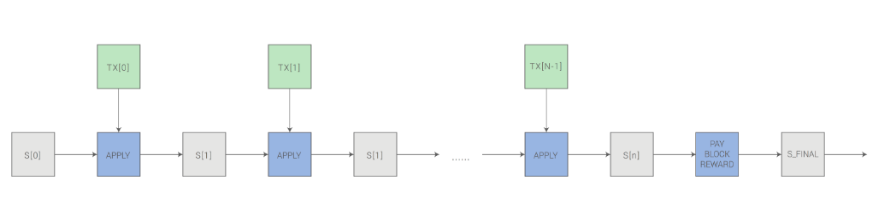
\includegraphics[width=0.8\textwidth]{Figures/Screenshot_20220507_131504.png}
    \caption{Diagrama que explica la mineria}
    \cite{web:block}
    \label{fg:block_diagram}
\end{figure}
La red de ethereum siempre se asegura que se genera un bloque cada 12 segundos.
Estos 12 segundos son una especie de latido que muestra la salud de la red de ethereum. Para mantener siempre ese ritmo, se ajusta la dificultad de minado. El proceso de minería sigue los siguientes pasos.
\begin{enumerate}
    \item Se genera una transacción y se firma con la clave privada.
    \item El usuario comparte la petición a toda la red de ethereum desde un minero.
    \item En algún momento de esos 12 segundos, un minero puede llegar a agregar cientos de transacciones en un posible bloque, en una manera que maximiza las comisiones de transacción. Todo esto mientras están por debajo del limite de gas.
    \begin{enumerate}
        \item Verifica la legitimidad de la transacción: Por ejemplo que la firma corresponde al mensaje y que la cuenta tenga liquidez.
        \item Inicia el proceso de \textit{proof of work}.\\ 
        Este proceso se basa en los siguientes parámetros. Dificultad del bloque ex:
        \texttt{3,324,092,183,262,715}, mixHash ex.\\ \texttt{0x44bca881b07a6a09f83b130798072441705d9a665c5ac8bdf2f39a3cdf3bee29} y la sal (número hexadecimal aleatorio) 
        \texttt{0xd3ee432b4fb3d26b}. \textit{Proof-of-work} es una carrera entre todos los mineros de la red para ver quien puede generar un \textit{hash} \cite{web:hash}. Cuando se genera un \textit{hash} con SHA 256 ex. \\
        \texttt{ba7816bf8f01cfea414140de5dae2223b00361a396177a9cb410ff61f20015ad} se busca que tenga que tenga una cierta cantidad de ceros al principio. La dificultad del bloque es cuántos \textit{hashes} pueden ser correctos para ese bloque. Cuanto menor sea el número, más difícil es verificar ese bloque.
    \end{enumerate}
    \item Eventualmente, algún minero conseguirá solucionar el puzzle criptográfico y nuestro mensaje estará aceptado en la \textit{blockchain}. Ese bloque contiene el \textit{checksum} (Suma de verificación \cite{web:checksum}) de todos los elementos internos.
    \item El resto de la red, al escuchar que un minero ha conseguido solucionar el bloque, lo verifica y si es correcto lo toma como el estado canónico de la red.
    \item Por ultimo los mineros borran de su memoria la lista de su \textit{mempool}. \cite{web:mining}
\end{enumerate}
\textbf{Limitaciones}\\
\textit{Proof-of-work}, como se ha explicado, es una operación computacionalmente intensa. En una red congestionada como está en estos momentos \cite{web:gas_price}, la dificultad de los bloques está explotada. Aún así, el consumo energético, comparando con otras \textit{blockchains} famosas, es inferior \ref{fg:consumo}. Esto hace que si tenemos aproximadamente 70 transacciones en un bloque, estamos gastando 5880000 Wh.
\begin{figure}[H]
    \centering
    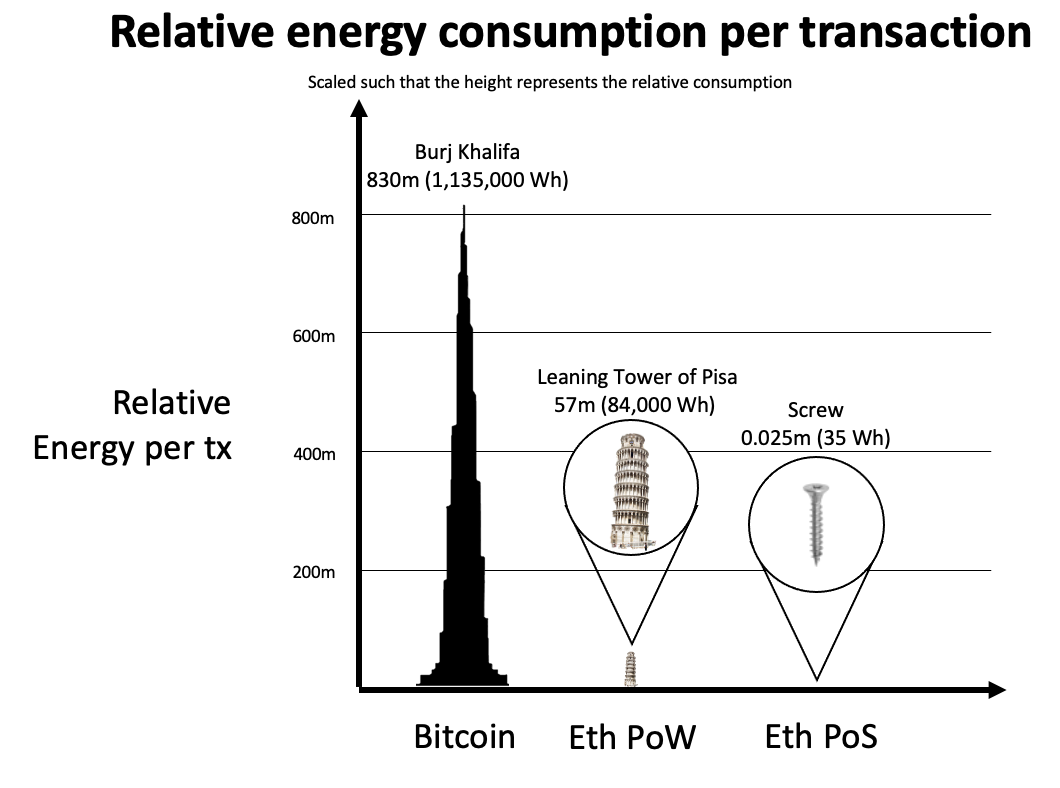
\includegraphics[width=0.6\textwidth]{Figures/consumo.png}
    \caption{Diagrama comparativo de consumo energético por transacción}
    \label{fg:consumo}
    \cite{web:eth_energy}
\end{figure}
Ethereum quiere actualizar su método de verificación a \textit{proof-of-stake}. Esto cambiaría a un modo de verificación computacionalmente caro a otro que no lo es tanto. Antes de que ese cambio ocurra, Ethereum seguirá consumiendo en un año lo mismo que Finlandia y tendrá una huella de carbono comparable a Bulgaria \cite{web:carbono}.
A fecha de publicación de este proyecto, Ethereum 2.0 no está implementado. Desde 2016 se lleva retrasando una bomba de dificultad para migrar a los usuarios, pero aún \textit{no ha explotado}. Esta bomba existe para evitar que se cree una copia. Esto hará que la dificultad crezca de manera exponencial hasta que minar un nuevo bloque sea imposible. Se lleva retrasando año tras año, hasta un total de 5 veces. Por ahora tiene fecha de junio de 2022. Aún así, en el EIP-4345 \cite{web:eip_bomb}, se da la posibilidad de retrasarlo aún más.
Hasta que no se haga el cambio de algoritmo de verificación, Ethereum seguirá contaminando. Esta implicación ética se investigará en el apartado correspondiente.
\subsection{Gas}
Como se ha explicado antes, se puede ejecutar código en la red de ethereum. Para proteger la red, existe una pequeña tarifa que hay que pagar por cada unidad de tiempo de ejecución. Así se evita la existencia de ataques por parte de actores malignos. Cuando una transacción se completa, se envía de vuelta el gas resultante al origen \ref{fg:message_diagram}.
\begin{figure}[h!]
    \centering
    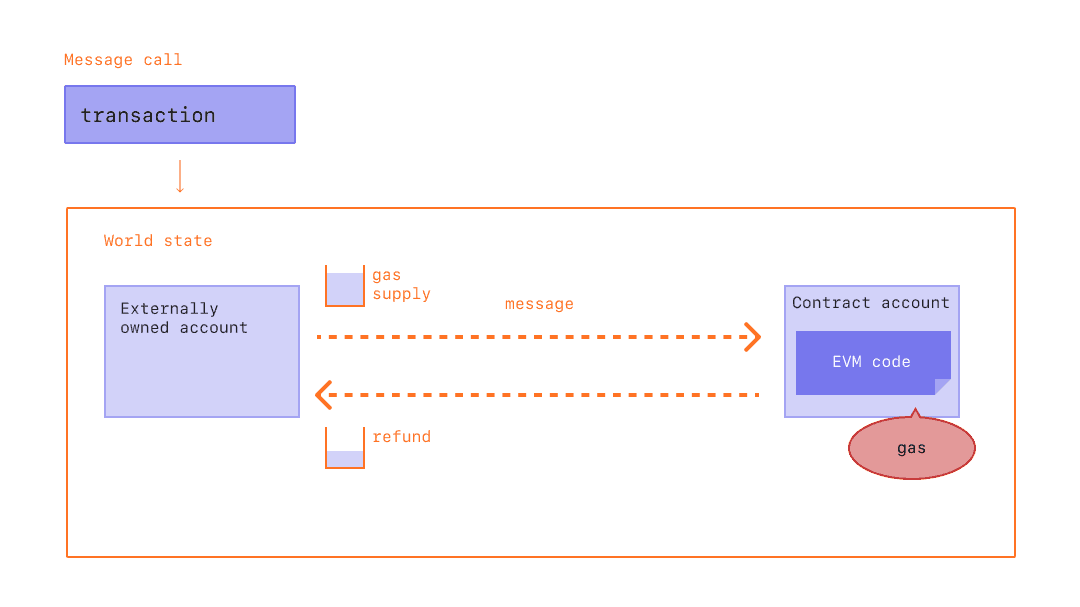
\includegraphics[width=0.8\textwidth]{Figures/gas-tx.png}
    \caption{Diagrama que explica el uso de gas}
    \label{fg:message_diagram}
\end{figure}
\begin{equation}
    max fee - (base fee + tip) = refund
\end{equation}
Después de la \textit{London update} \cite{web:london}, el gas en ethereum ha evolucionado para proteger más a los usuarios de posibles manipulaciones por parte de los mineros. Esta limitación se explicará más adelante.
\subsection{Smart Contracts}
Un \textit{smart contract} (Contrato inteligente \cite{web:scontract}) es un programa que vive en la \textit{blockchain}. A niveles prácticos, un contrato es como si fuese otra persona de la red con la que interactuamos.
Si nosotros tenemos la dirección
\begin{quote}
    \verb|0xc0ffee254729296a45a3885639AC7E10F9d54979|
\end{quote}
un contrato puede tener la dirección
\begin{quote}
    \verb|0x70E3Aed5aA1aac6EC39D114B7411DF6f1CC80671|
\end{quote}
Todos los mensajes compartidos entre los usuarios y un \textit{smart contract} quedan grabados para siempre en la cadena de bloques global. Como se ha dicho anteriormente, en Ethereum las transacciones se llaman mensajes, porque su contenido no es simplemente dinero, puede tener una infinidad de funciones.
\begin{lstlisting}
    pragma solidity 0.8.7;

    contract VendingMachine {
    
        // Declare state variables of the contract
        address public owner;
        mapping (address => uint) public cupcakeBalances;
    
        // When 'VendingMachine' contract is deployed:
        // 1. set the deploying address as the owner of the contract
        // 2. set the deployed smart contract's cupcake balance to 100
        constructor() {
            owner = msg.sender;
            cupcakeBalances[address(this)] = 100;
        }
    
        // Allow the owner to increase the smart contract's 
        // cupcake balance
        function refill(uint amount) public {
            require(msg.sender == owner, "Only the owner can refill.");
            cupcakeBalances[address(this)] += amount;
        }
    
        // Allow anyone to purchase cupcakes
        function purchase(uint amount) public payable {
            require(msg.value >= amount * 1 ether, 
            "You must pay at least 1 ETH per cupcake");
            require(cupcakeBalances[address(this)] >= amount,
            "Not enough cupcakes in stock to complete this purchase");
            cupcakeBalances[address(this)] -= amount;
            cupcakeBalances[msg.sender] += amount;
        }
    }
\end{lstlisting}
Tomando de ejemplo el código de la \textit{wiki} de Ethereum, se va a explicar su funcionamiento. \cite{web:sample_smart_contract}.
Solidity, el lenguaje de programación DSL (domain specific language \cite{web:DSL}) que utiliza la \textit{blockchain} Ethereum, tiene un paradigma de programación basado en objetos. Por eso mismo, su sintaxis es similar a los lenguajes \textit{C-like}, por ejemplo java.
En el siguiente bloque de código, especificamos la version de solidity que vamos a utilizar; En este caso y a fecha de publicación de este proyecto es la siguiente: \verb|0.8.7|.
\begin{lstlisting}
    pragma solidity 0.8.7;
\end{lstlisting}
Después podemos definir nuestro objeto. Para este ejemplo, vamos a crear una maquina de \textit{vending}.
\begin{lstlisting}
    contract VendingMachine {//...}
\end{lstlisting}
En este lugar, funcionaría de una manera parecida a un programa clásico en java. Las variables de ese objeto se pueden declarar directamente, estableciendo si son públicas o privadas. Ser pública significaría que esa variable es accesible por otros objetos, permitiendo utilizar su valor o modificarlo directamente. Ser privada, significa que solo puede ser usada por el objeto que la crea.
En nuestra máquina dispensadora, se va  a guardar la dirección del creador para poder por ejemplo reponer la maquina. Solidity tiene un tipo nativo que puede guardar direcciones directamente.
\begin{lstlisting}
    address public owner;
\end{lstlisting}
Ahora solo se necesita llenar la maquina. En este punto, podemos crear un mapa que asocie cantidades a direcciones concretas.
Si la dirección de nuestro contrato es \verb|0x70...0671| podemos hacer que si buscamos el valor asociado a esa dirección obtengamos el balance.
\begin{lstlisting}
    mapping (address => uint) public cupcakeBalances;
\end{lstlisting}
Para poder llenar la máquina nada más instalarla, existe el constructor. Un método constructor en java se ejecuta cuando se crea una nueva instancia del objeto con la \textit{keyword} \verb|new|. En este caso, nuestro constructor es llamado una vez se añade a la \textit{blockchain}. Por este motivo, nos cuesta gas hacer \textit{deploy} (despliegue) de un contrato.
\begin{lstlisting}
    // When 'VendingMachine' contract is deployed:
    // 1. set the deploying address as the owner of the contract
    // 2. set the deployed smart contract's cupcake balance to 100
    constructor() {
        owner = msg.sender;
        cupcakeBalances[address(this)] = 100;
    }
\end{lstlisting}
Por último, tenemos las funciones clásicas. En una maquina solo se puede añadir elementos y que alguien los compre. Estas funciones se pueden crear con la \textit{keyword} \verb|function|. Pueden comportarse como \textit{voids} o como una persona a la que pagar con \verb|payable|.
Gracias a \verb|require|, podemos crear puntos de control, que por ejemplo permitan que solo el creador pueda añadir más magdalenas a la máquina. No solo eso, sino que podemos asegurarnos que tengan el dinero necesario y que queden magdalenas en la máquina.
\begin{lstlisting}
    // Allow the owner to increase the smart contract's cupcake balance
    function refill(uint amount) public {
        require(msg.sender == owner, "Only the owner can refill.");
        cupcakeBalances[address(this)] += amount;
    }

    // Allow anyone to purchase cupcakes
    function purchase(uint amount) public payable {
        require(msg.value >= amount * 1 ether, 
        "You must pay at least 1 ETH per cupcake");
        require(cupcakeBalances[address(this)] >= amount, 
        "Not enough cupcakes in stock to complete this purchase");
        cupcakeBalances[address(this)] -= amount;
        cupcakeBalances[msg.sender] += amount;
    }
\end{lstlisting}
\textbf{Limitaciones}\\
La gran limitación de los \textit{smart contracts} es la inmutabilidad de la red. Una vez se publica ese contrato, no se puede actualizar. Si se descubre un fallo o se quiere cambiar la lógica se necesita volver a publicar el contrato. Esto implica que no solo el contrato sigue existiendo para siempre, sino que hay que direccionar a nuestros usuarios al nuevo contrato.
Como se explicará mas adelante, esto supone que hay que cambiar la dirección que le aportamos a los usuarios a través de nuestro \textit{payload} de js.
\subsection{Puntos débiles de la solución elegida}
Antes de la \textit{London Update} \cite{web:london}, los mineros podían llegar a manipular el precio ralentizando la ejecución y usando todo el gas del usuario. Esto suponía que los usuarios que quisieran hacer una transacción, se encontraban con la necesidad de llenar con más gas su transacción para que algún minero la ejecutase en un tiempo aceptable. El resto de usuarios, si querían que su transacción no tardase 30 minutos como mínimo, tendría que inevitablemente pagar más.
Para evitar eso, se introdujo un límite de gas en cada bloque. Ademas, los usuarios podían poner un rango de gas que estarían dispuestos a pagar. De esta forma, se busca que los bloques sean lo mas eficientes posibles.
Actualmente, tanto la dificultad de los bloques como el gas medio de transacción está disparado\cite{web:gas_price}. Esto hace que cualquier transacción tenga un coste añadido. Moderadores de r/ethereum dicen lo siguiente cuando son preguntados sobre si el alto precio del gas ``\textit{matará} '' a Ethereum:
\begin{displayquote}
    \textbf{High gas fees will kill Ethereum}\\
    This is one of those bizarre comments that pervades through crypto retail doesn't seem to make any sense. Overwhelming demand for a product will somehow... kill a project? It's like saying AMD and Nvidia are going to die soon because graphics cards are now grotesquely overpriced.
    No, the reality, like I said above, is that there's overwhelming demand for EVM blockspace and a limited supply of gas. Currently, the high fees shows there's incredible demand for Ethereum L1 blockspace, and people are willing to pay a steep premium for it.
    This is what gives the Ethereum network and ETH value. And in two months' time, there'll be a mechanism with EIP-1559 to accrue this value to every ETH stakeholder.
    Over time, we will see gas fees drop with a greater supply of gas - the reality is that there'll never quite be enough blockspace supply to satisfy global demand for EVM blockspace long term. There'll be rollups, there'll be hybrid solutions like zkPorter/Validium, there'll be sidechains/alternate chains, and there'll be centralized solutions. The ecosystem will work together to offer different trade-offs with decentralization versus transaction fees.
    \cite{web:reddit_ethereum}
\end{displayquote}
Aunque queda mucha discusión en los comentarios.
\begin{displayquote}
    Your answer for fees is far from being satisfying. Yes high fees will kill Eth. Your Nvidia example isn't the same thing.
    You know there are other successful blockchains coming strong. Avalanche for one has lots of Dapps on it. People will quit using Eth at some point if this doesn't change. Because other chains have already solved that problem...
    And I wouldn't care about any supply problem for a global demand, because this won't be an issue. We all use Eth because we have to and we all know it.
    \cite{web:reddit_ethereum_comment}
\end{displayquote}
Es un problema que los contribuidores de Ethereum tendrán que combatir y probar en una de la redes más grandes del mundo. Como Ethereum es código abierto, se pueden crear \textit{Ethereum Improvement Proposals} - EIP \cite{web:EIP}. De esta manera la comunidad puede mejorar y actualizar la red.
\section{Introducción a envíos de datos a través de un medio distribuido}
\begin{displayquote}
    IPFS is a distributed system for storing and accessing files, websites, applications, and data. \cite{web:ipfs_whatis}
\end{displayquote}
IPFS \cite{web:ipfs} es una red descentralizada que permite compartir datos de manera muy sencilla. IPFS consigue tener una mayor distribución del ancho de banda.
Todos los nodos de la red pueden estar conectados entre si teniendo una interconexión eficiente. Los ficheros subidos a IPFS tienen un CID (Content IDentifier). Ese CID es un registro permanente de la existencia de ese fichero como existe en el tiempo.
Cuando otro usuario busca tu CID \ref{fg:looking_for_CID}, pregunta al resto de los usuarios dónde esta el fichero. Cuando lo reciben, lo \textit{cachean} y se convierten en proveedores de tu fichero.
\begin{figure}[H]
    \centering
    
\includegraphics[width=0.2\textwidth]{Figures/svgviewer-png-output.png}
    \caption{Diagrama que explica la búsqueda de un CID}
    \label{fg:looking_for_CID}
    \cite{web:ipfs}
\end{figure}
Un usuario, puede anclar (pin) un fichero para guardar y proveerlo para siempre. En cambio, los contenidos que no tengan ese \textit{pin} serán descartados para liberar memoria. Los usuarios solo guardan lo que les interesa, más un pequeño índice para saber lo que tienen otros usuarios.
Todos los ficheros van acompañados de un \textit{checksum}; Si alguien intenta cambiar el fichero o sus datos, provocará un cambio en el \textit{hash}. Esto implica que se le asignará un CID distinto. Nuestros ficheros una vez subidos están seguros y serán resistentes ante la censura y la manipulación \ref{fg:keeping_IPFS_safe}.
En la siguiente sucesión de figuras, ponemos a prueba los pasos para iniciar una conexión.
\begin{center}
\begin{figure}[h!]
    \centering
    
\includegraphics[width=0.2\textwidth]{Figures/svgviewer-png-output(2).png}
    \caption{Diagrama que explica la protección ante censura}
    \label{fg:keeping_IPFS_safe}
    \cite{web:ipfs}
\end{figure}
\end{center}
\subsection{Servidores Star}
Para que los nodos se puedan encontrar, primero necesitan contactar con algún nodo conocido.
Para que eso ocurra, se tienen las siguientes opciones.
\begin{enumerate}
    \item Tablas de \textit{hashing} distribuidas.
    \item Paquetes \textit{broadcast} en la red local.
    \item Compartir listas de \textit{peers} con \textit{peers} conocidos.
    \item \textit{Trackers} o puntos de encuentro centralizados.
    \item Lista de servidores Star
\end{enumerate}
Los servidores son muy útiles ya que te devuelven información de dónde están tus \textit{peers} más cercanos con los que poder empezar a compartir.
Para comprender mejor la situación, vamos a ver unas figuras.
\begin{itemize}
    \item Tenemos un servidor Star que tiene metadatos de los \textit{peers} que están cerca.
    \item Las líneas grises son conexiones pasadas que han dejado el rastro del \textit{handshake} (saludo).
    \item Las líneas negras son conexiones activas de IPFS (libp2p).
    \item La figura verde quiere entrar a la red.
\end{itemize}
\begin{figure}[h!]
    \centering
    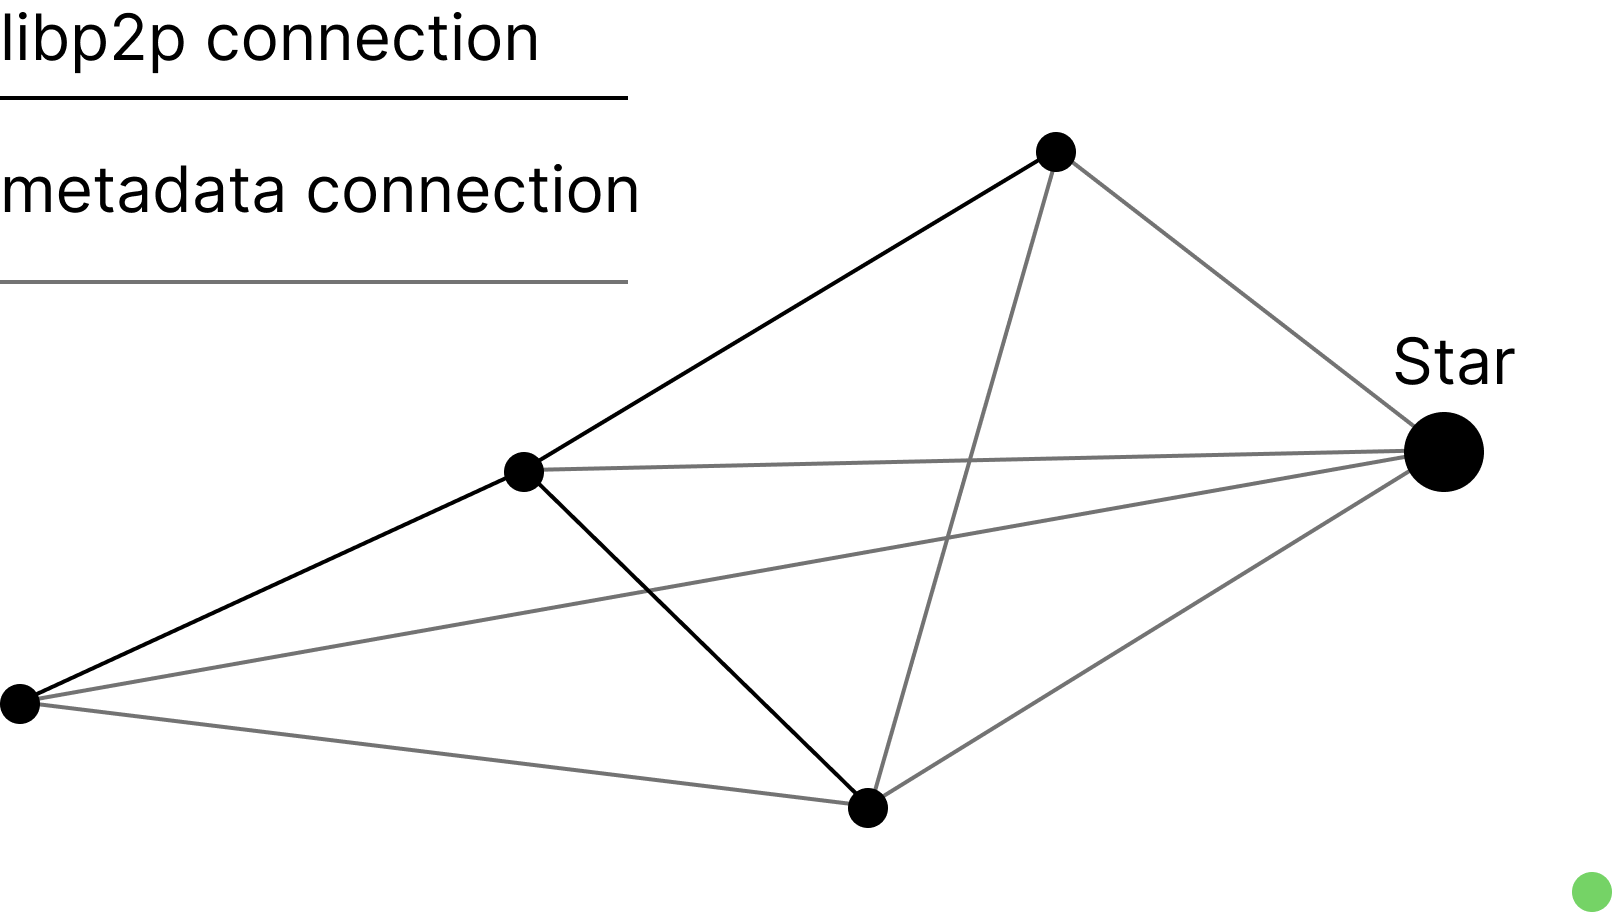
\includegraphics[width=0.7\textwidth]{Figures/Green wants to join(2).png}
    \caption{Diagrama en el que el nodo verde quiere entrar en la red IPFS}
    \label{fg:scanning_ipfs}
\end{figure}
\begin{figure}[h!]
    \centering
    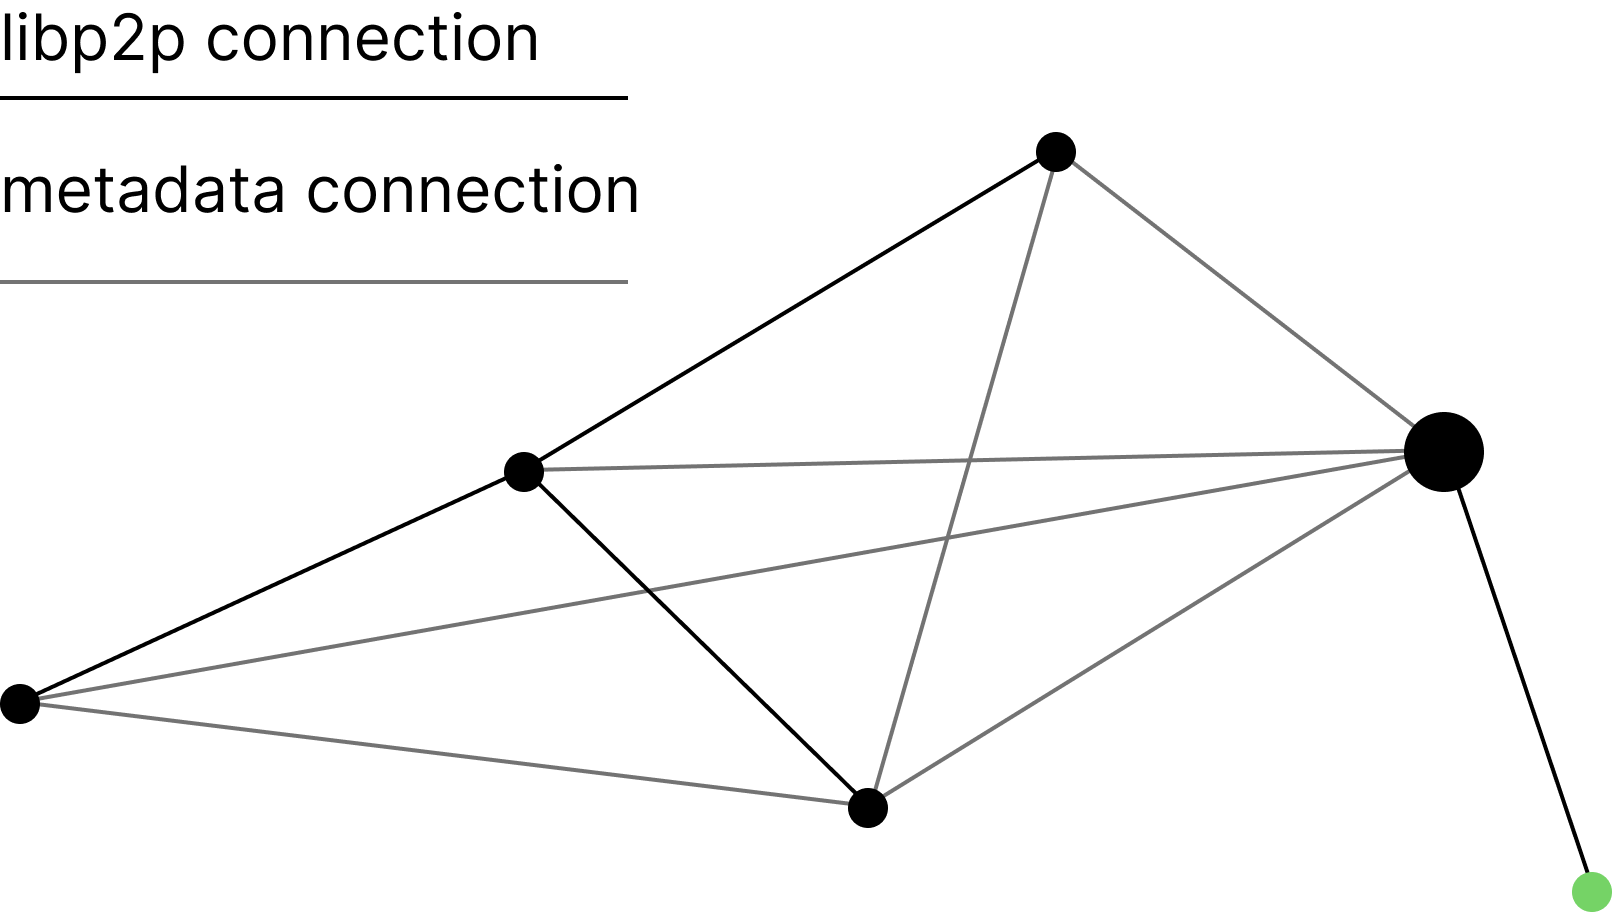
\includegraphics[width=0.7\textwidth]{Figures/Green ask Star for instructions.png}
    \caption{Diagrama en el que el nodo verde pregunta a Star dónde están el resto de las personas}
    \label{fg:asking_star}
\end{figure}
\begin{figure}[h!]
    \centering
    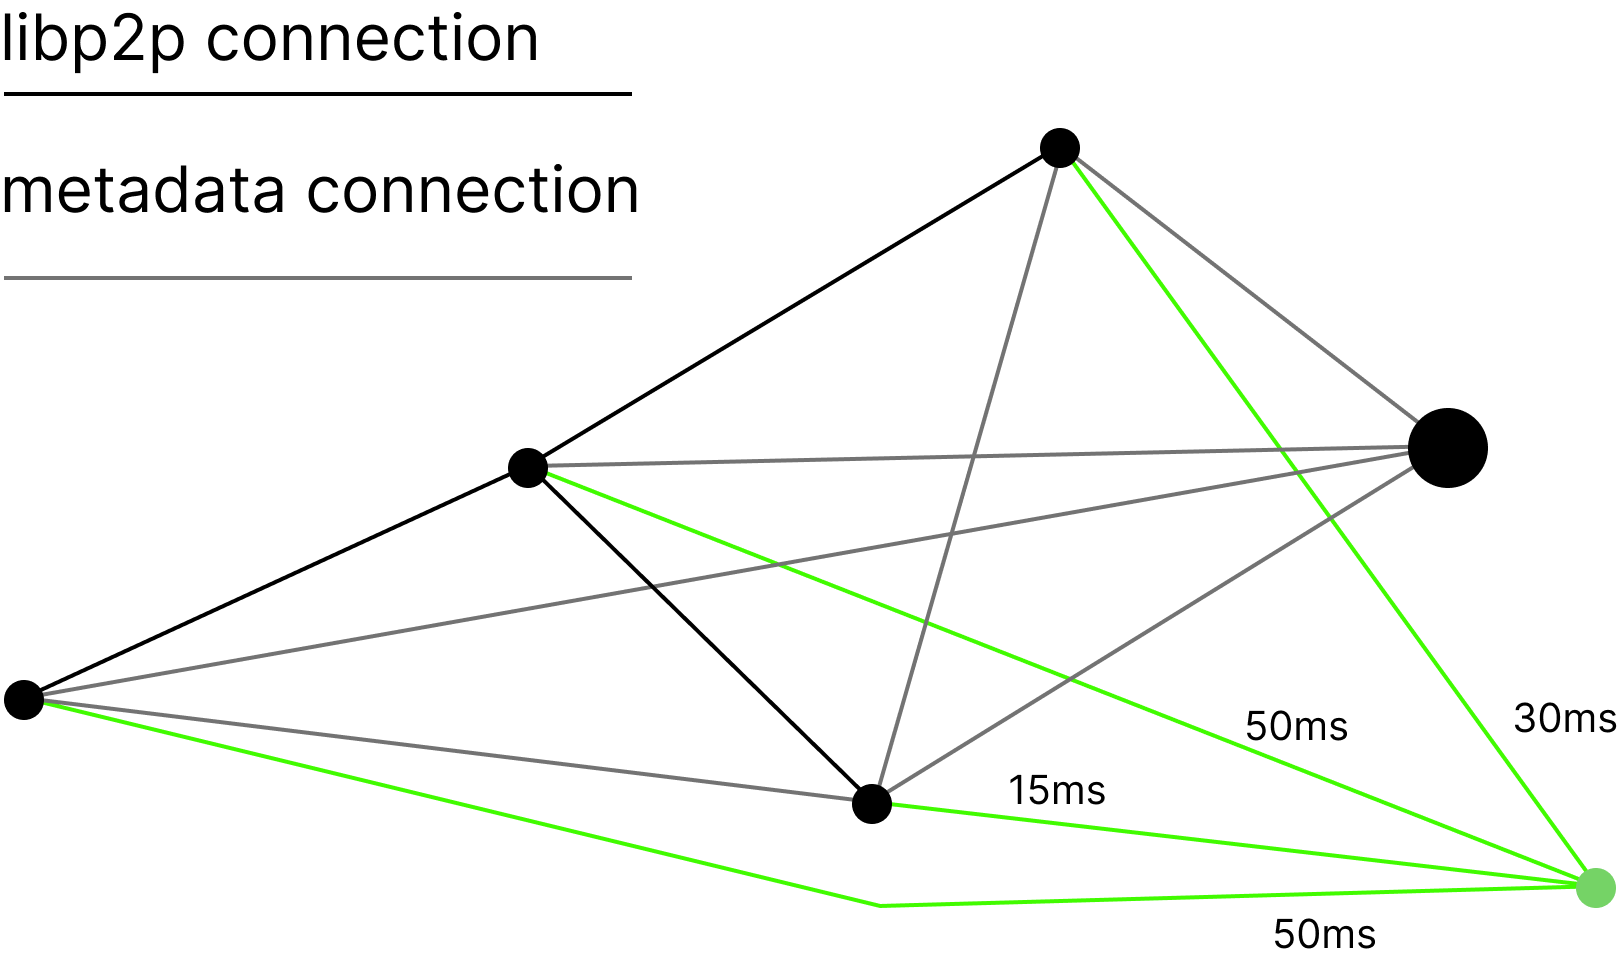
\includegraphics[width=0.7\textwidth]{Figures/Green scans the other peers.png}
    \caption{Diagrama en el que el nodo verde escanea sus alrededores para ver qué conexión es más eficiente}
    \label{fg:scanning_area}
\end{figure}
\begin{figure}[h!]
    \centering
    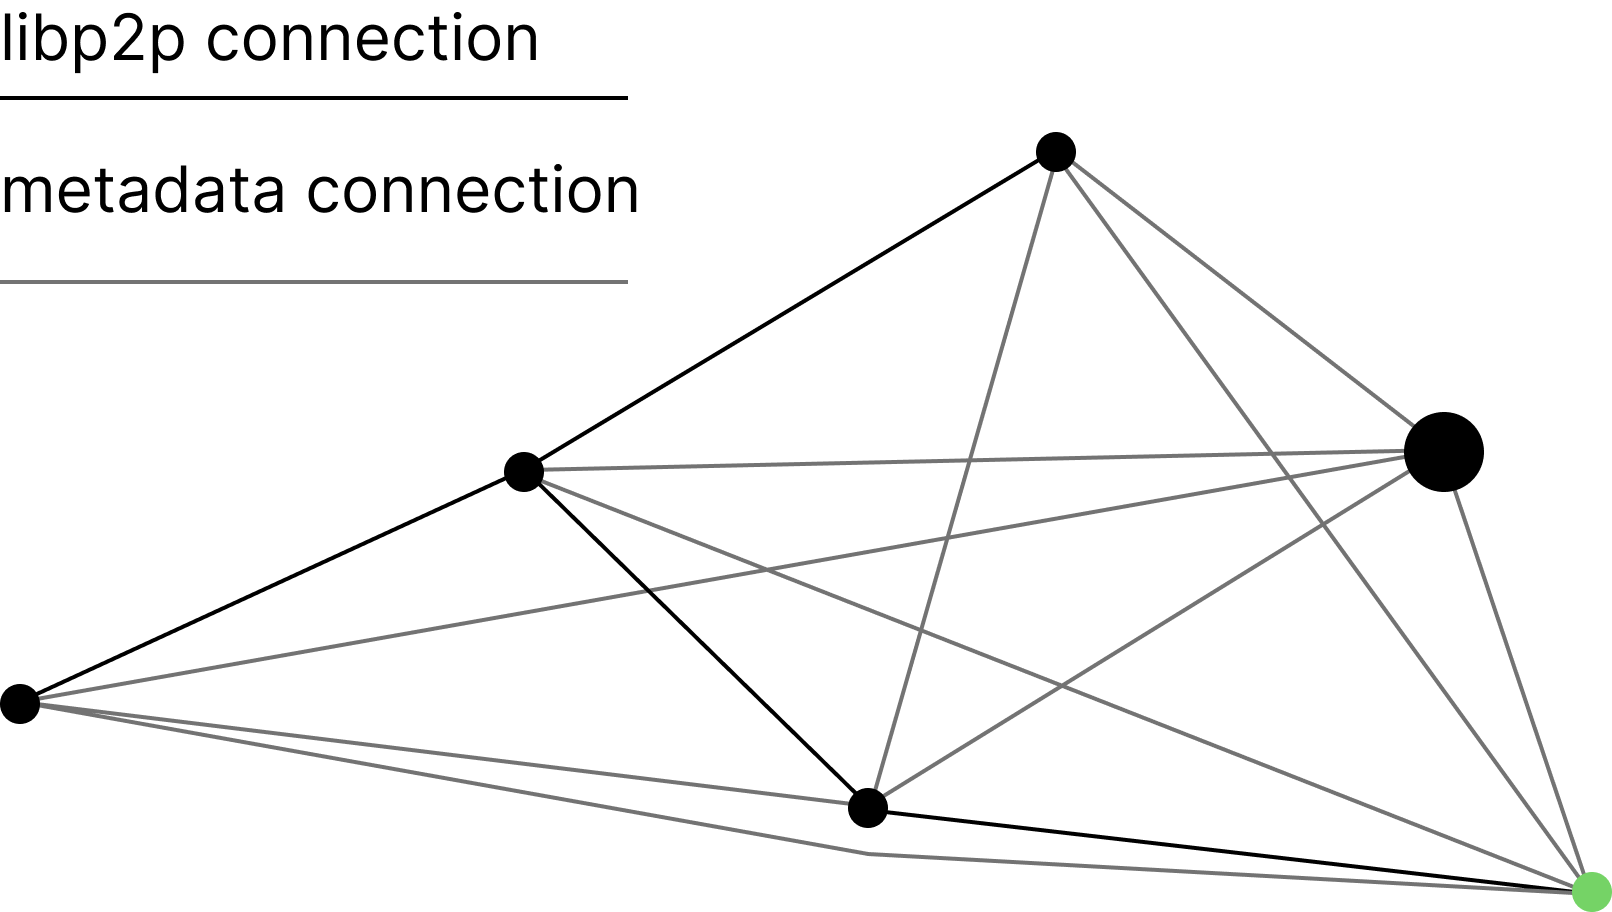
\includegraphics[width=0.7\textwidth]{Figures/Green finally joins(1).png}
    \caption{Diagrama en el que el nodo verde finalmente se conecta}
    \label{fg:connecting}
\end{figure}
\subsection{Nodos y relés}
Los nodos son los usuarios a los que se hacía referencia anteriormente. Estos nodos pueden ser: usuarios verídicos ejecutando \verb|js-ipfs| \cite{web:js-ipfs} en su navegador, o una instancia de \verb|go-ipfs| \cite{web:go-ipfs} o \verb|js-ipfs| en un servidor para garantizar nodos de alta velocidad.
Estos nodos tienen un repositorio en el que guardan fragmentos de datos que están alojando o bien que han pasado por él y ha cacheado.
Otra función principal de un nodo es retransmitir información. Para realizar esta función, tienen que estar conectados a otros nodos de la manera que hemos visto en el punto anterior.
\begin{figure}[H]
    \centering
    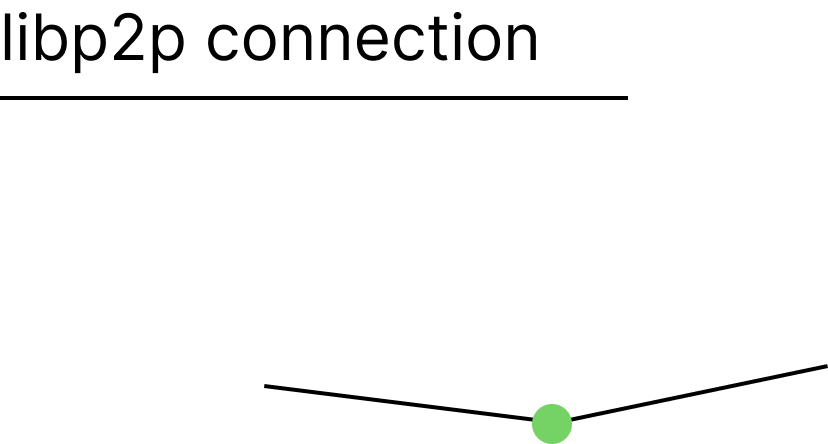
\includegraphics[width=0.4\textwidth]{Figures/Angulo 2.png}
    \caption{El nodo de color verde tiene un nivel de red 2. Ya que hay dos conexiones activas.}
    \label{fg:network_dgr}
\end{figure}
Primero vamos a ver el concepto de nivel de red. Las opciones predeterminadas de libp2p para el nivel ideal es \verb|6|. Un nivel entre \verb|4| - \verb|12| es un nivel \textit{aceptable}.
\begin{quote}
    Por simplicidad en los diagramas el \textit{Lower bound} (nivel inferior) = 2 y el \textit{Upper bound} (nivel superior) = 4.
\end{quote}
Viendo esto, necesitamos un modo inteligente en el que asegurar que todos los nodos reciben la información sin duplicidades.
\begin{figure}[h!]
        \centering
        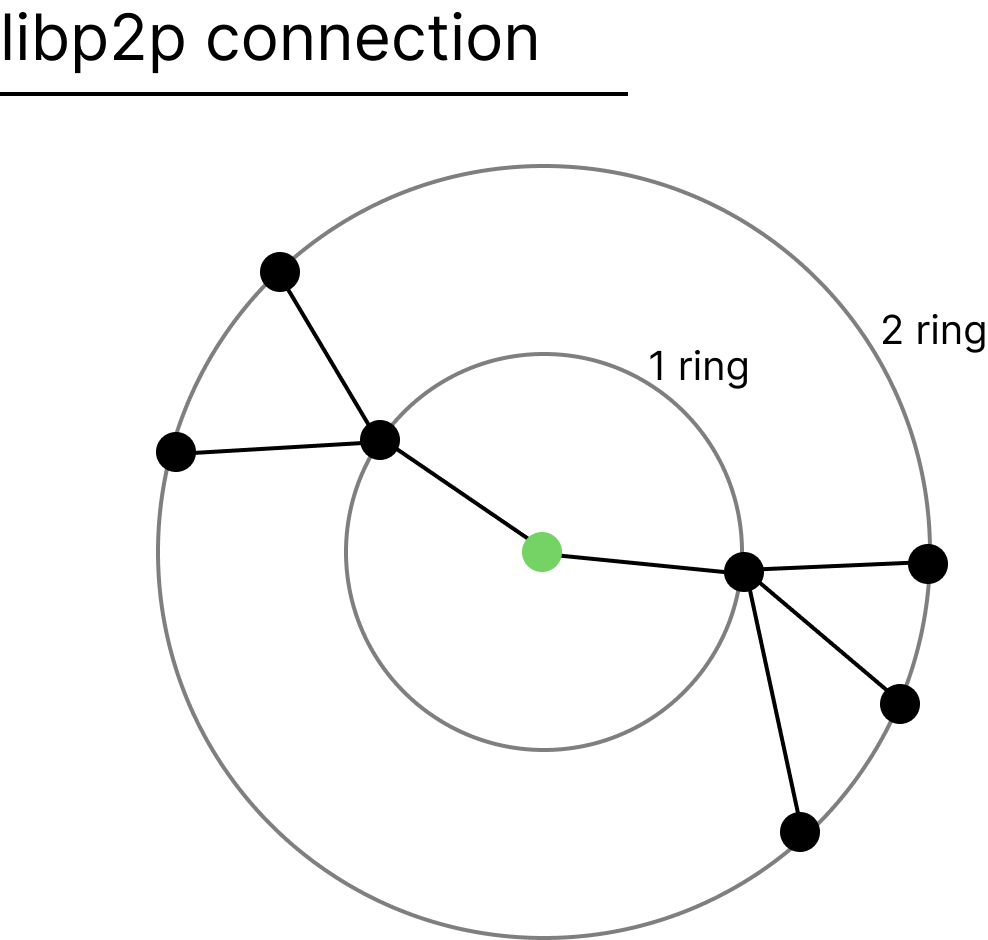
\includegraphics[width=0.5\textwidth]{Figures/Radios de comunicacion.png}
        \caption{Mapa de conexiones desde el punto de vista del nodo verde. \textbf{La conexión de metadatos ha sido omitida por razones de claridad.}}
        \label{fg:Mapa_de_conexiones}
\end{figure}
En la figura \ref{fg:Mapa_de_conexiones}, si un dato del ring 2 quiere llegar hasta el nodo verde, aparentemente, al no tener una conexión directa no podría hacerlo, pero como los nodos actúan de \textit{relays}, los datos pueden pasar por el ring 1 hasta llegar al nodo verde.
Al hacerlo, los nodos que viven en el ring 1, si los datos han pasado por ellos, pueden guardar esos datos para que si el nodo verde los vuelve a solicitar, se le envíen con menor latencia.
Aplicando \textit{pruning} (poda), el grafo anterior quedaría de la siguiente manera \ref{fg:mapa_optimizado}.
\begin{figure}[H]
    \centering
    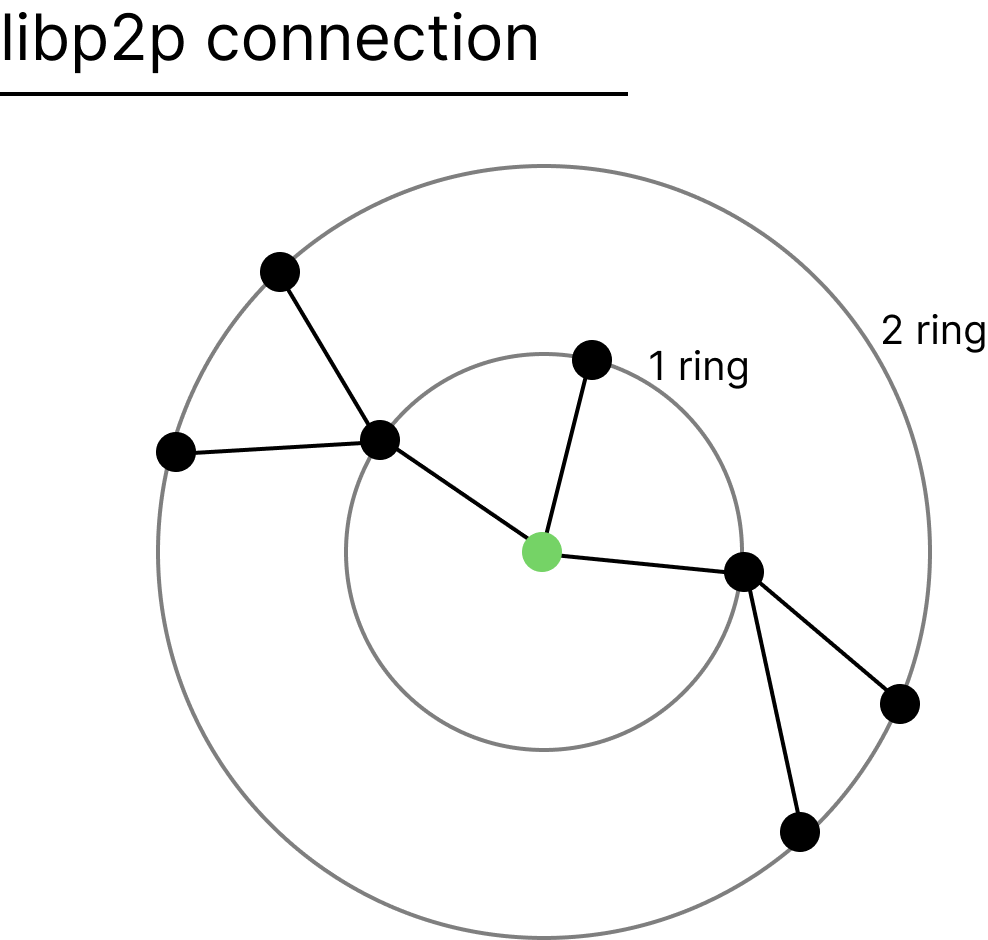
\includegraphics[width=0.5\textwidth]{Figures/Radios de comunicacion optimizado.png}
    \caption[El nodo verde optimiza la conexión]{El nodo verde optimiza la conexión. \textbf{El nodo movido, también calcularía cual seria su conexión óptima, pero todas las conexiones se ven desde el punto de vista del nodo verde.}}
    \label{fg:mapa_optimizado}
\end{figure}
Esto significa que como el nivel de conexión óptimo es 3, en la figura original \ref{fg:Mapa_de_conexiones} la red no es óptima. Nuestro nodo verde tiene 2 y el nodo en la parte inferior derecha tiene 4. Para poder generar un grafo más óptimo, el nodo verde tendría que tener 3 conexiones y el nodo en la parte inferior derecha también. Por eso mismo nuestro nodo verde inicia una nueva conexión óptima y el nodo en la parte inferior derecha borra una conexión, resultando en \ref{fg:mapa_optimizado}.
\subsection{PubSub}
PubSub \ref{fg:PubSub}, es una parte del \textit{spec} (especificación) de IPFS, fundamental para el funcionamiento del proyecto.
PubSub, permite subscribirse a un topic. Un \textit{topic} se define con un \verb|string|.
Pongamos como ejemplo que existen los siguientes topics.
\begin{figure}[h!]
    \centering
    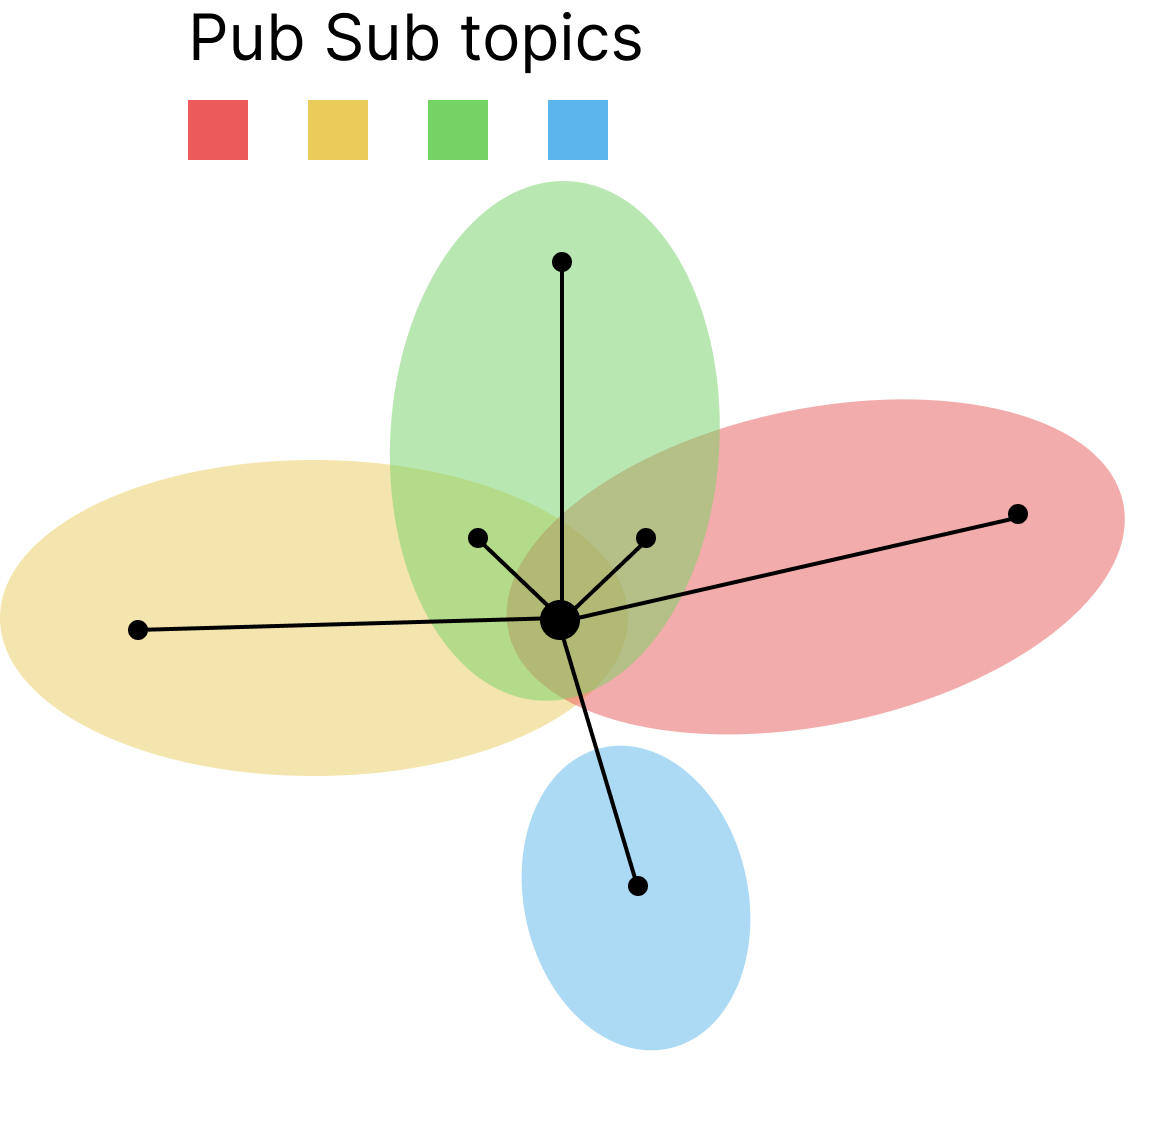
\includegraphics[width=0.7\textwidth]{Figures/Pub Sub.png}
    \caption{Diagrama explicando el funcionamiento de PubSub. Punto de vista del nodo central.}
    \label{fg:PubSub}
\end{figure}
\begin{itemize}
    \item \verb|Rojo|
    \item \verb|Verde|
    \item \verb|Amarillo|
    \item \verb|Azul|
\end{itemize}
El \textit{host} central, está subscrito a los \textit{topics} \verb|Amarillo|, \verb|Verde| y \verb|Rojo|.  Aun así, el nodo central está conectado a un nodo solo subscrito a un \textit{topic} \verb|Azul|. Esto se debe a que \verb|libp2p| intentará mantener una conexión saludable. Nuestro nodo no está solo interesado en escuchar a su \textit{topic}, sino ayudar a establecer una red saludable en la que hacer llegar la información necesaria a todos los nodos interesados.
\begin{figure}[H]
    \centering
    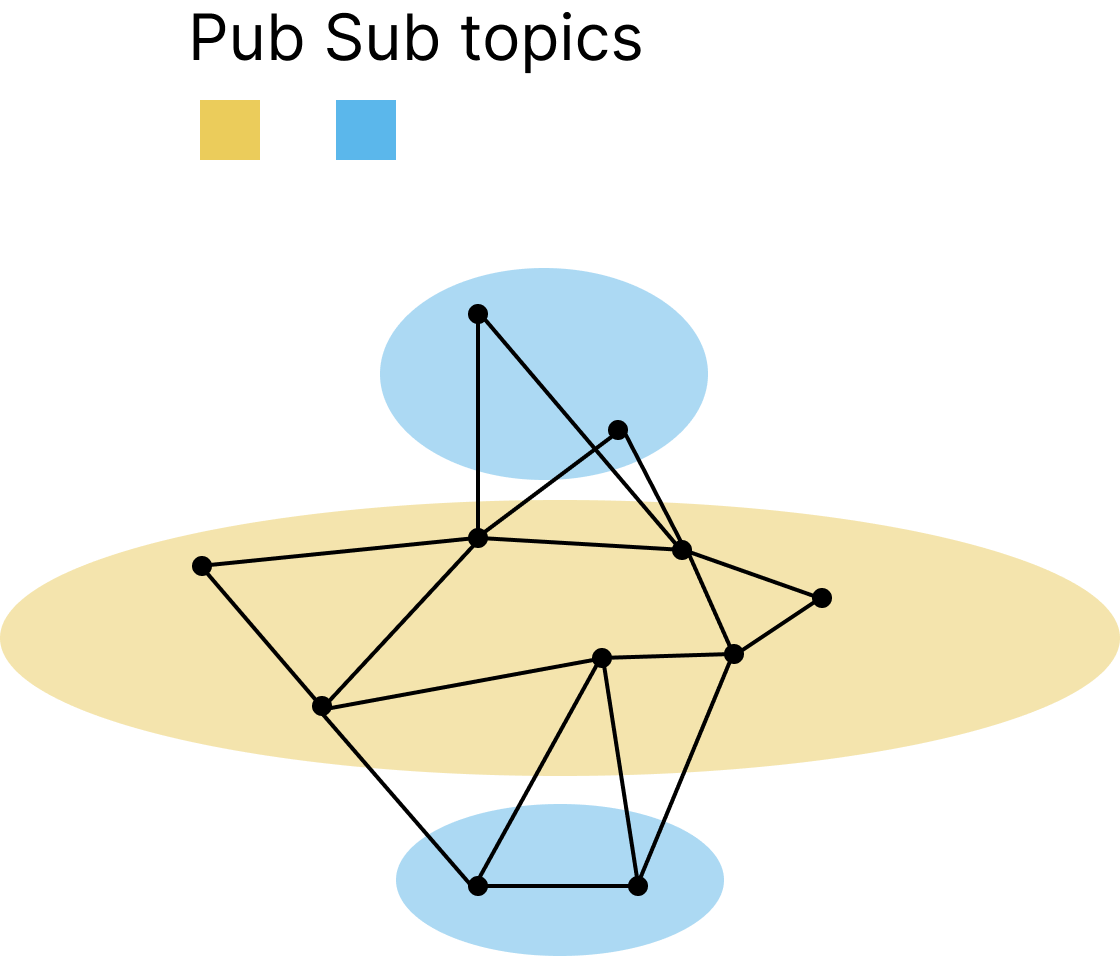
\includegraphics[width=0.7\textwidth]{Figures/Zonas multiples.png}
    \caption{Grafo de ejemplo para explicar la donación de temas.}
    \label{fg:zonas_multiples}
\end{figure}
En este posible grafo de conexión \ref{fg:zonas_multiples}, hay 4 hosts que están subscritos al tema \verb|Azul|. Si los \textit{host} que están escuchando al \textit{topic} \verb|Amarillo| no pasasen el mensaje, las dos zonas azules no estarían comunicadas.
Los nodos comparten todos los mensajes y guardan metadatos de los mensajes que pasar por ellos. Por eso, los nodos que escuchan al \textit{topic} amarillo, pueden hacer de relés y pasar todos los mensajes.
De este modo, IPFS nos permite crear una red global de envío de mensajes instantáneos de manera gratuita y con un sistema resistente a fallos, ya que nuestros paquetes tienen varias rutas por las que ir y reparten carga entre las rutas posibles.
\subsection{Alternativas}
A la hora de compartir información de manera distribuida, hay muchas opciones. Una de ellas, también muy popular en el presente, es webtorrent \cite{web:webtorrent}: Un librería que trae las tecnologías Torrent a la web.
Este proyecto, utiliza \verb|webrtc| lo mismo que IPFS para conseguir la funcionalidad. \verb|Webrtc| no se usa en el resto de la red. Significando que existe una brecha en la misma. Aunque los dos se basen en un archivo \verb|.torrent|, si no tienes \textit{peers} compartiendo esa información utilizando un cliente compatible, no puedes acceder a él.
\begin{figure}[H]
    \centering
    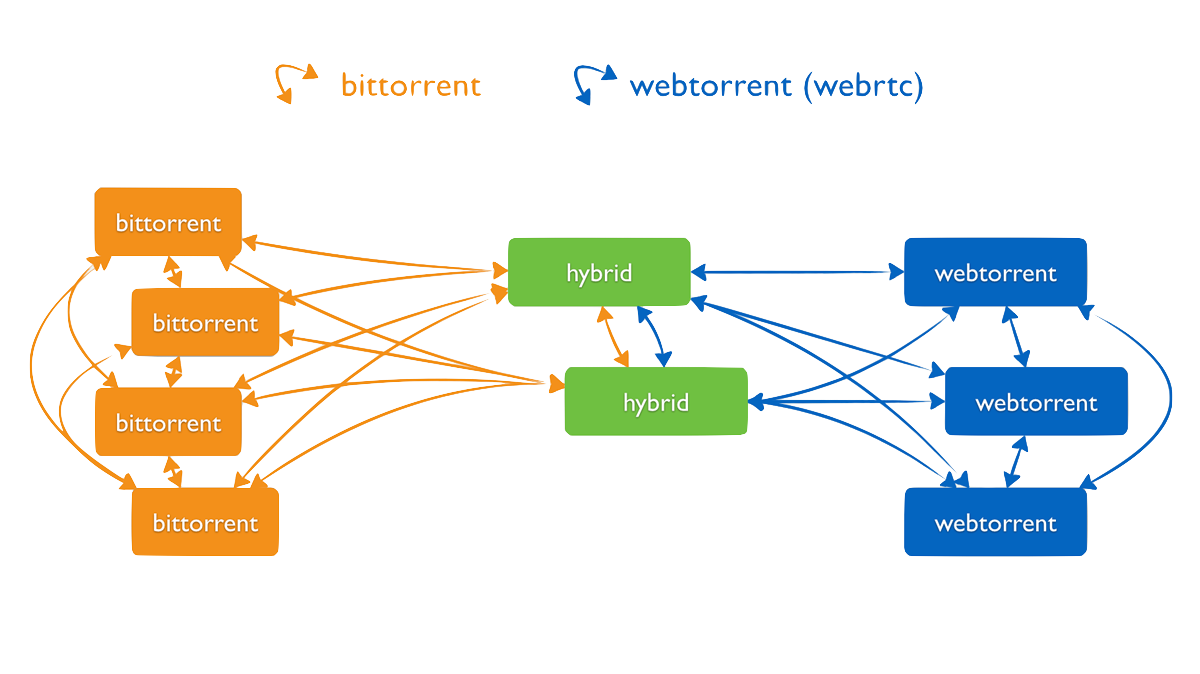
\includegraphics[width=0.6\textwidth]{Figures/68747470733a2f2f776562746f7272656e742e696f2f696d672f6e6574776f726b2e706e67.png}
    \caption{Diagrama explicando la división en la red de bit/web-torrent.}
    \cite{web:torrent}
    \label{fg:webtorrent}
\end{figure}
En la web, dan las herramientas a desarrolladores de programas \verb|torrent| a implementar un adaptador entre las dos redes. Por ahora solo \textbf{WebTorrent Desktop, Vuze, webtorrent-hybrid, Playback, instant.io y \(\beta\)Torrent} han implementado un adaptador, convirtiéndose en un nodo \textbf{\textit{hybrid}}.\\
% TODO: Explorar wormhole %
\textbf{Desventajas de utilizar WebTorrent}\\
Como ya se ha comentado hay una division en la red. Las tecnologías p2p se benefician de tener una gran cantidad de nodos. En cambio en este proyecto al haber una division, no se puede llegar a potencial teórico.
Otra gran desventaja es la \textbf{inmutabilidad}.
\begin{quote}
    \textbf{Is it possible to do live streaming with WebTorrent?}\\
    WebTorrent cannot do live streaming out-of-the-box, however you can build a live streaming solution on top of WebTorrent.
    Torrents are immutable. That means that once a torrent file is created, it cannot be changed without changing the info hash. So, how could one get around this limitation?
    A naive approach would be this: The content producer could take every 10 seconds of live content and create a torrent for it. Viewers would follow this \textit{feed} of torrent files (or info hashes) and download the content sequentially. Streamers would be around 10-20 seconds behind the live stream.
    This approach can definitely be improved, thougH Why not give that a shot yourself and share the code? \cite{web:webtorrent_faq}
\end{quote}
IPFS, aunque también sea inmutable por naturaleza para protegerse de censura y manipulación, implementa PubSub, una manera de poder propagar cambios en la red. 
Esto hace que en el archivo que reside en el DID solo exista el \textit{topic} y la identidad de esa persona. Como la base de datos es solo de esa persona, solo ella misma la que puede añadir identidades o retirarlas. Eso hace que las personas que estén escuchando al \textit{topic} de IPFS también puedan comprobarlo.
\newpage
\section{Introducción a la criptografía}
Este trabajo requiere criptografía para poder garantizar la seguridad de los datos compartidos. Como hemos visto, los datos compartidos en IPFS, por cualquier nodo que pasan, son cacheados para permitir una baja latencia en futuros accesos. Esto es un problema, ya que de manera predeterminada IPFS no incorpora encriptación de contenido.
\begin{quote}
    \textbf{IPFS docs}
    As a protocol for peer-to-peer data storage and delivery, IPFS is a public network: Nodes participating in the network store data affiliated with globally consistent content addresses (CIDs) and advertise that they have those CIDs available for other nodes to use through publicly viewable distributed hash tables (DHTs). This paradigm is one of IPFS's core strengths — at its most basic, it's essentially a globally distributed ``server'' of the network's total available data, referenceable both by the content itself (those CIDs) and by the participants (the nodes) who have or want the content.
    What this does mean, however, is that IPFS itself isn't explicitly protecting knowledge about CIDs and the nodes that provide or retrieve them. This isn't something unique to the distributed web; on both the d-web and the legacy web, traffic and other metadata can be monitored in ways that can infer a lot about a network and its users. Some key details on this are outlined below, but in short: While IPFS traffic between nodes is encrypted, the metadata those nodes publish to the DHT is public. Nodes announce a variety of information essential to the DHT's function — including their unique node identifiers (PeerIDs) and the CIDs of data that they're providing — and because of this, information about which nodes are retrieving and/or reproviding which CIDs is publicly available.
    So, why doesn't the IPFS protocol itself explicitly have a privacy layer built-in? This is in line with key principles of the protocol's highly modular design — after all, different uses of IPFS over its lifetime may call for different approaches to privacy. Explicitly implementing an approach to privacy within the IPFS core could "box in" future builders due to a lack of modularity, flexibility, and future-proofing. On the other hand, freeing those building on IPFS to use the best privacy approach for the situation at hand ensures IPFS is useful to as many as possible.\cite{web:ipfs_modularity}
\end{quote}
Hay dos tipos de encriptado:
\begin{itemize}
    \item Encriptado de transporte
    \item Encriptado de contenido
\end{itemize}
\subsection{Transporte}
La encriptación en el transporte \ref{fg:trasnporte} es usada cuando dos nodos quieren compartir información.
\begin{center}
    \begin{figure}[h!]
        \centering
        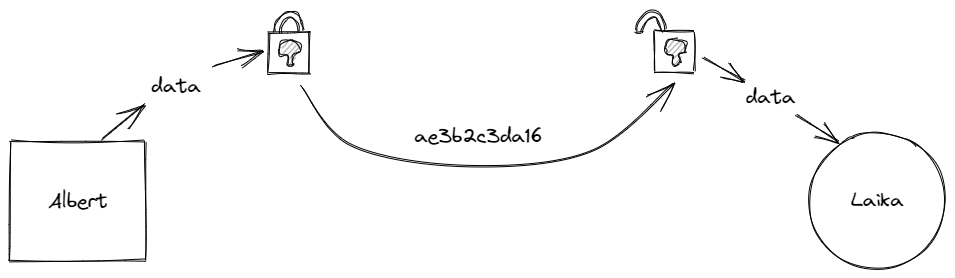
\includegraphics[width=0.7\textwidth]{Figures/transport-encryption.033b6a51.png}
        \caption{En esta figura, tenemos dos peers, que quieren enviar una información. IPFS encripta directamente la información haciendo imposible ver los datos \textbf{cuando están viajando de nodo en nodo}.}
        \label{fg:trasnporte}
        \cite{web:bias}
    \end{figure}
\end{center}
\subsection{Contenido}
La encriptación de contenido \ref{fg:contenido} se utiliza cuando se quiere asegurar que solo alguien que tiene la contraseña, pueda acceder al contenido.
\begin{center}
    \begin{figure}[h!]
        \centering
        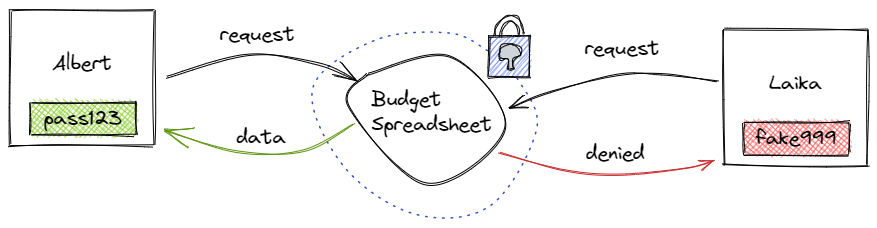
\includegraphics[width=0.7\textwidth]{Figures/content-encryption.adc5de58.png}
        \caption{En la figura, sin la contraseña correcta, Laika no puede acceder al fichero.}
        \label{fg:contenido}
        \cite{web:bias}
    \end{figure}
\end{center}
IPFS usa encriptación de transporte \ref{fg:trasnporte}, pero no encriptación de contenido \ref{fg:contenido}. Esto, según su \textit{wiki}, se hace para que no exista un \textit{bias} (sesgo de orientación \cite{web:bias}) a la hora de elegir qué tipo de encriptación es mejor para cada proyecto. Para este en concreto, se ha seleccionado una combinación de criptografía asimétrica con criptografía simétrica.
\subsection{XSalsa20 - Criptografía asimétrica}
La \textbf{criptografía asimétrica} (en inglés asymmetric key cryptography), \textbf{criptografía de clave pública} (en inglés public key cryptography) o \textbf{criptografía de dos claves} (en inglés two-key cryptography), es un sistema para poder compartir información utilizando claves públicas y privadas. Las claves públicas, como su nombre indica, son accesibles por todo el mundo. En cambio, la clave privada, tiene que permanecer protegida \cite{web:asimetrica}.
\begin{figure}[h!]
    \centering
    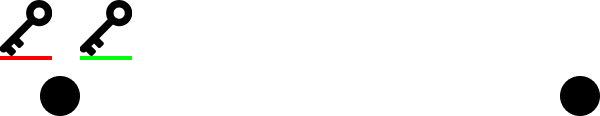
\includegraphics[width=0.7\textwidth]{Figures/Claves.png}
    \caption{Clave publica señalada en verde y la clave privada en rojo.}
    \label{fg:clave}
\end{figure}
Cuando el nodo de la derecha quiere enviar información a la que solo va a tener acceso el nodo de la izquierda, tiene que usar su clave pública \ref{fg:clave}.
\begin{figure}[h!]
    \centering
    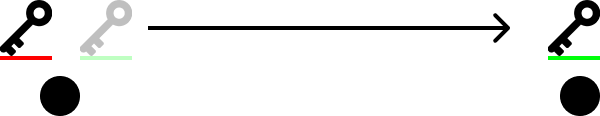
\includegraphics[width=0.7\textwidth]{Figures/Claves en movimiento(1).png}
    \caption{El host de la izquierda comparte su clave pública con el host de la derecha}
    \label{fg:movimiento}
\end{figure}
El nodo de la derecha, introducirá el mensaje en una caja y cerrará el candado utilizando esa llave. Ese candado solo puede ser abierto por la clave privada perteneciente al par original \ref{fg:movimiento}.
\begin{figure}[h!]
    \centering
    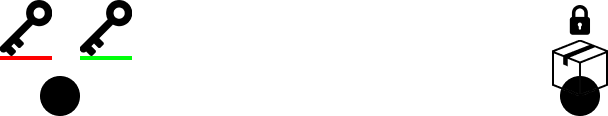
\includegraphics[width=0.7\textwidth]{Figures/Caja.png}
    \caption{El host de la derecha crea una \textit{caja}}
\end{figure}
Por último, lo único que queda es enviar esa caja a su destinatario; Esto se puede realizar por IPFS de manera segura.
NaCl pronunciada como ``sal'' es la librería de referencia, pero TweetNaCl \cite{web:tweetnacl}, consigue reducir el tamaño de NaCl, haciéndolo igual de rápido pero logrando que su código fuente quepa en 100 \textit{tweets}. De ahí su nombre.
\begin{quote}
    \textbf{Matthew D. Green, 2012}\\
    OpenSSL is the space shuttle of crypto libraries. It will get you to space, provided you have a team of people to push the ten thousand buttons required to do so. NaCl is more like an elevator—you just press a button and it takes you there. No frills or options.\\
    I like elevators. \cite{web:tweetnacl_elevator}
\end{quote}
\subsection{AES - Criptografía simétrica}
Aunque en teoría todas las comunicaciones se podrían hacer a través de criptografía asimétrica, para poder encriptar y desencriptar, se necesitan las claves de la cartera del usuario, estando limitados por el tamaño máximo que puedan soportar. Tenemos que comunicarnos con su cartera ya que nunca hay que dar la clave privada a nadie. Las claves privadas son propias y \textbf{siempre} deben serlo.
La criptografía simétrica se basa en una clave única. Cualquier entrada se puede encriptar y desencriptar con la misma clave. Para eso, a la hora de crear la caja para el usuario, generamos una contraseña aleatoria utilizando la \verb|api crypto| del navegador.
\begin{lstlisting}
    window.crypto.randomUUID()
\end{lstlisting}
\begin{quote}
    9fc2a1d0-5345-464c-a81e-a57a06b67669
\end{quote}
Después de esto se sigue el siguiente flujo.
\begin{itemize}
    \item Se encripta el fichero utilizando las \verb|apis| nativas de los navegadores.
    \item Anunciamos la existencia de un nuevo fichero en nuestro nodo de IPFS.
    \item En la caja introducimos el CID del fichero y la contraseña encriptada con la clave pública.
    \item Por último anunciamos por PubSub que se ha subido un fichero y que el destinatario puede abrirlo.
\end{itemize}
Para esta parte del proyecto se ha elegido AES ya que es muy popular, está soportado y tiene un buen historial de seguridad.
\newpage
\thispagestyle{empty}
\chapter{Objetivos y Alcance}\label{oya}
%Función que crea el título de capítulo y al cual se le da el nombre deseado a través de su parámetro obligatorio. Al no tener la función el “*” se escribirá también en el título del documento las palabras “Capítulo 1: …”. Además se indica, mediante la función “\label”, la correspondiente etiqueta que lleva asociada. La etiqueta sirve para que en caso de que luego se quiera hacer referencia al capítulo se haga llamando etiqueta tal que se escribiría “La información correspondiente a dicho tema se encuentra en el capítulo \ref{Int}.”

\thispagestyle{fancy}
%Función que determina que durante este capítulo se aplique el estilo Fancy.

\fancyhead[LE]{\thechapter.Objetivos y Alcance}


\section*{SSI}
SSI (Self sovereign identity) en ingles, es un un concepto en el la propia persona por existir, se representa a si mismo en internet. Esto, quiere decir que en internet nos dejaríamos de identificar utilizando correos electrónicos y pasaríamos a identificarnos por nuestra propia voluntad y una unión de clave publica y clave privada.

\section*{Introducción a las blockchain}
La blockchain, es un elemento importante para este proyecto. Su implementación, permite una comunicación segura y anónima entre personas, sin necesidad de ser verificada por terceros. Las blockchain, vienen en muchas formas y tipos, algunas siendo descentralizadas. Las mas populares, funcionan de manera puramente descentralizada, usando un sistema de prueba de trabajo para verificar todas las transacciones.

\newpage
\thispagestyle{empty}
\chapter{Metodología}\label{Metodología}
%Función que crea el título de capítulo y al cual se le da el nombre deseado a través de su parámetro obligatorio. Al no tener la función el “*” se escribirá también en el título del documento las palabras “Capítulo 1: …”. Además se indica, mediante la función “\label”, la correspondiente etiqueta que lleva asociada. La etiqueta sirve para que en caso de que luego se quiera hacer referencia al capítulo se haga llamando etiqueta tal que se escribiría “La información correspondiente a dicho tema se encuentra en el capítulo \ref{Int}.”

\thispagestyle{fancy}
%Función que determina que durante este capítulo se aplique el estilo Fancy.

\fancyhead[LE]{\thechapter.Metodología} 
%Función que se utiliza para indicar que en las páginas impares, aparezca en el encabezado en la parte izquierda, el número del capítulo con su correspondiente nombre.

\section{Desarrollo ágil}
Este proyecto nace de una idea tan amplia como el \textit{SSI}. No había requisitos iniciales y ni se conocía el alcance. Para poder estudiar las posibilidades tan amplias con las que se puede afrontar, se seleccionó la metodología SCRUM. Esta metodología está pensada para equipos con reuniones periódicas y \textit{sprints} de trabajo. Cada \textit{sprint} de trabajo tiene unos objetivos. Estos se comprobarán al final con una reunión.
En este caso, tras realizar un objetivo se aseguraba su funcionamiento y se comprobaban las metas. De este modo, se consigue enfocar los requisitos del proyecto al mismo tiempo que se asegura el funcionamiento global de la aplicación.
Como SCRUM es una metodología extensa y complicada, se va a introducir en este trabajo. Dicha metodología cuenta con cuatro pilares:
\begin{itemize}
    \item \textbf{Equipo SCRUM}\\
    Para poder realizar un trabajo, se necesita un motor para hacer mover las tareas.
    En el caso de este proyecto, el trabajo ha sido realizado por una sola persona. Las reuniones de control se realizaban con el director del proyecto al final de cada \textit{sprint}.
    \item \textbf{Backlog o lista de tareas}\\
    \begin{figure}[H]
        \centering
        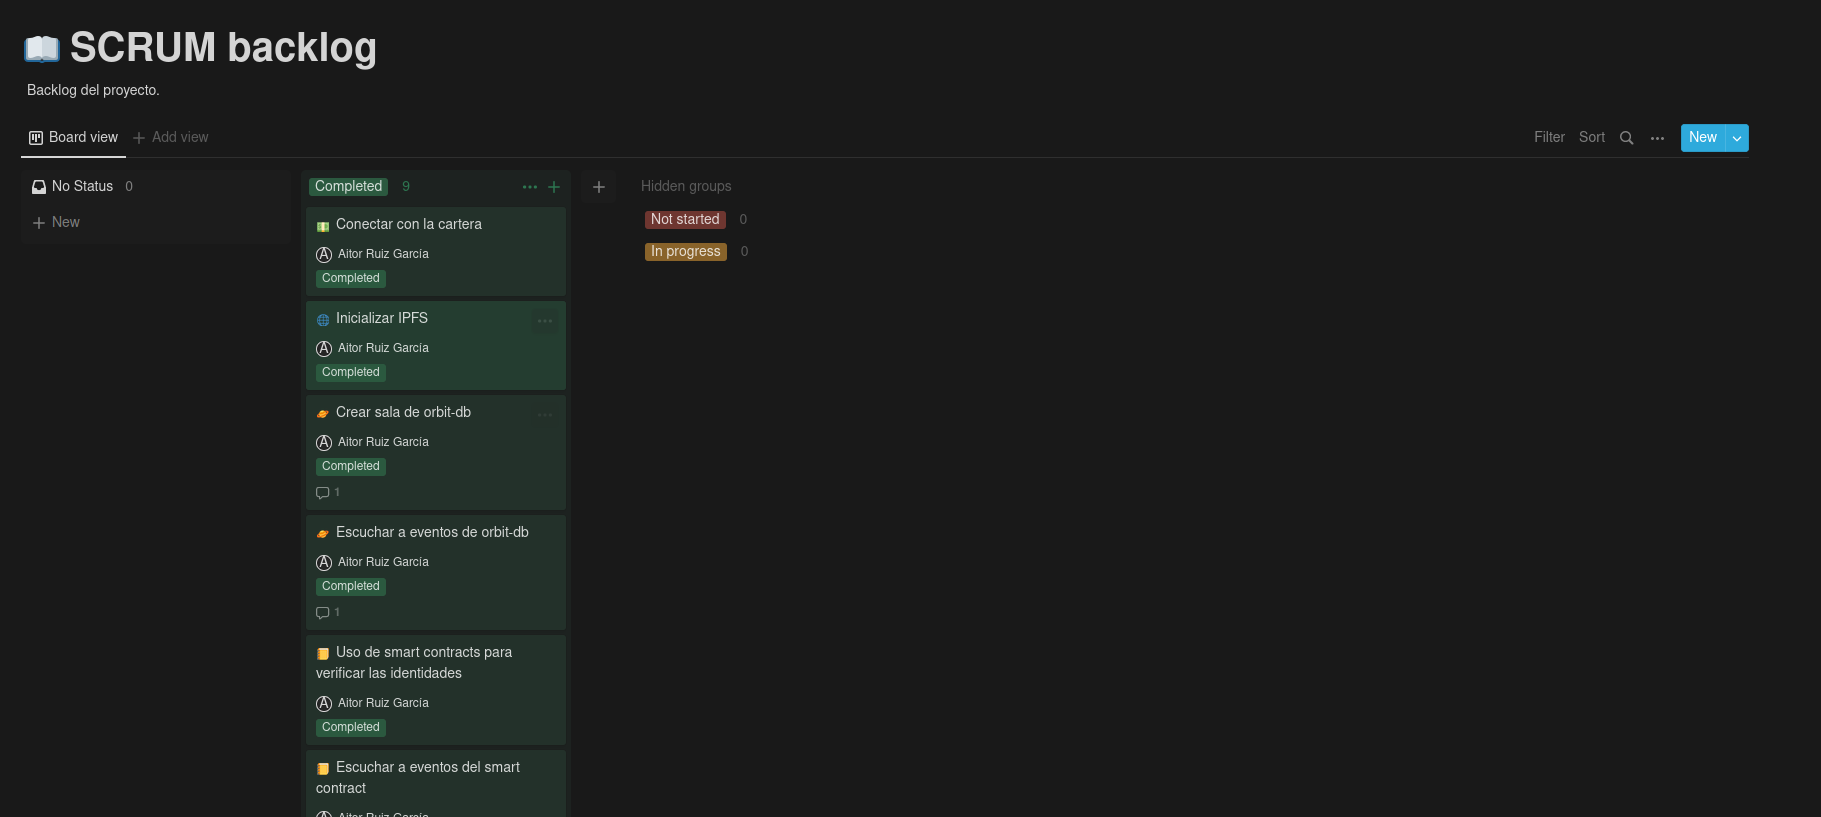
\includegraphics[width=0.8\textwidth]{Figures/Screenshot_20220601_182542.png}
        \caption{Imagen del backlog del proyecto}
        \label{fg:backlog}
    \end{figure}
    El desarrollo se ha estado controlando desde \verb|notion.so| \cite{web:notion}. Notion genera un archivo \verb|markdown|. Este fichero puede ser enriquecido con distintos \textit{widgets}. Uno de estos \textit{widgets} es una \textit{board view}. Esta inspirado en otras herramientas que permiten hacer \textit{backlogs} \ref{fg:backlog}.
    Se crearon temas que cumplían uno o varios requisitos del proyecto al mismo tiempo y que estaban relacionados entre sí. Estas tarjetas pueden ser desplazadas dependiendo del estado en el que se encuentran.
    \begin{itemize}
        \item \verb|No iniciado|
        \item \verb|En proceso|
        \item \verb|Completada|
    \end{itemize}
    Dentro de estas tarjetas se puede escribir y anotar elementos, por ejemplo: las horas invertidas en el desarrollo. Esto resulta útil para las reuniones y para el presupuesto.
    \item \textbf{\textit{Sprint}}\\
    Cuando se completa un \textit{sprint}, si se ha realizado la tarea correspondiente, la tarjeta deberá ser desplazada a \verb|completada|.
    En esta tarjeta, si se selecciona, se puede acceder a la información en su interior \ref{fg:tarjeta}.
    \begin{figure}[h!]
        \centering
        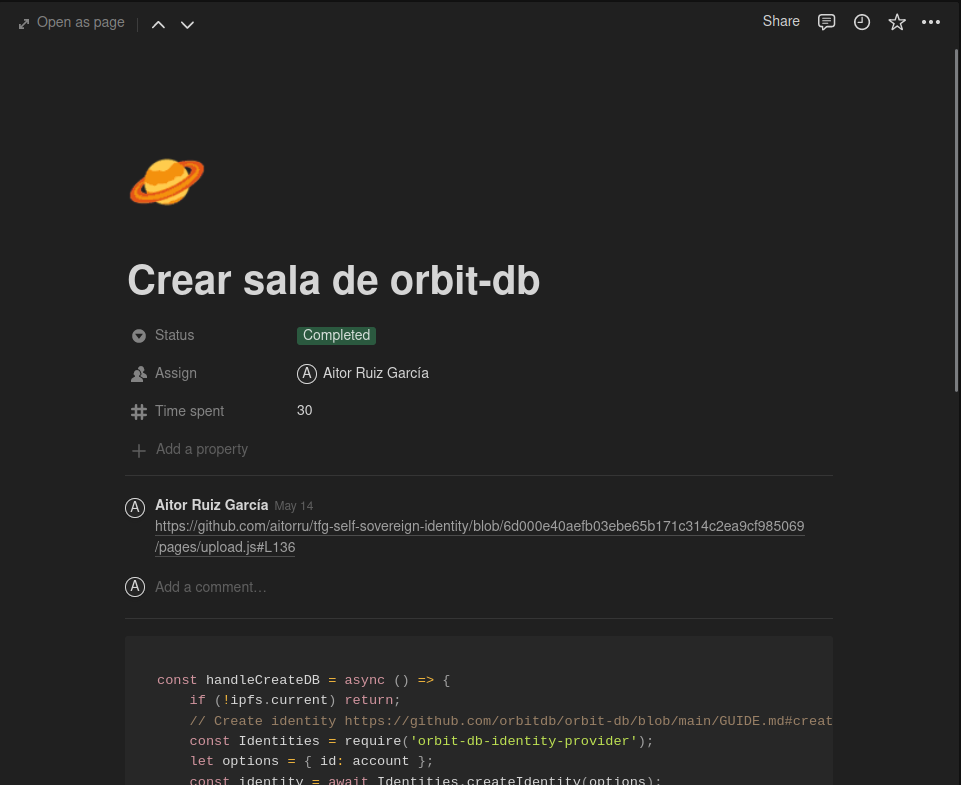
\includegraphics[width=0.7\textwidth]{Figures/Screenshot_20220601_181036.png}
        \caption{Imagen de los datos dentro de una tarjeta.}
        \label{fg:tarjeta}
    \end{figure}
    \item \textbf{Reuniones de seguimiento (bisemanales)}\\
    Para hacer las reuniones, se necesita disponer un guion donde se apuntará información útil asociados a la tarjeta. Ese conocimiento puede ser utilizado para el resto de los \textit{sprints}.
\end{itemize}
\section{Herramientas de desarrollo}
Un elemento fundamental para el desarrollo de esta aplicación ha sido \verb|Next.js| \cite{web:next.js}. Es un \textit{framework} \cite{web:framework} para generar paginas estáticas, con capacidad de utilizar SSR (renderizado de servidor \cite{web:ssr}) e ISR (renderizado estático incremental \cite{web:isr}).
En el apartado \textbf{Herramientas utilizadas}, se explicará por que se ha elegido un \textit{framework} basado en React. Aun así, solo estamos interesados en dos aspectos:
\subsection{Páginas estáticas}
Como hemos dicho anteriormente, en IPFS se pueden subir ficheros. Por lo cual podemos subir archivos \verb|.html|.
En el esquema de acceso clásico en una página, todos los usuarios acceden a un servidor centralizado \ref{fg:centralizado}.
\begin{figure}[H]
    \centering
    
\includegraphics[width=0.5\textwidth]{Figures/Centralizado.png}
    \caption{Imagen para explicar la centralización de un servidor. \textbf{El nodo con mayor tamaño es el servidor, el resto son usuarios que quieren conectarse.}}
    \label{fg:centralizado}
\end{figure}
Una implementación que cuente con más recursos, puede tener más nodos centralizados más cerca de sus usuarios, pero eso solo se lo pueden permitir organizaciones con muchos recursos.
Cuando una página no dispone de más servidores repartidos por el mundo, solo tiene un punto de acceso. IPFS viene al rescate ya que todos los ficheros que son compartidos, son \textit{cacheados}. Haciendo que cuanto más se use un fichero, más rápido se accederá a él.
Todos los ficheros estáticos pueden ser alojados en IPFS y visitados de la siguiente manera: tomando de ejemplo la documentación de IPFS \cite{web:ipfs_whatis}, imaginemos que queremos acceder a Wikipedia \cite{web:wikipedia_main}.
El servidor de Wikipedia puede estar al otro lado del mundo o en otro planeta. Aun así, en tu cercanía, es probable que otra persona también quiera acceder a Wikipedia. Para eso, se puede buscar si alguien tiene la página en la red de IPFS.
\begin{quote}
    \verb|/ipfs/QmXoypizjW3WknFiJnKLwHCnL72vedxjQkDDP1mXWo6uco/wiki|
\end{quote}
Si se introduce este DID en el navegador, no significa nada, ya que de manera nativa un navegador no puede convertirse en un nodo de IPFS. Por eso mismo, se necesita una manera de ejecutar \verb|js-ipfs| (una librería que se explicará más adelante) para poder recibir el fichero.
Existen muchas puertas de entrada \ref{fg:ipfs_entry} e incluso se pueden crear nuevas.
\begin{figure}[H]
    \centering
    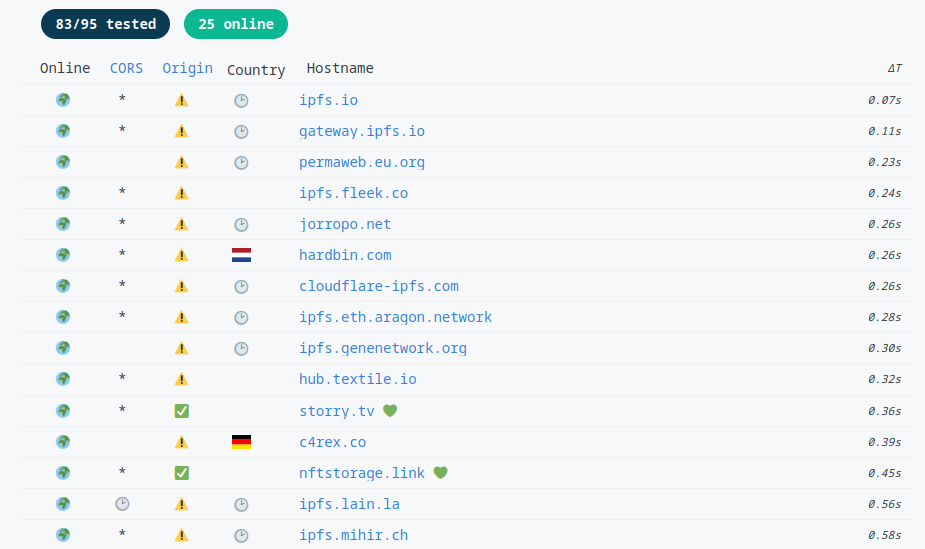
\includegraphics[width=0.7\textwidth]{Figures/ipfs_entry.png}
    \caption{Imagen de puntos de acceso de IPFS}
    \cite{web:gateways}
    \label{fg:ipfs_entry}
\end{figure}
Por simplicidad vamos a utilizar el \textit{gateway} de los creadores. \textbf{No significa que sea oficial}, eso no existe en el mundo distribuido.
\begin{quote}
    \url{https://ipfs.io/ipfs/QmXoypizjW3WknFiJnKLwHCnL72vedxjQkDDP1mXWo6uco/wiki/}
\end{quote}
De esta manera, tenemos acceso a una página de Wikipedia distribuida.
Esto también se puede aplicar al proyecto ya que Next.js de manera predeterminada, solo exporta ficheros estáticos. Esto resulta perfecto para IPFS.
\subsection{Separación de código y empaquetado}
Todas las librerías de web 3.0, están en un estado muy temprano y por ende no están optimizadas para ocupar poco espacio. Aunque nuestra página pueda estar alojada en IPFS y resulte en tiempos de respuestas más bajos, no significa que no haya que optimizar el tiempo de descarga del \textit{bundle} (paquete) de js. Para comprender mejor el problema y cómo poder aliviarlo, se va a poner un ejemplo. Next.js, aunque exporta HTML estático, es un framework que utiliza React para construir la interfaz. Más adelante, se explicará qué es React y por qué está seleccionado para este proyecto. Por ahora solo hay que saber que es un archivo de \verb|.js| que nuestro navegador tiene que ejecutar para que nuestra página pueda hacer algo útil.\\
En JavaScript, hay dos maneras de importar funcionalidad en un proyecto:\\
\textbf{Require}\\
\begin{lstlisting}
    // Este codigo no es recomendable.
    const react = require('react');
\end{lstlisting}
\noindent\rule{\textwidth}{0.4pt}
\textbf{Modules}\\
\begin{lstlisting}
    import react from 'react';
\end{lstlisting}
La diferencia principal es que require es síncrono e import es asíncrono.
Si es síncrono, cada instrucción se ejecuta una detrás de la anterior. En cambio con import, se deja cargando y se pasa a la siguiente instrucción.
Aunque los módulos están gradualmente adoptados \cite{web:canIuse} y han sido añadidos al \textit{spec} \cite{web:ecma}. A fecha de creación de este proyecto, \verb|Next.js| \cite{web:next.js} está configurado para hacer todo su código compatible con EC6, el \textit{spec} de 2015.
\begin{quote}
    Next.js supports \textbf{IE11 and all modern browsers} (Edge, Firefox, Chrome, Safari, Opera, et al) with no required configuration. \cite{web:next_supported}
\end{quote}
\begin{center}
    \begin{table}[h!]
        \begin{tabular}{p{0.3\linewidth}  p{0.6\linewidth}}
            \textbf{Modules} & \textbf{Require} \\ \hline
                \verb|import react from 'react';|
            & 
\verb|use strict';|

\verb|var _react = require('react');|
             \\
            Como vemos, nuestro import compacto y asíncrono en el spec de 2015, se convierte en un conjunto de código síncrono y extenso. & 
\verb|var _react2 = _interopRequireDefault(_react);|

\verb|function _interopRequireDefault(obj)|
\verb|{ return obj && obj.__esModule ? obj : { default: obj }; }|

\\
        \end{tabular}
        \label{tab:EC6_output}
    \end{table}
\end{center}
Esto es negativo para el rendimiento ya que si tenemos muchos \verb|require| nuestra página tardará más en ser interactiva porque está esperando a que el resto de módulos se lleguen a descargar y verificar.
Por eso mismo, Next.js \cite{web:next.js} nos permite hacer lo siguiente.
\begin{lstlisting}
    // ...
    async function foo() {
        // Libreria de ejemplo
        const Fuse = (await import('fuse.js')).default
    }
    // ...
\end{lstlisting}
Cuando se ejecute la function \verb|foo|, se descargará y validará en ese momento. Delegando el peso de descargar las librerías necesarias cuando se van a usar, hace que nuestra página sea interactiva en menos tiempo.
\subsection{Remix}
Remix es un entorno de desarrollo integrado para poder desarrollar \textit{smart contracts}. Dispone de una red de prueba, además de ser capaz de comunicarse con la cartera. De esta manera podemos hacer todas las pruebas que queramos sin tener que quemar gas por el camino. Entiéndase gas como traducción literal de quemar dinero.
Ya que nuestro entorno de desarrollo, tiene una implementación local de Ganache, que se menciona más adelante, estamos interesados en utilizar Metamask para conectarnos directamente a la red de prueba \ref{fg:remix}.
\begin{figure}[H]
    \centering
    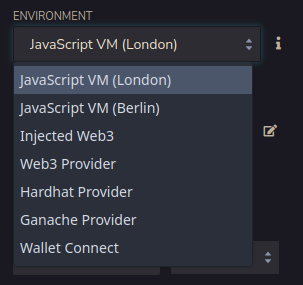
\includegraphics[width=0.4\textwidth]{Figures/remix.png}
    \caption{Posibles conexiones de Remix.}
    \cite{web:remix}
    \label{fg:remix}
\end{figure}
Metamask, de manera predeterminada, se conectara a la red principal de Ethereum e integrará una variable especial en el objeto \verb|window| de nuestro navegador.
\begin{lstlisting}
    if (typeof window.ethereum !== 'undefined') {
        console.log('Metamask is installed!');
    }
\end{lstlisting}
De la siguiente manera, se puede comprobar si Metamask está instalado.
Como desarrollador, solamente se tiene que seleccionar una dirección local para empezar.
\subsection{Ganache}
Ganache permite generar redes \textit{blockchain} locales. Metamask se puede conectar a esta red e interactuar con ella.
\begin{lstlisting}
    ganache-cli -p 8545 --mnemonic 
    \" word desert grief seven feature sight 
    object message upon lesson boat praise \" 
    --networkId 1337 --db ganache/db -q
\end{lstlisting}
Con el siguiente comando, se puede establecer un puerto con \verb|-p 8545|, se puede asegurar la carga de las mismas cuentas estableciendo un nemotécnico e introduciendo el id de la red, la cual tiene que ser 1337 ya que es local. Por ultimo, establecer una ruta para guardar todos los datos de la red. Es decir, todos los bloques de la \textit{blockchain}.
\subsection{Control de versiones}
Para este proyecto, se ha seleccionado \verb|git| como aplicación de control de versiones y GitHub \ref{fg:github} como repositorio remoto. Como este proyecto es código abierto, se ha creado un repositorio público para poder mostrar todos los pasos de desarrollo. De esa manera queda expuestos todos los \textit{commits} (confirmaciones) asociados a \textit{sprints}. Este repositorio también es útil como expositor temporal. Cualquier persona puede ver el desarrollo y verificar la integridad de nuestra solución.
\begin{figure}[h!]
    \centering
    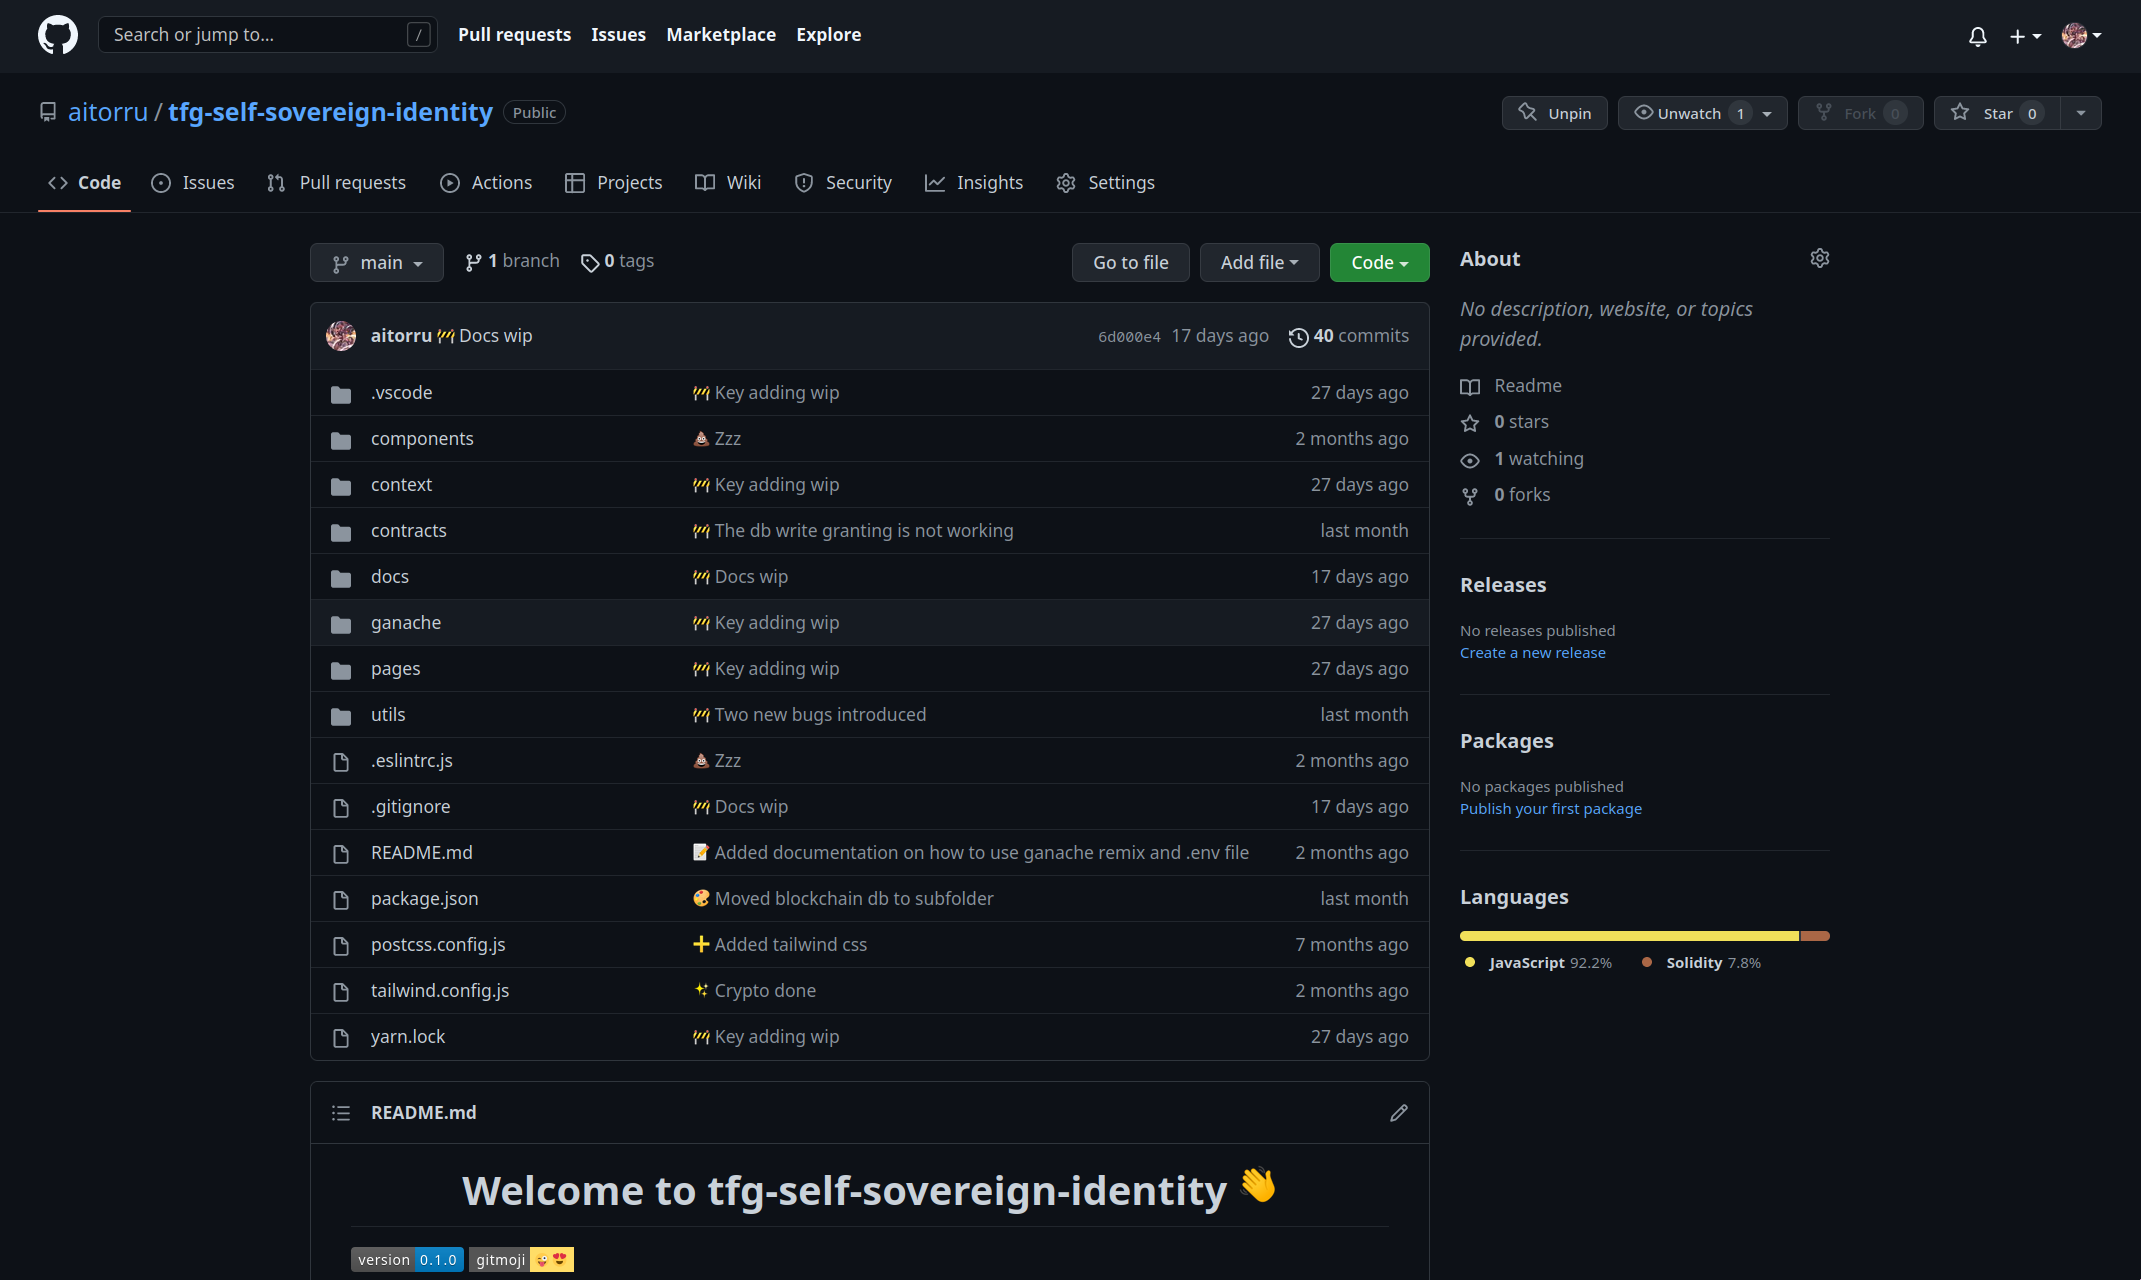
\includegraphics[width=0.8\textwidth]{Figures/github.png}
    \caption{Repositorio de github del proyecto}
    \label{fg:github}
    \cite{web:repo}
\end{figure}
\subsection{Contexto}
Para una planificación de temas, se usó una herramienta diferente. En vez de utilizar un fichero o una nota en \verb|notion.so|, se decidió utilizar apuntes en el código. Como se tenia acceso a los objetivos desde el inicio del desarrollo, se podían crear funciones vacías a modo de punto de inicio. Después se pueden crear comentarios para generar contexto.
\begin{lstlisting}
    // TODO: Hacer funcionar el proyecto
    // FIXME: El reloj no devuelve el tiempo en ISO
\end{lstlisting}
Todos los IDEs tienen la capacidad de generar árboles de \verb|TODOs| (por hacer) y \verb|FIXMEs| (arreglar). En \verb|Code - OSS| \cite{web:code-oss}, un clon de código abierto de \verb|vscode|, existen extensiones para facilitar el proyecto.
De esta manera, los comentarios \ref{fg:todoTree} sirven como herramienta de contexto a lo largo de un \textit{sprint}.
\begin{figure}[H]
    \centering
    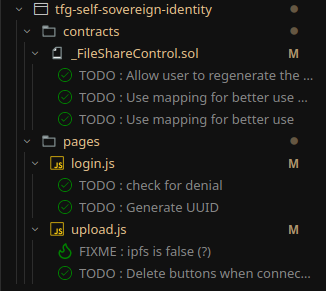
\includegraphics[width=0.5\textwidth]{Figures/TodoTree.png}
    \caption{Ejemplo de visualización de comentarios}
    \label{fg:todoTree}
\end{figure}
\section{Herramientas utilizadas}
A continuación se procederá a detallar y a analizar las herramientas utilizadas para el funcionamiento de este PFG. Las herramientas de desarrollo estarán especificadas en el apartado de metodología \ref{Metodología}.
\subsection{React}
\verb|React| es una buena opción para crear UI \textit{responsivas} y fácilmente actualizables. Como en este proyecto se están escuchando eventos de la red y actualizando todo constantemente, utilizar este \textit{framework} es una gran opción. \verb|React| nos ofrece \textit{hooks} para actualizar la interfaz del usuario. 
En los siguientes puntos del proyecto se explicará con detalle el uso de React en esta aplicación.
\subsection{Metamask}
Metamask es un \textit{wallet} (cartera) que se puede comunicar con la \textit{blockchain} de Ethereum, la cual dispone de funcionalidades de firma, encriptación y desencriptación muy útiles para este proyecto. Existe como una extensión en el navegador y también tiene la capacidad de usarse desde el dispositivo móvil.
\subsection{OrbitDB}
OrbitDB es una base de datos distribuida. Ha sido construida por encima de \verb|js-ipfs| (una librería que convierte nuestro navegador en un nodo de IPFS). Utiliza su sistema de \textit{peers} para poder compartir datos utilizando una ruta a la que se puede acceder. Gracias a la criptografía, se pueden implementar permisos de lectura y escritura. La información de la base de datos se guarda en el \verb|local storage| del navegador. El funcionamiento es totalmente nuevo dentro de los paradigmas actuales, principalmente por la naturaleza inmutable de IPFS. La dirección de una base de datos hace referencia a un fichero en IPFS.\\
\verb|/OrbitDB/Qmd8TmZrWASypEp4Er9tgWP4kCNQnW4ncSnvjvyHQ3EVSU/database-name|\\
Esta URL contiene las siguientes partes.
\begin{itemize}
    \item \textbf{OrbitDB}: hace referencia a que el fichero existe en una carpeta llamada OrbitDB. Esto se hace por simplicidad. Todos los proyectos introducen sus datos bajo las carpetas de su organización para poder saber a quien pertenecen.
    \item \textbf{Qmd8TmZrWASypEp4Er9tgWP4kCNQnW4ncSnvjvyHQ3EVSU}: esta sección es generada aleatoriamente, sobre todo para evitar conflictos. Esto genera un problema, ya que al ser aleatorio no podemos saber cual es la base de datos de nuestro del \textit{peer} al que queremos contactar. Este problema se solucionará más adelante en el proyecto.
    \item \textbf{database-name}: este último apartado es libre. Esto significa que como ya hemos evitado conflictos entre bases de datos, se puede aportar un nombre útil para la aplicación. En el caso de este proyecto, se utiliza la dirección de la \textit{wallet} del usuario.
\end{itemize}
En esta dirección hay un archivo que solamente tiene la clave publica de OrbitDB. De este modo, todos los usuarios que se quieran conectar pueden leer la clave con la seguridad de que no ha sido manipulada.
\begin{figure}[H]
    \centering
    \includegraphics[width=0.7\textwidth]{Figures/OrbitDB.png}
    \caption[Diagrama básico de conexión de OrbitDB]{Diagrama que ejemplifica una base de datos compartida en el que el nodo propietario es el verde.}
    \label{fg:orbit}
\end{figure}
En el siguiente escenario \ref{fg:orbit}, hay una serie de nodos escuchando al nodo con la clave pública que han podido obtener del fichero. Al mismo tiempo, todos escuchan al mismo \textit{topic} que han obtenido desde el fichero.
\begin{figure}[h!]
    \centering
    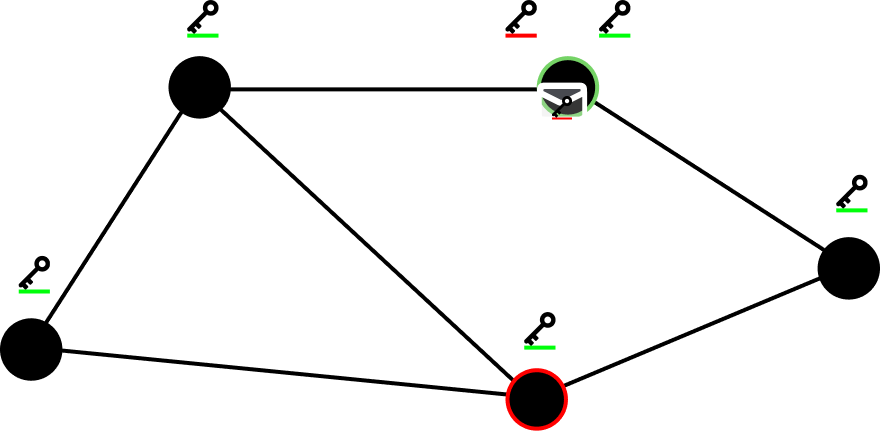
\includegraphics[width=0.7\textwidth]{Figures/Message sent.png}
    \caption{El nodo verde envía un mensaje.}
    \label{fg:messageSent}
\end{figure}
\begin{figure}[h!]
    \centering
    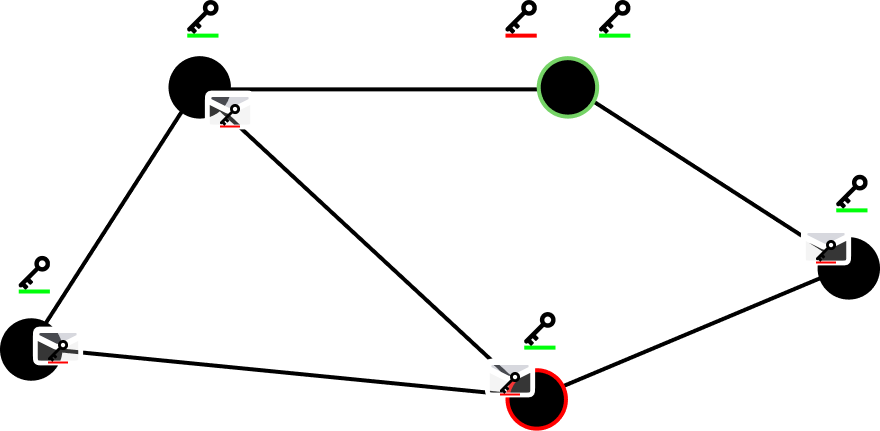
\includegraphics[width=0.7\textwidth]{Figures/Message arived.png}
    \caption{El resto de la red recibe el mensaje}
    \label{fg:messageRecived}
\end{figure}
Los mensajes salen del \textit{host} verde firmados con su clave privada \ref{fg:messageSent}. Utilizando la clave publica del \textit{host} verde (que han obtenido de la dirección original de IPFS) pueden verificar la legitimidad del origen y actualizar su copia de la base de datos \ref{fg:messageRecived}.
\begin{figure}[h!]
    \centering
    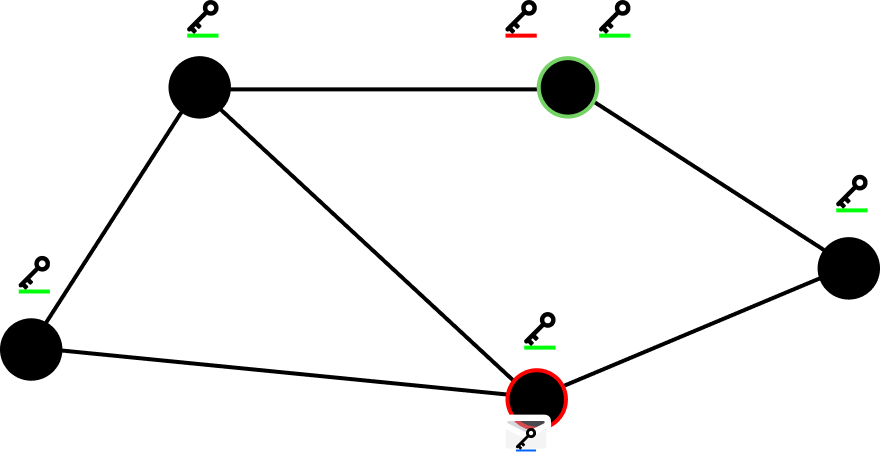
\includegraphics[width=0.7\textwidth]{Figures/Message is compromissed.png}
    \caption{El nodo rojo intenta sobrescribir la información de los nodos}
    \label{fg:messageSentRed}
\end{figure}
\begin{figure}[h!]
    \centering
    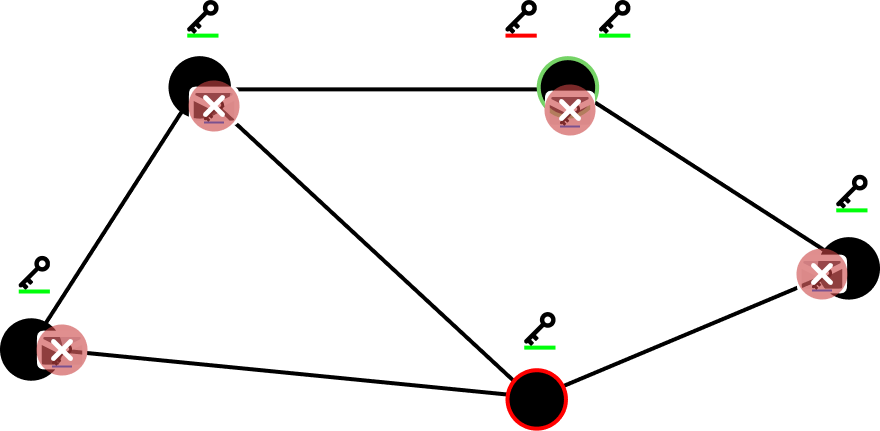
\includegraphics[width=0.7\textwidth]{Figures/Message rejected.png}
    \caption{El resto de la red rechaza el mensaje, ya que la clave no se puede verificar}
\end{figure}
\newpage
\thispagestyle{empty}
\chapter{Proceso de software ejecutado}\label{Proceso de software ejecutado}
%Función que crea el título de capítulo y al cual se le da el nombre deseado a través de su parámetro obligatorio. Al no tener la función el “*” se escribirá también en el título del documento las palabras “Capítulo 1: …”. Además se indica, mediante la función “\label”, la correspondiente etiqueta que lleva asociada. La etiqueta sirve para que en caso de que luego se quiera hacer referencia al capítulo se haga llamando etiqueta tal que se escribiría “La información correspondiente a dicho tema se encuentra en el capítulo \ref{Int}.”

\thispagestyle{fancy}
%Función que determina que durante este capítulo se aplique el estilo Fancy.

\fancyhead[LE]{\thechapter.Proceso de software ejecutado} 
%Función que se utiliza para indicar que en las páginas impares, aparezca en el encabezado en la parte izquierda, el número del capítulo con su correspondiente nombre.

En este capitulo, se va a explorar los requisitos del proyecto, el diseño seguido para cumplirlo, el desarrollo para poner en practica la idea y por ultimo la validación para comprobar su funcionamiento.

\section{Análisis}
Para poder resolver los problemas de identidad del mundo, hay que crear una lista de requisitos. Después de realizar nuestro desarrollo, se volverá a visitar la lista para concluir si nuestro desarrollo ha sido satisfactorio.

\subsection{Requisitos (funcionales y no funcionales)}
Antes de comenzar a desarrollar la solución, hay que analizar las posibilidades y elegir las librerías correctas.

\definecolor{Gray}{gray}{0.9}

\begin{center}
    \begin{table}[h!]
        \begin{tabular}{|p{0.1\linewidth} | p{0.8\linewidth}|}
            \hline
            \rowcolor{Gray} 
            \textbf{O1} & \textbf{Diseño de un sistema de SSI distribuido.} \\
            \hline
            RF1         & La plataforma debe contar con una pagina web estática. \\
            \hline
            RF2         & La plataforma debe poder enviar datos en un medio distribuido. \\
            \hline
            RF3         & La plataforma debe comunicarse con una red blockchain. \\
            \hline
            RF4         & La plataforma debe poder identificar usuarios en un mundo medio distribuido. \\
            \hline
            RF5         & La plataforma debe procesar peticiones de los usuarios en un medio distribuido. \\
            \hline
            RNF1        & La plataforma debe ser \textit{open source}. \\
            \hline
            RNF2        & La plataforma debe usar librerías \textit{open source}. \\
            \hline
        \end{tabular}
    \end{table}
\end{center}
\textbf{La plataforma debe contar con una pagina web estática.}\\
Para poder desplegar nuestra aplicación web en IPFS \cite{web:ipfs}, necesitamos que nuestra página sea estática. Esto significa que no podemos generar nuestro HTML en un servidor.
\begin{center}
    \begin{table}[h!]
        \begin{tabular}{|p{0.1\linewidth} | p{0.8\linewidth}|}
            \hline
            \rowcolor{Gray} 
            \textbf{O1-RF1} & \textbf{La plataforma debe contar con una pagina web estática.} \\
            \hline
            S111            & Empaquetado de \textit{assets}. \\
            \hline
            S112            & Optimización de código. \\
            \hline
            S113            & \textit{Code splitting.} \\
            \hline
        \end{tabular}
    \end{table}
\end{center}
\begin{itemize}
    \item \textbf{S111}: La herramienta, debe tener una opción para poder empaquetar HTML, JS y CSS en un solo fichero JS.
    \item \textbf{S112}: La herramienta, debe optimizar nuestra aplicación para que tenga un mejor rendimiento.
    \item \textbf{S113}: La herramienta, debe poder dividir nuestro payload en diferentes ficheros para no tener que enviar un archivo excesivamente grande.
\end{itemize}
\textbf{La plataforma debe poder enviar datos en un medio distribuido.}\\
Ya que se quiere implementar un sistema de identidades distribuidas, necesitaremos un canal por el que poder comunicar a todos los usuarios.
\begin{center}
    \begin{table}[h!]
        \begin{tabular}{|p{0.1\linewidth} | p{0.8\linewidth}|}
            \hline
            \rowcolor{Gray} 
            \textbf{O1-RF2} & \textbf{La plataforma debe poder enviar datos en un medio distribuido.} \\
            \hline
            S121            & Capacidad de mutar datos. \\
            \hline
            S112            & Seguro. \\
            \hline
        \end{tabular}
    \end{table}
\end{center}
\begin{itemize}
    \item \textbf{S121}: La herramienta, tiene que ser capaz de proporcionar las herramientas necesarias de mutar datos. Este paso es esencial si se necesita implementar una base de datos.
    \item \textbf{S122}: La herramienta, tiene que poder asegurarnos que el transporte de los datos es seguro entre nodos para evitar la suplantación de identidad.
\end{itemize}
\textbf{La plataforma debe comunicarse con una red blockchain.}\\
Para poder verificar que el usuario es quien dice ser, necesitamos un medio que nos garantice la trazabilidad de las identidades sin revelar los datos personales de las mismas.
\begin{center}
    \begin{table}[h!]
        \begin{tabular}{|p{0.1\linewidth} | p{0.8\linewidth}|}
            \hline
            \rowcolor{Gray} 
            \textbf{O1-RF3} & \textbf{La plataforma debe comunicarse con una red blockchain.} \\
            \hline
            S131            & Exponer un método de comunicación desde la interfaz. \\
            \hline
            S132            & Compatible con librerías de escucha a contratos. \\
            \hline
        \end{tabular}
    \end{table}
\end{center}
\begin{itemize}
    \item \textbf{S131}: La herramienta, tiene que exponer un puerto de comunicación desde el que se pueda enviar y recibir información.
    \item \textbf{S132}: La herramienta, tiene que ser compatible con librerías de escucha a contratos para poder responder a eventos que ocurran.
\end{itemize}
\textbf{La plataforma debe poder identificar usuarios en un mundo medio distribuido.}\\
A fecha de publicación de este trabajo, la web todavía no dispone de un estándar para las identidades distribuidas. Aún así, existe una propuesta en camino de ser aceptada \cite{web:did-spec}.
\begin{center}
    \begin{table}[h!]
        \begin{tabular}{|p{0.1\linewidth} | p{0.8\linewidth}|}
            \hline
            \rowcolor{Gray} 
            \textbf{O1-RF4} & \textbf{La plataforma debe poder identificar usuarios en un mundo medio distribuido.} \\
            \hline
            S141            & Decodificar DID. \\
            \hline
            S142            & Codificar DID. \\
            \hline
        \end{tabular}
    \end{table}
\end{center}
\begin{itemize}
    \item \textbf{S141}: La herramienta, debe ser capaz de decodificar los DID y obtener la información necesaria.
    \item \textbf{S142}: La herramienta, debe ser capaz de codificar el DID del usuario accediendo a su cartera.
\end{itemize}
\textbf{La plataforma debe procesar peticiones de los usuarios en un medio distribuido.}\\
Al no disponer de un backend, tenemos que diseñar una alternativa para conseguir la misma funcionalidad utilizando el mundo distribuido. En vez de usar un patrón de diseño REST, se va a utilizar gRCP. Esto se debe a que nuestro backend, no tiene datos los cuales puede devolver. Solo podemos ejecutar funciones.
\begin{center}
    \begin{table}[h!]
        \begin{tabular}{|p{0.1\linewidth} | p{0.8\linewidth}|}
            \hline
            \rowcolor{Gray}
            \textbf{O1-RF5} & \textbf{La plataforma debe procesar peticiones de los usuarios en un medio distribuido.} \\
            \hline
            S151            & Exponer funciones para ser llamadas desde los usuarios. \\
            \hline
        \end{tabular}
    \end{table}
\end{center}
\begin{itemize}
    \item \textbf{S151}: Siguiendo un patrón gRCP, se expondrán funciones con las se podrán llamar desde la aplicación.
\end{itemize}
\textbf{La plataforma debe ser \textit{open source}.}\\
Para asegurar un desarrollo ético de este proyecto, se desarrollará bajo una licencia open source. Más adelante se explicarán las implicaciones éticas de este proyecto.
\begin{center}
    \begin{table}[h!]
        \begin{tabular}{|p{0.15\linewidth} | p{0.75\linewidth}|}
            \hline
            \rowcolor{Gray} 
            \textbf{O1-RNF1} & \textbf{La plataforma debe ser \textit{open source}.} \\
            \hline
            S11N1            & Licencia \textit{open source}. \\
            \hline
        \end{tabular}
    \end{table}
\end{center}
\begin{itemize}
    \item \textbf{S11N1}: Para asegurar que el proyecto y los próximos que avancen lo creado en este, se usará una licencia que lo pueda asegurar. \textbf{GNU General Public License v3.0}.
    \begin{table}[h!]
        \centering
        \begin{tabular}{|c|c|c|}
            \hline
            Permissions         & Limitations   & Conditions \\
            \hline
            Commercial use      & Liability     & License and copyright notice \\
            \hline
            Modification        & Warranty      & State changes \\
            \hline
            Distribution        &               & Disclose source\\
            \hline
            Patent use          &               & Same license \\
            \hline
            Private use         &               & \\
            \hline
        \end{tabular}
        \cite{web:LICENSE}
    \end{table}
\end{itemize}
\textbf{La plataforma debe usar librerías open source.}
Este proyecto, al ser open source, utilizará multiples librerías, todas ellas de código abierto. De esa manera, cualquier fragmento de código puede ser verificado.
\begin{center}
    \begin{table}[h!]
        \begin{tabular}{|p{0.15\linewidth} | p{0.75\linewidth}|}
            \hline
            \rowcolor{Gray} 
            \textbf{O1-RNF2} & \textbf{La plataforma debe usar librerías \textit{open source}.} \\
            \hline
            S11N2            & Licencia \textit{open source}. \\
            \hline
        \end{tabular}
    \end{table}
\end{center}
\begin{itemize}
    \item \textbf{S12N1}: Las librerías usadas deberán usar licencias de código abierto.
\end{itemize}
\noindent\rule{\textwidth}{0.4pt}
\newpage
\begin{center}
    \begin{table}[h!]
        \begin{tabular}{|p{0.1\linewidth} | p{0.8\linewidth}|}
            \hline
            \rowcolor{Gray} 
            \textbf{O2} & \textbf{Desarrollo de un sistema de SSI distribuido.} \\
            \hline
            RF1     & La plataforma debe ejecutar un nodo IPFS \cite{web:ipfs}. \\
            \hline
            RF2     & La plataforma debe contar con las APIs necesarias para comunicarse con la cartera del usuario.\\
            \hline
            RF3     & La plataforma debe ejecutar una base de datos orbit db. \\
            \hline
        \end{tabular}
    \end{table}
\end{center}
\textbf{La plataforma debe ejecutar un nodo IPFS \cite{web:ipfs}.}\\
Como la herramienta elegida ha sido IPFS \cite{web:ipfs}, se necesitará asegurar su correcto funcionamiento.
\begin{center}
    \begin{table}[h!]
        \begin{tabular}{|p{0.15\linewidth} | p{0.75\linewidth}|}
            \hline
            \rowcolor{Gray} 
            \textbf{O2-RF1} & \textbf{La plataforma debe ejecutar un nodo IPFS \cite{web:ipfs}.} \\
            \hline
            S211     & Configuración correcta con servidores star. \\
            \hline
            S212     & Configuración correcta de orbit db. \\
            \hline
            S213     & Generar métodos para descargar datos y desencriptarlos. \\
            \hline
            S214     & Generar métodos para subir datos y encriptarlos. \\
            \hline
        \end{tabular}
    \end{table}
\end{center}
\begin{itemize}
    \item \textbf{S211}: Se deberá configurar IPFS \cite{web:ipfs} correctamente para que los usuarios se puedan encontrar entre ellos.
    \item \textbf{S212}: Para que las bases de datos se puedan replicar correctamente, orbit db necesita estar configurado correctamente.
    \item \textbf{S213}: Para poder subir información a IPFS \cite{web:ipfs}, necesitaremos que esté encriptada para la seguridad del usuario.
    \item \textbf{S214}: Para descargar información de IPFS \cite{web:ipfs}, necesitaremos desencriptarlos.
\end{itemize}
\textbf{La plataforma debe contar con las APIs necesarias para comunicarse con la cartera del usuario.}\\
Para poder comunicarnos con la cartera necesitaremos utilizar el objeto \verb|window.ethereum| correctamente.
\begin{center}
    \begin{table}[h!]
        \begin{tabular}{|p{0.15\linewidth} | p{0.75\linewidth}|}
            \hline
            \rowcolor{Gray} 
            \textbf{O2-RF2} & \textbf{La plataforma debe contar con las APIs necesarias para comunicarse con la cartera del usuario.} \\
            \hline
            S221     & Métodos auxiliares para usar la funcionalidad de la cartera \\
            \hline
        \end{tabular}
    \end{table}
\end{center}
\begin{itemize}
    \item \textbf{S221}: Se crearán métodos generalistas para poder comunicarse con metamask.
\end{itemize}
\textbf{La plataforma debe ejecutar una base de datos orbit db.}\\
Para poder ejecutar una base de datos, se necesitará crear una instancia de IPFS \cite{web:ipfs}.
\begin{center}
    \begin{table}[h!]
        \begin{tabular}{|p{0.15\linewidth} | p{0.75\linewidth}|}
            \hline
            \rowcolor{Gray} 
            \textbf{O2-RF3} & \textbf{La plataforma debe contar con las APIs necesarias para comunicarse con la cartera del usuario.} \\
            \hline
            S231     & Generar claves para la comunicación. \\
            \hline
            S232     & Generar base de datos \textit{keyvalue}. \\
            \hline
            S233     & Generar métodos de escucha de eventos. \\
            \hline
            S234     & Subir DID a la base de datos. \\
            \hline
        \end{tabular}
    \end{table}
\end{center}
\begin{itemize}
    \item \textbf{S231}: Para poder iniciar la comunicación, necesitaremos generar las claves publica y privada.
    \item \textbf{S232}: Se necesitará crear una base de datos \textit{keyvalue}.
    \item \textbf{S233}: Para poder avisar al usuario de lo que ocurra, hay que poder escuchar a eventos en la red.
    \item \textbf{S234}: Para presentar al usuario ante el resto, habrá que subir nuestra identificación a la base de datos.
\end{itemize}
\section{Diseño}
En este apartado, se va a diseñar la solución para poder cumplir los requisitos del sistema.
\subsection{Arquitectura general}
\begin{figure}[h!]
    \centering
    \includegraphics[width=0.9\textwidth]{Figures/Diseño.png}
    \caption{Diseño de la aplicación. Los nodos color verde son puertos de escucha IPFS \cite{web:ipfs}. El nodo de color naranja es un puerto de escucha de MetaMask.}
\end{figure}
Este es el diseño actual de la solución. \textit{A priori}, parece imposible que pueda funcionar ya que no existe ningún tipo de \textit{backend} en el que podamos ejecutar la lógica. Toda la lógica se ejecuta utilizando \textit{smart contracts} y el resto son intercambios de datos por IPFS \cite{web:ipfs}.
La conexión de metamask con la blockchain esta fuera del área de control. Para poder interactuar con la cartera, disponemos de un canal de comunicación en el que podemos enviar mensajes.
\begin{lstlisting}
    const syncKey = await window.ethereum.request({
			method: '',
			params: [],
    });
\end{lstlisting}
Utilizando esta función, podemos enviar un \verb|method|, y unos argumentos. Los métodos, son las funcionalidades que puede hacer metamask.
Por ejemplo, para poder compartir la identidad del usuario y empezar a trabajar, tenemos que pedirle permiso. 
\begin{lstlisting}
    let encryptionPublicKey;
    ethereum
    .request({
        method: 'eth_getEncryptionPublicKey',
        params: [account], 
        // you must have access to the specified account
    })
    .then((result) => {
        encryptionPublicKey = result;
    })
    .catch((error) => {
        if (error.code === 4001) {
        // EIP-1193 userRejectedRequest error
        console.log("We can't encrypt anything without the key.");
        } else {
        console.error(error);
        }
    });
\end{lstlisting}
\cite{web:metamask_wiki}
\subsection{Modelo funcional}
A diferencia de otros frameworks clásicos que utilizan el modelo MVC (Model, View, Controller), Nextjs, aunque capaz de hacer renderizado por servidor, su función principal es generar paginas estáticas. Estas paginas, para ser renderizadas, son llamadas como una función. React, como ya se ha dicho antes, utiliza JSX, siendo capaz de añadir HTML en JS.
\begin{lstlisting}
    import Header from '../components/header';
    import HeroSection from '../components/hero';
    import Head from 'next/head';

    export default function Home() {
        return (
            <>
                <Head>
                    <title>TFG self soverign identity</title>
                    <meta name="viewport" content="initial-scale=1.0, width=device-width" />
                </Head>
                <Header />
                <HeroSection />
            </>
        );
    }
\end{lstlisting}
Para poder renderizar la pagina inicial (index), necesitamos ejecutar la función Home, que tiene un un return, que devuelve HTML.
Cuando un usuario solicita nuestra pagina, se le devuelve el HTML ya generado con el archivo JS que ha generado ese HTML en el servidor a la hora de construcción. El navegador, ejecuta ese archivo de JS hidratando la pagina y añadiendo toda la funcionalidad.
\subsection{Escucha de eventos}
\begin{figure}[h!]
    \centering
    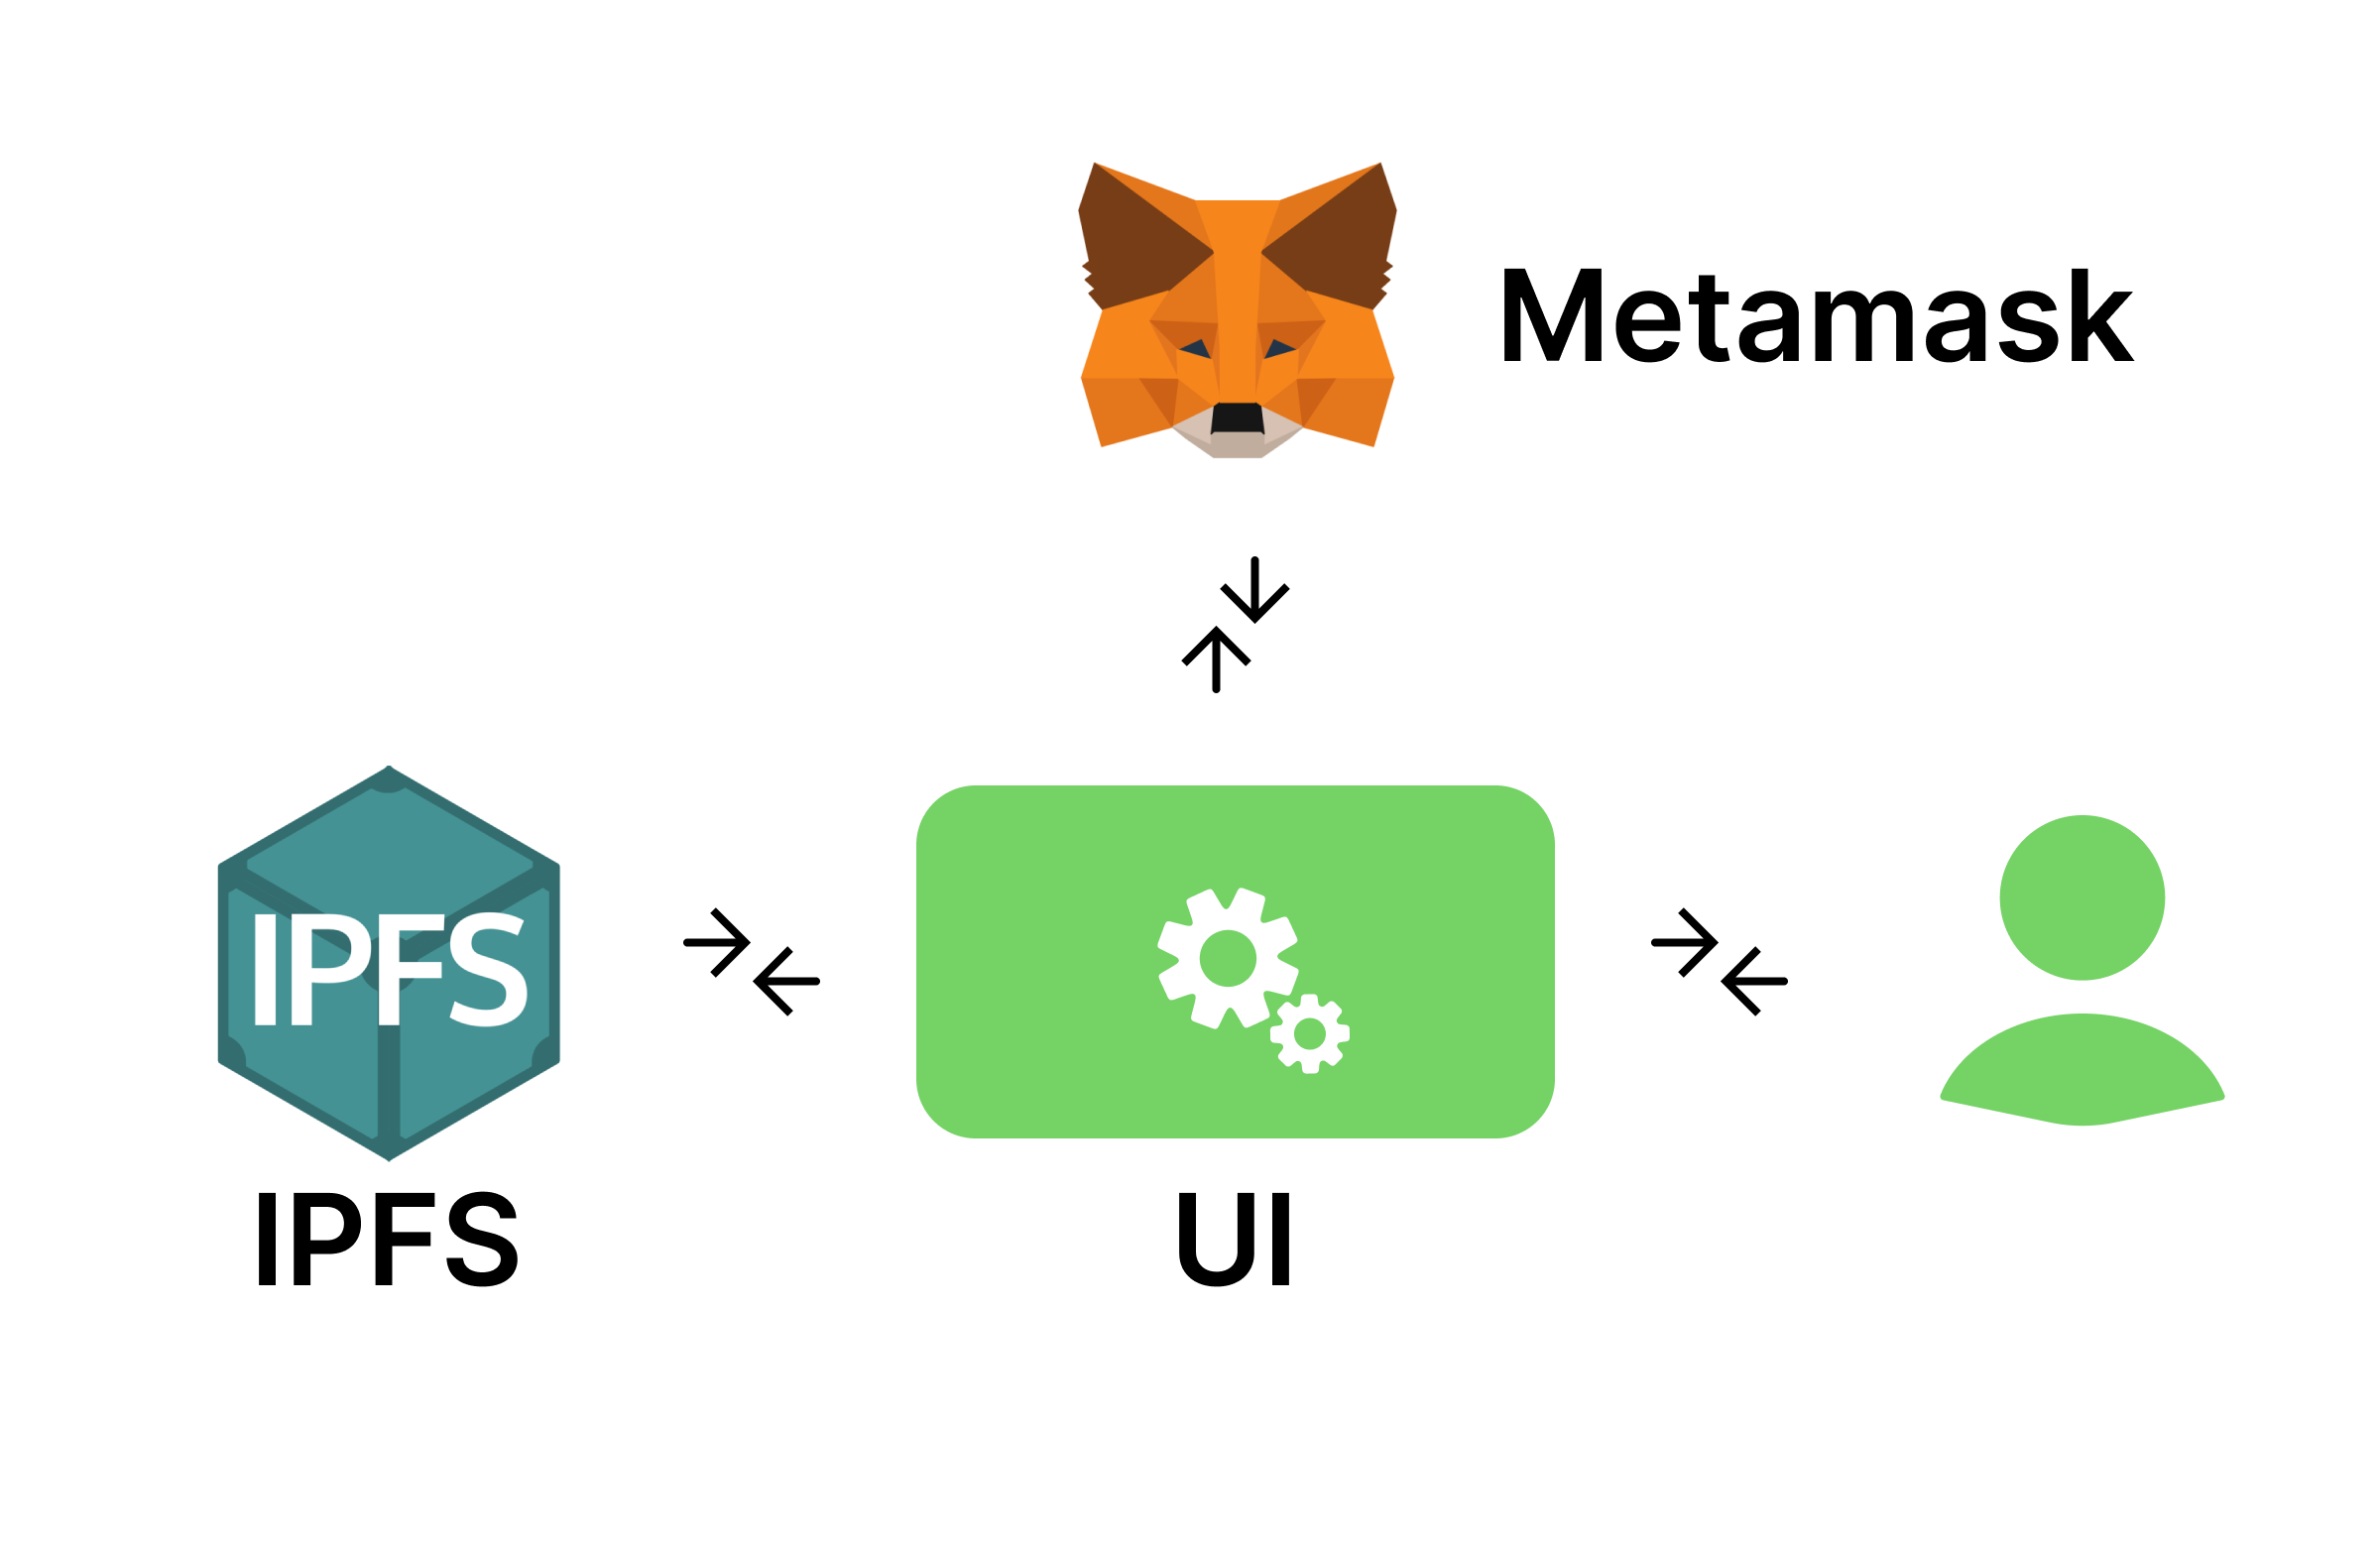
\includegraphics[width=0.9\textwidth]{Figures/Reactividad.png}
    \caption{Diagrama que muestra como la UI puede reaccionar a eventos que ocurren en la red para mostrar los cambios al ususario.}
\end{figure}
Este proyecto, una vez hidratado, es capaz de escuchar a eventos en la red. Gracias a esto, la UI es capaz de reaccionar y cambiar adecuadamente. Todo esto ocurriendo a tiempo real. Así mismo, también puede reaccionar a las acciones del usuario y reaccionar adecuadamente.
\subsection{Rutas}
Las rutas en nextjs, no son programáticas, sino contextuales. Las rutas se declaran creando archivos \verb|.js| en la carpeta pages.
\begin{lstlisting}
> tree
.
|-- _app.js
|-- index.js
|-- login.js
|-- upload.js

0 directories, 4 files
\end{lstlisting}
Este árbol, nos dice que hay tres rutas más un fichero con funcionalidad especial.
\begin{itemize}
    \item \verb|index|
    \item \verb|login|
    \item \verb|upload|
\end{itemize}
El archivo \verb|_app|, es un archivo que \textit{configura} al resto de las rutas.
Como el método de \verb|index| se llama \verb|Home|, el HTML resultante quedaría así.
\begin{lstlisting}
    <App>
        <Home/>
    </App>
\end{lstlisting}
En el método \verb|App|, podemos introducir lógica que queremos que se ejecute en cada página, incluyendo también el HTML que queremos en cada una. En este lugar, podemos establecer la lógica necesaria para comunicarnos con la cartera del usuario y una manera para poder compartir estado global a lo largo de toda la aplicación.
De este modo, al tratarse de una SPA \cite{web:spa} (Single page application), podemos mantener esa conexión sin y guardar por ejemplo la dirección del usuario o la conexión IPFS \cite{web:ipfs}.
\section{Desarrollo}
En esta sección, se va a exponer el desarrollo del proyecto siguiendo las guías establecidas en la sección de diseño.
\subsection{Entorno de desarrollo}
El entorno elegido para el desarrollo, es un ordenado fijo con un sistema operativo UNIX-like \cite{web:unix-like}. Con la ultima version de node instalada. Este sistema operativo ha sido escogido, por varios motivos. Al ser un sistema operativo centrado en la terminal, la experiencia de desarrollo, es muy superior a la que windows puede ofrecer. Así mismo, al ser un sistema operativo de código abierto, concuerda con la filosofía de este proyecto.
Así mismo, el navegador principal en el que se han realizado todas las pruebas han sido en el navegador Firefox. El cual también es código abierto.
Este sistema operativo, en especifico, Arch Linux \cite{web:arch}, era conocido, por lo tanto se pudo comenzar a diseñar de inmediato.
Como administrador de paquetes, en vez de utilizar npm \cite{web:npm}, se ha decidió elegir yarn ya que consigue instalar los paquetes a una velocidad superior permitiendo desbloquear una calidad de desarrollo superior. Yarn, como npm, es un gestor de paquetes que lee el contenido de \verb|package.json| y descarga todas las dependencias en \verb|node_modules|.
\begin{lstlisting}
    "dependencies": {
	"@ethersproject/providers": "^5.5.3",
    "@metamask/eth-sig-util": "^4.0.0",
    "@web3-react/core": "^6.1.9",
    "@web3-react/injected-connector": "^6.0.7",
    "@web3-react/walletconnect-connector": "^6.2.10",
    "axios": "^0.26.1",
    "bcrypt": "^5.0.1",
    "eth-crypto": "^2.2.0",
    "ethereumjs-util": "^7.1.4",
    "ethr-did": "^2.2.0",
    "ethr-did-resolver": "^5.0.4",
    "file-saver": "^2.0.5",
    "ipfs": "^0.62.1",
    "next": "12.0.10",
    "orbit-db": "^0.28.3",
    "orbit-db-identity-provider": "^0.4.0",
    "react": "^17.0.2",
    "react-dom": "^17.0.2",
    "react-ipfs": "^0.3.1",
    "react-query": "^3.34.16",
    "secp256k1": "^4.0.3",
    "tweetnacl": "^1.0.3",
    "tweetnacl-util": "^0.15.1",
    "use-callback-ref": "^1.2.5",
    "uuid": "^8.3.2",
    "web3": "^1.7.0"
    },
    "devDependencies": {
    "autoprefixer": "^10.4.2",
    "concurrently": "^7.1.0",
    "eslint": "^8.9.0",
    "eslint-plugin-react": "^7.28.0",
    "postcss": "^8.4.6",
    "tailwindcss": "^3.0.22"
    }
\end{lstlisting}
Todas estas dependencias, son descargadas y analizadas para realizar la instalación más óptima.
Hay dos tipos de dependencias.
\begin{itemize}
    \item \textbf{Desarrollo}
    Las dependencias de desarrollo, son solo librerías que vamos a utilizar para desarrollar nuestra aplicación. Por ejemplo, \verb|eslint| \cite{web:eslint} es una librería que escanea nuestro estilo de código e intenta \textit{indentarlo} de la manera configurada.
    Por ejemplo, en el siguiente fragmento de código, tenemos un error de \textit{indentarlo}.
    \begin{lstlisting}
        export default function MainButton({ text }) {
            return (
                <button>{text}</button>
            );
        }
    \end{lstlisting}
    En cambio, después de ejecutar eslint, nuestro código pasa a tener una estructura correcta.
    \begin{lstlisting}
        export default function MainButton({ text }) {
            return (
                <button>{text}</button>
            );
        }
    \end{lstlisting}
    \item \textbf{Producción}
    Las librerías de producción, son las utilidades que se han ido mencionando hasta ahora. Todas ellas son fundamentales para el funcionamiento de esta aplicación.
\end{itemize}
\subsection{Aplicación web}
Como ya se ha indicado anteriormente, Next.js \cite{web:next.js} es el framework que se va a utilizar para la resolución de este proyecto.
La estructura de un proyecto en nextjs tiene la siguiente estructura.
\begin{lstlisting}
    > tree -I 'node_modules|docs'
    .
    |-- components
    |   |-- button
    |   |   |-- index.js
    |   |-- header
    |   |   |-- index.js
    |   |-- hero
    |   |   |-- index.js
    |   |-- seccondaryButton
    |   |   |-- index.js
    |   |-- uploadPlatform
    |       |-- index.js
    |-- context
    |   |-- index.js
    |-- contracts
    |   |-- _FileShareControl.sol
    |-- ganache
    |   |-- README.md
    |-- package.json
    |-- pages
    |   |-- _app.js
    |   |-- index.js
    |   |-- login.js
    |   |-- upload.js
    |-- postcss.config.js
    |-- README.md
    |-- tailwind.config.js
    |-- utils
    |   |-- consts.js
    |   |-- index.js
    |-- yarn.lock

    11 directories, 19 files
\end{lstlisting}
Esta configuración no es obligatoria en su totalidad. Los únicos campos obligatorios son los archivos \verb|.js| en el directorio \verb|pages|.
El resto de las carpetas son elegidas por su expresividad.
\begin{itemize}
    \item \verb|components|\\
    Esta carpeta, contiene los componentes utilizados para el funcionamiento.
    En otros \textit{frameworks}, utilizaríamos plantillas para poder crear vistas del modelo M\textbf{V}C. Este cambio de paradigma, nos hace pensar en piezas reutilizables. En este caso piezas que podemos volver a utilizar.
    \begin{figure}[h!]
        \centering
        
\includegraphics[width=0.9\textwidth]{Figures/Example UI.png}
        \caption{Interfaz de ejemplo para explicar un \textit{framework} basado en componentes.}
        \label{fg:ui}
    \end{figure}
    Si tomamos de ejemplo esta interfaz \ref{fg:ui}, vemos que tenemos el mismo botón repetido multiples veces. Seguramente, ese botón tenga funcionalidad diferente. Algunos pueden actuar de link y otros pueden mutar datos de la base de datos.
    Todo esto, haría que tengamos que crear multiples botones en HTML con funcionalidad especifica cada uno. En un sistema clásico MVC, la creación de funcionalidad para botones, se convierte en una tarea complicada.
    En cambio, en framework basado en componentes, resulta en una experiencia superior y mucho mas modular.
    \begin{lstlisting}
        function Bt({text, onClick}) {
            return <button className='bg-blue-500' onClick={onClick}>{text}</button>
        }

        export default function Hero({content}) {
            return (
                // ...
                {
                    content.forEach(row => {
                        <div className='flex justify-between gap-5 ...'>
                            <p>{row.content}</p>
                            <Bt text={row.action.text} onClick={row.action.action} />
                        </div>
                    })
                }
                // ...
            )
        }
    \end{lstlisting}
    Con este pequeño segmento de código, podemos generar una interfaz igual de funcional que un framework MVC pero con renderizado en cliente. Sin necesidad de tener un backend para leer una base de datos. Así mismo, nuestro controlador es el mismo navegador. Este interactúa con la blockchain y con IPFS a demanda del usuario.
\end{itemize}
\subsection{Contexto}
El contexto de nuestra aplicación, es un grupo de variables globales. Hay dos tipos de variables que se usan en este proyecto.
Las variables asíncronas y las síncronas.
\begin{itemize}
    \item Las variables asíncronas, exponen dos variables en un array. La primera es el propio valor establecido y la segunda es una función que sirve para guardar el estado. Cuando se llama a la función para cambiar el estado, se avisa a React para que actualizar la interfaz. Es muy parecido a el \textit{Data-driven rendering} \cite{web:ddr} de los videojuegos. Son variables a las que no se les espera que cambien el estado para continuar con su ejecución. Esto implica que si tenemos que usar ese valor actualizado, podemos tener condiciones de carrera.
    \begin{lstlisting}
        const [valor, introducirValor] = useState(1)
        //...
        console.log(valor)
        // 1
        introducirValor(2)
        console.log(valor)
        // 1 (stale)
    \end{lstlisting}
    Como podemos ver en este ejemplo, aunque hemos actualizado el valor, seguimos obteniendo el resultado incorrecto.
    \item Las variables síncronas, por otra parte, su valor esta disponible nada más su asignación. Así mismo, estas variables no provocan un renderizado. Estas variables, se comportan de una manera muy parecida a las variables clásicas de JavaScript.
    \begin{lstlisting}
        let valor = 1
        console.log(valor)
        // 1
        valor = 2
        console.log(valor)
        // 2
    \end{lstlisting}
    En react, utilizamos un hook para mejorar la experiencia de desarrollo. Aunque, a nivel practico, son idénticas.
    \begin{lstlisting}
        const valor = useRef(1)
        //...
        console.log(valor.current)
        // 1
        valor.current = 2
        console.log(valor.current)
        // 2
    \end{lstlisting}
    Como es aparente, el nombre de la variable viene continuado por \verb|.current|. Esto se explicará mas adelante.
\end{itemize}
\subsection{Base de datos}
Este proyecto difiere con todos los paradigmas actuales introduciendo una base de datos distribuida. Esta base de datos distribuida, se parece mucho a la blockchain, ya que todo el mundo tiene una copia de los datos que contiene.
Por ahora no existe una adaptación de una base de datos relación tipo relacional \cite{web:relational-database}. Solo existen los siguientes tipos:
\begin{itemize}
    \item \textbf{Log}\\
    Un registro de solo entrada con la capacidad de explorar el historial. Útil cuando se quiere saber la ultima entrada.
    \item \textbf{Feed}\\
    A diferencia del anterior, en este tipo de base de datos si que se pueden mutar los datos. Este tipo de base de datos es útil para un uso parecido a un carrito de la compra.
    \item \textbf{Key Value}\\
    Este tipo de base de datos funciona exactamente igual que la búsqueda en redis \cite{web:redis}. También se puede  comparar con el funcionamiento de un \textit{Hash map} \cite{web:hash-table}.
    \item \textbf{Docs} \\
    Implementación minima de una base de datos documental. Los archivos se consideran documentos a los cuales se puede acceder por su nombre. Parecido a MongoDB \cite{web:mongodb} pero más limitado.
    \item \textbf{Counter} \\
    Útil para contar eventos de manera separada a el Log o el Feed.
\end{itemize}
\subsection{Key Value}
La base de datos utilizada para este proyecto ha sido la \textbf{key value} ya que se pueden asignar datos a direcciones de la cartera de cada usuario.
En el mundo distribuido, cada persona tiene su base de datos, pero es dependiente a el dominio al que pertenece. Eso quiere que si viene un usuario nuevo, hay que generar su DID \cite{web:did}.
Para poder comenzar a compartir información, hay que conectarse o crear una base de datos. Como se ha dicho anteriormente, todos los conectados a una base de datos comparten la misma información. Eso significa que a niveles prácticos todos los usuarios que estén conectados entre si en la misma sala compartirán base de datos entre ellos.
Las salas, son las propias aplicaciones. Una sala puede ser desde alud a un twitter descentralizado.
Como estamos todos conectados, si el usuario \textbf{0xc0ffee254729296a45a3885639AC7E10F9d549} quiere obtener la clave publica del usuario \textbf{0x70E3Aed5aA1aac6EC39D114B7411DF6f1CC80671}, simplemente tiene que buscar su entrada en la base de datos.
\subsection{Permisos}
Para poder entrar a una sala, se necesitan permisos. Por la misma razón que actualmente se necesita un usuario y contraseña para entrar en la mayoría de las paginas de internet, en el mundo distribuido ocurre lo mismo.
Cuando se crea una base de datos se pueden asignar dos tipos de permisos.
\begin{itemize}
    \item \textbf{Publica}\\
    A la hora de generar la base de datos se puede especificar un *. Esto significa que cualquier identificador puede escribir.
    \begin{lstlisting}
        let options = {
			// Give write access to yourself at first
			accessController: {
				write: [
					*,
				],
			},
		};
    \end{lstlisting}
    \item \textbf{Privada}\\
    Para nuestra aplicación y generalmente para cualquier uso serio de esta tecnología, las bases de datos deben ser permisionadas.
    \begin{lstlisting}
        let options = {
			// Give write access to yourself at first
			accessController: {
				write: [
					orbitdb.identity.id,
				],
			},
		};
    \end{lstlisting}
\end{itemize}
El objeto \verb|orbitdb.identity.id|, es el identificador del creador. Es como la matricula de nuestro coche. Un justificante criptográfico que permite la aceptación de mensajes dependiendo de si el origen es correcto o no. De este modo evitando maneras de sobrescribir datos.
\subsection{Smart contract}
Para poder aceptar a personas en nuestra sala, necesitamos una forma de identificar a personas y verificar que proceden de quien dicen ser. Si implementamos una base de datos publica en la que cualquier personas puede introducir sus credenciales, alguien con peores intenciones que nosotros, puede sobre-escribirlas consiguiendo robar información.
En cambio, introduciendo la tecnología blockchain, podemos utilizar todas sus posibilidades criptográficas para verificar que el origen es verídico.
En esta aplicación, cualquier persona puede crear una sala y cualquier otra persona solicitar unirse. Como la blockchain es un registro total de todas las transacciones, siempre tenemos un registro de que salas han sido creadas y si alguien ha querido entrar mientras no estábamos escuchando.
\begin{lstlisting}
// SPDX-License-Identifier: GPL-3.0

pragma solidity >=0.7.0 <0.9.0;

/**
 * @title FileShareControl
 * @dev Publish and allow users into your db
 */
contract FileShareControl {
    struct Room {
        address owner;
        string orbit_db_url;
    }
    mapping (address => Room) rooms;
    // TODO: Use mapping for better use
    struct Proposal {
        address proposer;
        address proposalTo;
        string orbit_db_identity;
        bool accepted;
    }
    mapping (address => Proposal) proposals;

    // Declare events. Will be used in js 
    event RoomCreated(address owner, string url);
    event ProposalCreated(address owner, address proposer, string identity);
    event ProposalAccepted(address proposer, string url);

    function createRoom(string memory url) 
    public 
    {
        // We cannot use "rooms[address] = Room(0x00000...0, "...")"
        // because the right hand side creates a memory-struct "Room" that contains a mapping
        Room storage r      = rooms[msg.sender];
        r.owner             = msg.sender;
        r.orbit_db_url      = url;
        emit RoomCreated(msg.sender, url);
    }

    function createProposal(address proposalTo, string memory identity)
        public
    {
        Proposal storage p  = proposals[msg.sender];
        p.proposer          = msg.sender;
        p.proposalTo        = proposalTo;
        p.orbit_db_identity = identity;
        emit ProposalCreated(proposalTo, msg.sender, identity);
    }

    function acceptProposal(address proposer) 
    public 
    {
        // First get the origin room
        Room memory r = rooms[msg.sender];
        // Check if the room exists. If not, the struct is generated with default values.
        // Default value of address
        require(r.owner != 0x0000000000000000000000000000000000000000, "You don't have any room.");
        
        Proposal memory p = proposals[proposer];
        // Proposal checks
        require(p.proposer !=  0x0000000000000000000000000000000000000000 && p.proposalTo != 0x0000000000000000000000000000000000000000, "The proposal doesn't exists.");
        require(p.proposalTo == msg.sender, "You are not the origin");
        require(p.proposer == proposer, "(+_+)");
        require(!(p.accepted), "The proposal is already accepted");
        // Warn the proposer that he is accepted
        emit ProposalAccepted(proposer, r.orbit_db_url);
    }

}
\end{lstlisting}
Se divide en tres métodos principales que son usados a la hora de verificación.
\begin{itemize}
    \item \verb|createRoom|, anuncia la creación de una sala para que el resto de la red sepa de su existencia.
    Esta sala tiene una URL que pertenece a la dirección de escucha de orbit db.
    \item \verb|createProposal|, crea una petición para entrar a una sala.
    Para poder entrar, hay que avisar al creador que queremos entrar en su sala y adjuntamos nuestra matricula de orbit db para que se adjunte a la lista con permisos de escritura.
    \item \verb|acceptProposal|, acepta la solicitud. Este método, es solo una manera de avisar correctamente al solicitante de que puede entrar. No muy útil cuando el usuario esta conectado a la pagina directamente porque se podrían usar métodos tradicionales, sino porque al ser un registro histórico, también podría entrar en las siguientes ocasiones sin tener que quemar más gas.
\end{itemize}
\subsection{Eventos - Orbit db y Ethereum}
Como ya se ha comentado anteriormente, nuestra interfaz tiene que ser capaz de responder a eventos de la red. Tanto por parte de IPFS como por parte de Ethereum.
Las librerías web 3.0 nos ayudan a realizar esta tarea de una manera mas eficaz. De todas formas, podemos encontrarnos con multiples problemas.
La escucha de eventos, se carga al inicio de la aplicación. Esto significa que la primera vez que JS hidrata la pagina y nuestro JS es montado. Es decir, nuestra función es llamada, se ejecutan nuestras funciones de escucha.
Para poder escuchar a eventos, generalmente se suelen usar las callbacks. Callback en español significa “llamada de vuelta”. Esto significa que si ocurre algo nos avisaran llamándonos de vuelta.
Esto se puede conseguir ya que en JavaScript, permite asignar como valor de una variable una función.
\begin{lstlisting}
    const functionInsideAvar = () => { return 1 + 1 }
\end{lstlisting}
Si llamamos a esta variable, nos devolverá la suma de \verb|1 + 1|, \verb|2|.
Esta función es relativamente \verb|inútil|, ya que no estamos aprovechando las posibilidades de los callbacks.
\begin{lstlisting}
    cosnt msghandler = (msg) => {console.log(msg)}

    msghandler('primero')
    msghandler('segundo')
\end{lstlisting}
Como podemos apreciar en este ejemplo, podemos pasar contenido a la función. Eso nos abre muchísimo las posibilidades.  Estas funciones nos permiten que el framework solo se preocupe de pasarnos los mensajes y dejarnos la lógica a nosotros. En esa lógica, podemos implementar nuestra propia manera de procesar los mensajes. Tenemos que desarrollar los mensajes de Ethereum y los cambios en la base de datos de Orbit DB.\\
\textbf{Ethereum}\\
Con la librería \verb|web3-eth-contract|, podemos escuchar las transacciones de una cuenta en especifico.
\begin{quote}
    \verb|0x709f43F711A32498BFee2Be963dFc686aAD8B450|
\end{quote}
Como las interacciones son publicas, solo hay que escuchar a la dirección indicada para obtener información útil. Esta dirección, es la que vive nuestro contrato en nuestra blockchain de desarrollo.
Cuando compilamos nuestro smart contract con Remix, nos devuelve un archivo JSON con información para poder interactuar de manera mucho mas sencilla con el contrato.
Al ser un archivo estático más, también puede ser alojado en IPFS y \textit{pineado} en nuestro nodo.
\begin{lstlisting}
    contract.current = new Contract(jsonInterface['abi'], ADDRESS);
\end{lstlisting}
\verb|jsonInterface| es nuestro JSON que leemos desde IPFS \cite{web:ipfs}. También tenemos que pasar como argumento la dirección de nuestro contrato, la cual es \verb|0x709f43F711A32498BFee2Be963dFc686aAD8B450|.
Después de cargar nuestro JSON, la librería nos ayuda a convertir direcciones y envíos de datos hexadecimales en funciones de js con tipos clásicos.
\begin{lstlisting}
    contract.current.events.RoomCreated(function(error, result) {
        if (error) {
            console.error(error);
            return;
        }
        if(result === null) {
            console.error('Result is null');
            return;
        }
        const returnValues = result.returnValues;
        const found = Object.keys(rooms).find((r) => returnValues.owner === r);
        if (found !== undefined) {
            rooms[returnValues.owner].url = returnValues.url;
        } else {
            rooms[returnValues.owner] = {
                owner: returnValues.owner,
                url: returnValues.url
            };
        }
        console.log('Room created event fired:', rooms);
        setRooms({...rooms});
    });
    contract.current.events.ProposalCreated(function(error, result) {
        if (error) {
            console.error(error);
            return;
        }
        if(result === null) {
            console.error('Result is null');
            return;
        }
        console.log('Proposal created event fired:', result);
        // Do the job
        // Check owner
        if(result.returnValues.owner !== account) return;
        // Check the presence in the array.
        const found = notifications.find(n => n.proposer === result.returnValues.proposer);
        // The data associated to the proposer will never change, so we don't need to update anything.
        if(found === undefined) {
            setNotifications([ ...notifications,{
                owner: result.returnValues.owner,
                proposer: result.returnValues.proposer,
                identity: result.returnValues.identity,
            }]);
        }
        
    });
    contract.current.events.ProposalAccepted(function(error, result) {
        if (error) console.log(error);
        if (result === null) {
            console.error('Result is null');
            return;
        }
        console.log('Proposal accepted event fired:', result);
        // Do the job
        if(result.returnValues.proposer === account) 
            handleConnectToPeerDatabase(result.returnValues.url);

    });
\end{lstlisting}
Por otra parte, orbit db, también nos expone eventos a los cuales podemos pasar callbacks.
\begin{lstlisting}
    DB.current.events.on('ready', () => {
        setPeers({ ...DB.current.all });
    });
    // When database gets replicated with a peer, display results
    DB.current.events.on('replicated', () => {
        setPeers({ ...DB.current.all });
    });
    // When we update the database, display result
    DB.current.events.on('write', () => {
        setPeers({ ...DB.current.all });
    });
\end{lstlisting}
Los eventos importantes que vamos a utilizar son:
\begin{itemize}
    \item \verb|ready|
    \item \verb|replicated|
    \item \verb|write|
\end{itemize}
Después de que esos eventos se disparen se actualiza la interfaz con los datos de la base de datos.\\
\textbf{.current}\\
Las variables que normalmente se llamarían DB y contract, tienen un \verb|.current| de sufijo. Esto se debe a que es una variable síncrona. Esta variables, tiene un lugar concreto en memoria y es global e inmutable.
Esto significa que no puede sobrescribir ni duplicar. Esto nos permite no encontrarnos con variables stale. Como no podemos sobrescribir la variable tenemos que guardarlo en una variable interna.
React nos ayuda con un \textit{hook} llamado \verb|useRef()|. Esto nos expone una variable llamada como queramos estática, global e inmutable, mientras tiene una variable interna \verb|.current|, en la cual podemos guardar lo que queramos.\\
\textbf{useState()}\\
\verb|useState()|, es otro hook que nos aporta react. Este hook, nos devuelve un array con un getter y un setter. Un paradigma de programación clásico.
\begin{lstlisting}
    const [ getter, setter ] = useState()
\end{lstlisting}
La primera variable es una manera de usar el valor que tenemos guardado en el \verb|useState()|. El segundo valor, es una función para poder actualizar el valor. Llamar al \verb|setter('Nuevo valor')|, actualizar la UI y renderiza ejecutando la función de nuevo.
Esto aporta un nuevo problema, ya que el getter se puede quedar \textit{stale}. Como no es una variable global sino que esta anclada a el momento de ejecución de la función. Esto significa que después de un \textit{rerender}, las funciones que quieran acceder a los valores obtendrán los valores anteriores.\\
\textbf{Flujo de datos}\\
Finalmente, después de todo este desarrollo, los usuarios interactuarían con la pagina de la siguiente manera.
\begin{enumerate}
    \item \textbf{El usuario da permiso para tener acceso a su cartera y conocer su identidad.}\\
    Este paso es esencial para cumplir con los objetivos de este proyecto. Todos los pasos deben tener el permiso explicito del usuario. Cuando el usuario quiere iniciar sesión en la página, se le pedirá permiso. Esta verá esta ventana saliendo de su cartera. El puede interactuar con esa ventana y nuestra interfaz reaccionará a este evento.
    \begin{figure}[h!]
        \centering
        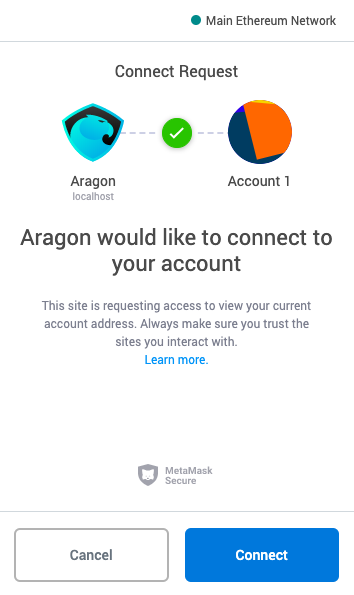
\includegraphics[width=0.4\textwidth]{Figures/metamask.png}
        \caption[Interfaz de metamask]{Interfaz de metamask cuando se pide permiso para conectar a una página. Wiki de Aragon. \cite{web:aragon}}
        \label{fg:aragon}
    \end{figure}
    Después de tener una conexión con su cartera \ref{fg:aragon}, necesitamos una vez mas su permiso. Como hemos comentado en el punto \textit{Introducción a la criptografía}, necesitamos la clave publica de la cartera. Es con esta clave con la que conseguiremos encriptar y desencriptar la información.
    \begin{lstlisting}
        const publicKey = await window.ethereum
			.request({
				method: 'eth_getEncryptionPublicKey',
				params: [account]
			});
    \end{lstlisting}
    De la siguiente forma, llamando al método \verb|eth_getEncryptionPublicKey| la podemos obtener. Nuevamente, para recordar, metamask vive \textit{fuera} de la \textit{burbuja de ejecución} de nuestro dominio. Esto significa que de manera literal necesitamos pedir permiso para realizar cualquier operación con la cartera del usuario.
    \item \textbf{Interactúa con una sala}\\
    \begin{itemize}
        \item \textbf{Crea la sala}\\
        Andes de crear esa sala, se necesitará generar las claves para definir la base de datos como una base de datos privada.
        \begin{lstlisting}
            const identity = await Identities.createIdentity(options);
        \end{lstlisting}
        Cuando ya tenemos nuestra identidad que va a ser usada para el transporte y para los permisos de escritura, podemos empezar a crear la sala.
        Esta sala es una base de datos que como se ha comentado anteriormente será \textbf{keyvalue}.
        \begin{lstlisting}
            const db = await orbitdb.keyvalue(account, options);
            await db.put(account, DID_safe);
        \end{lstlisting}
        Subimos nuestro DID para que el resto de personas puedan verlo al entrar y enviarnos información.
        Por ultimo, solo queda contactar con el smart contract con los métodos anteriormente vistos para poder avisar al resto de usuarios y actualizar la interfaz para avisar al usuario.
        \begin{lstlisting}
            contract.current.methods.createRoom(db.address.toString()).send({ from: account, gasPrice: '20000000000' });
        \end{lstlisting}
        A partir de este momento, otros usuarios pueden haber solicitado entrar en nuestra sala. Gracias a los métodos de escucha se traduce en unas notificaciones en la interfaz del usuario.
        Si decide aceptar alguna de esas notificaciones, se ejecutará las siguientes instrucciones.
        \begin{lstlisting}
            const jsonInterface = JSON.parse(identity);
        \end{lstlisting}
        Leemos la identidad que obtenemos del smart contract y lo parseamos con la clase JSON.
        \begin{lstlisting}
            await DB.current.access.grant('write', jsonInterface.id);
        \end{lstlisting}
        Finalmente podemos añadirle al grupo de personas capaces de escribir en la base de datos.
        \begin{lstlisting}
            contract.current.methods.acceptProposal(proposer).send({ from: account, gasPrice: '20000000000' });
        \end{lstlisting}
        Lógicamente, solo queda avisar al solicitante que puede conectarse.
        \item \textbf{Se una a una sala}\\
        Si el usuario quiere unirse a una sala existente, la secuencia de ejecución es diferente.
        Al igual que si queremos crear una sala, necesitamos generar las claves.
        \begin{lstlisting}
            const identity = await Identities.createIdentity(options);
        \end{lstlisting}
        Al no tener que iniciar la conexión por ahora, simplemente actualizamos la UI para avisar al usuario que toca esperar y solicitamos al smart contract la creación de una petición de entrada.
        \begin{lstlisting}
            contract.current.methods.createProposal(owner, JSON.stringify(identity)).send({ from: account, gasPrice: '20000000000' });
        \end{lstlisting}
        En algún momento, nuestra solicitud será aceptada y podremos conectarnos a la base de datos.
        \begin{lstlisting}
            const db = await orbitdb.open(url, {type: 'keyvalue'});
        \end{lstlisting}
        Abrimos la base de datos especificando la dirección obtenida desde el smart contract.
        \begin{lstlisting}
            // Replicate db in local storage
            await db.load();
        \end{lstlisting}
        Replicamos la base de datos, es decir, pedimos por PUBSUB a cualquier nodo si conoce la información y nos la puede proporcionar.
        \begin{lstlisting}
            await db.put(account, DID_safe);
        \end{lstlisting}
        Y finalmente, podemos subir nuestro nuestro DID para que nos puedan enviar fichero.
    \end{itemize}
    \item \textbf{Interactuamos con los peers}\\
    Como ya hemos compartido toda la información necesaria para hacer nuestro handshake distribuido, es hora de compartir información.
    Gracias a los eventos de replica de orbit db, podemos tener una cuenta de todos los usuarios y sus DID.
    Cuando un usuario quiere enviar un archivo a otro usuario, como se ha especificado en Estado del arte/Criptografía, tenemos que generar una clave común de encriptación/desencriptación y crear una \textit{caja} con esa clave de contenido.
    \begin{lstlisting}
        const syncKey = window.crypto.randomUUID();
        const encryptedSyncKey = encrypt(syncKey, peers[selectedAddress].publicKey);
    \end{lstlisting}
    Después de generar esa caja, solo queda encriptar el fichero y subirlo a IPFS.
    \begin{lstlisting}
        const file = await ipfs.current.add({ content: resultbytes });
        await DB.current.put(
			'to' + selectedAddress + '-' + window.crypto.randomUUID(),
			payload
		);
    \end{lstlisting}
    Para acabar, al ser una base de datos \textbf{keyvalue}, lo marcamos con \verb|tox823...-231324234124|. De esta forma podemos dividir la clave en dos por el guion y leer multiples ficheros sin necesidad de tener colisiones de nombres.
    El usuario que quiera descargar esa información, necesita desencriptar la \textit{caja}.
    \begin{lstlisting}
        const syncKey = await window.ethereum.request({
			method: 'eth_decrypt',
			params: [hexToDecrypt, account],
        });
    \end{lstlisting}
    Tenemos que solicitar permiso al usuario ya que vamos a usar su clave privada. Aunque no podemos verla porque \textbf{nunca} tenemos acceso a su clave privada.
    \begin{lstlisting}
        const stream = ipfs.current.cat(file.path);
    \end{lstlisting}
    Como ya tenemos la clave para abrir el fichero, podemos leer los contenidos y hacer el proceso contrario.
    \begin{lstlisting}
        const blob = new Blob([plaintextbytes], { type: 'application/download' });
        const blobUrl = URL.createObjectURL(blob);
        const FileSaver = require('file-saver');
        FileSaver.saveAs(blobUrl, fileName);
    \end{lstlisting}
    Por ultimo, importamos una librería ara poder descargar el fichero al usuario. 
    Estos pasos son repetibles todas las veces que se quieran y los ficheros están disponibles hasta que algún nodo de la red tenga ese fichero. También se puede \textit{pinnear} el fichero en un nodo remoto. Por ejemplo en los servidores de la universidad de Deusto.
\end{enumerate}
\newpage
\thispagestyle{empty}
\chapter{Planificación y presupuesto}\label{Planificación y presupuesto}
%Función que crea el título de capítulo y al cual se le da el nombre deseado a través de su parámetro obligatorio. Al no tener la función el “*” se escribirá también en el título del documento las palabras “Capítulo 1: …”. Además se indica, mediante la función “\label”, la correspondiente etiqueta que lleva asociada. La etiqueta sirve para que en caso de que luego se quiera hacer referencia al capítulo se haga llamando etiqueta tal que se escribiría “La información correspondiente a dicho tema se encuentra en el capítulo \ref{Int}.”

\thispagestyle{fancy}
%Función que determina que durante este capítulo se aplique el estilo Fancy.

\fancyhead[LE]{\thechapter.Planificación y presupuesto} 
%Función que se utiliza para indicar que en las páginas impares, aparezca en el encabezado en la parte izquierda, el número del capítulo con su correspondiente nombre.
El presupuesto de este proyecto se ha dividido en dos apartados claves: recursos humanos y recursos materiales.
\section{Recursos humanos}
Para poder tener un control de las horas dedicadas a este proyecto, se ha usado el tiempo dedicado más sobrecostes añadidos por semanas de trabajo extras. El proyecto originalmente estaba diseñado para dedicar 300 horas de trabajo a lo largo de un cuatrimestre de duración. El trabajo no se inició al inicio del cuatrimestre. Para empezar a computar las 300 horas de trabajo se necesitaba generar los objetivos y acotar todos los requisitos. Esta fase inicial ha tenido una duración de 100 horas; estas horas, se dedicaron a investigar el estado del arte alrededor del SSI y las tecnologías distribuidas. Para la creación de la memoria y la documentación del proyecto se utilizaron 100 horas más. Las 300 horas se dedicaron a analizar, diseñar, desarrollar y validar el proyecto. Desde, elegir las librerías y la blockchain a utilizar, hasta escribir todo el código necesario para generar una demo funcional. En total se computaron 500 horas de trabajo y utilizando un calculo de pago de 25\euro/hora, nos da un total de \textbf{12500\euro}.
\section{Recursos materiales}
Para el desarrollo de este proyecto, hay que contar con los materiales utilizados. Se ha usado un \textit{hardware} potente por su necesidad de procesamiento y RAM. En concreto hemos utilizado un portátil "Huawei matebook x pro 2017". El coste de este dispositivo es de \textbf{1000\euro}.
\section{Coste total}
\begin{table}[H]
    \centering
    \begin{tabular}{|l|c|}
        \hline
        \textbf{Recursos humanos}       & 12500\euro    \\
        \hline
        \textbf{Recursos materiales}    & 1000\euro     \\
        \hline
        \textbf{Total}                  & 13500\euro    \\
        \hline
    \end{tabular}
    \caption{Tabla con el desglose de costes del proyecto}
    \label{fg:dinero}
\end{table}
En esta tabla \ref{fg:dinero} se especifica todo el coste de planificación y desarrollo del proyecto.
\newpage
\thispagestyle{empty}
\chapter{Valoración ética}\label{Valoracion etica}
%Función que crea el título de capítulo y al cual se le da el nombre deseado a través de su parámetro obligatorio. Al no tener la función el “*” se escribirá también en el título del documento las palabras “Capítulo 1: …”. Además se indica, mediante la función “\label”, la correspondiente etiqueta que lleva asociada. La etiqueta sirve para que en caso de que luego se quiera hacer referencia al capítulo se haga llamando etiqueta tal que se escribiría “La información correspondiente a dicho tema se encuentra en el capítulo \ref{Int}.”

\thispagestyle{fancy}
%Función que determina que durante este capítulo se aplique el estilo Fancy.

\fancyhead[LE]{\thechapter.Valoración ética}
%Función que se utiliza para indicar que en las páginas impares, aparezca en el encabezado en la parte izquierda, el número del capítulo con su correspondiente nombre.

 Este proyecto busca responder a la necesidad de privacidad de la sociedad moderna. En la no tan reciente revolución del web 2.0 nuestros derechos digitales se han visto atacados ante grandes multinacionales. Cuando nos identificamos ante una página web dejamos restos de nuestra identidad. Esa información es extremadamente valiosa. Desde el escándalo de Cambridge Analytica la población busca una manera de protegerse de empresas que venden sus datos. Esta empresa, mientras estaba en funcionamiento, tuvo acceso a los datos de 85 millones de usuarios de Facebook. Estos usuarios no dieron consentimiento explícito para permitir el acceso a sus datos. Cambrice Analytica (CA, en adelante) solo tenía permiso de 270000 usuarios que usaron una aplicación llamada “This Is Your Digital Life”. Dando acceso a esa aplicación externa, CA tenía acceso a la información de esa persona y a toda la red de amigos de la misma. Una clara violación de no solo los términos de uso de Facebook sino de las leyes de privacidad europeas (GDPR-
RGPD) \cite{web:CA} . Este escándalo, entre otros muchos, es la motivación de este proyecto. En específico, nos encontramos con tres motivos éticos.
\begin{itemize}
    \item Cuidar la identidad y privacidad de las personas.
    \item Establecer un sistema para evitar el robo de identidad
    \item Crear un ecosistema para evitar la comercialización de los datos de las personas.
\end{itemize}
 Valorando los principios éticos antes mencionados, podemos desarrollar las siguientes normas de actuación.
\begin{itemize}
    \item Debe ser posible identificar a las personas sin requerir información personal.
    \item Cualquier flujo de datos debe estar permitido por el propietario de la información.
    \item Los datos y los usuarios deben estar protegidos.
    \item Los datos no deben salir del navegador del usuario o usuarios sin permiso de los mismos.
\end{itemize}
Para poder cumplir con las normas éticas establecidas, necesitamos un sistema de identificación mínimo. Esto significa que no identificamos a los usuarios por sus datos personales sino por la dirección de su cartera. Como por ejemplo:
\begin{quote}
    \verb|0x3aE9Ae282F922f3dA986f3F5e69e0EFbdE9BF348|
\end{quote}
Esto difiere con nuestro Documento Nacional de Identidad que usamos en nuestro dia a dia, ya que aunque los dos sirven para identificarnos, el DNI contiene información personal, la cual el propietario puede no querer su divulgación. Puede que una aplicación requiera saber la edad del usuario. Para poder llegar a ese conocimiento, se debe pedir permiso al usuario. Si el usuario no permite compartir esa información, no puede usar esa aplicación.\\
 Así mismo, gracias a este proceso podemos cumplir con la norma número 2. Todos las acciones que requieran de la información del usuario, deberán ser aprobadas.\\
 Para asegurar que los datos de nuestros usuarios están seguros, necesitaremos asegurar la inmutabilidad de la información. Esto se puede llegar a conseguir utilizando criptografía y blockchain. Gracias a las firmas criptográficas podemos asegurar matemáticamente que el emisor de la información es quien dice ser. No solo eso si no que podemos asegurar que dos ficheros son los mismos, sin necesariamente saber su contenido. Gracias a la criptografía y la blockchain, podemos asegurar a los usuarios que están comunicándose con quien cree que lo están haciendo y que sus archivos están seguros. Estos archivos solo se pueden desencriptar por quienes sean los destinatarios de los mismos. \\
 Por último, para poder garantizar la localización de los datos, utilizamos la descentralización. La descentralización, como ya ha sido explicado en el capítulo \ref{EdA} “Estado del arte”, significa que no existe un punto central  donde existen todos los datos. En cambio, cada uno tiene sus datos en un navegador y los puede compartir con quien desee. Esto nos garantiza que las comunicaciones son directas. No hay intermediarios en los que tener que confiar. Esto significa que nuestros datos no dejan un rastro del que preocuparse.\\
 Trás establecer la respuesta a las normas de actuación y desarrollar la solución, hay que analizar las hipotéticas consecuencias. El uso de la criptografía es un arma de doble filo, ya que cuanto más seguro se quiere el sistema, más poder computacional es necesario. La blockchain es un claro ejemplo de este problema. Ethereum, como analizado en el capítulo \ref{EdA} “Estado del arte”, utiliza \textit{proof-of-work} (PoW – Prueba de trabajo) para garantizar la seguridad de la cadena. Esto significa que para poder verificar una nueva transacción hay que gastar recursos computacionales. \\
 Con la creciente popularidad de las blockchain y en específico Ethereum, ha llevado a convertir \textit{proof-of-work} en una guerra armamentística. Cuanto más poder se tenga más transacciones se pueden verificar. En otras palabras, cuanto mayor es la inversión de los mineros mayor beneficio tienen. Si este proyecto consigue realizar sus objetivos, se necesitarán realizar más transacciones en la red, resultando en un mayor consumo energético que, en definitiva, concluye en contaminación asociada a la producción de energía.  Esto hace que el proyecto tenga una huella de carbono no ignorable. \\
 Finalmente, el conflicto ético resultante inclina la balanza a rechazar esta solución. Las consecuencias éticas de este proyecto superan a los beneficios. En términos tecnológicos y como ha sido explicado anteriormente en el capítulo \ref{EdA} “Estado del arte”, puede llegar a ser solucionado. En cambio, en términos éticos, la solución expuesta en este proyecto no es ética.
\newpage
\thispagestyle{empty}
\chapter{Conclusiones}\label{Conclusiones}
%Función que crea el título de capítulo y al cual se le da el nombre deseado a través de su parámetro obligatorio. Al no tener la función el “*” se escribirá también en el título del documento las palabras “Capítulo 1: …”. Además se indica, mediante la función “\label”, la correspondiente etiqueta que lleva asociada. La etiqueta sirve para que en caso de que luego se quiera hacer referencia al capítulo se haga llamando etiqueta tal que se escribiría “La información correspondiente a dicho tema se encuentra en el capítulo \ref{Int}.”

\thispagestyle{fancy}
%Función que determina que durante este capítulo se aplique el estilo Fancy.

\fancyhead[LE]{\thechapter.Conclusiones}
%Función que se utiliza para indicar que en las páginas impares, aparezca en el encabezado en la parte izquierda, el número del capítulo con su correspondiente nombre.
A lo largo de este proyecto se han presentado multitud de problemas relacionados con las identidades y los datos. Así mismo, también se han propuesto múltiples soluciones que pueden llegar a convertirse en el internet del mañana. Esta combinación de tecnologías no es nada más que un intento de predecir el futuro. Se dislumbra un futuro prometedor, pero por ahora solo es poco más que un concepto. Estas tecnologías no están preparadas para ser utilizadas en \textit{producción}. Tanto \verb|IPFS| como \verb|js-ipfs| están en \textit{alpha}. \verb|OrbitDB|, pilar central para coordinar la información, dice lo siguiente:
\begin{quote}
    NOTE! OrbitDB is alpha-stage software. It means OrbitDB hasn't been security audited and programming APIs and data formats can still change. We encourage you to reach out to the maintainers if you plan to use OrbitDB in mission critical systems. \cite{web:OrbitDBalpha}
\end{quote}
Es posible que el futuro no consiga ser totalmente descentralizado, pero por lo menos pueda llegar a ser lo más \textit{local-first} \cite{web:localfirst} posible. En definitiva un internet que tenga al usuario en centro, sin muros que dificulten la entrada y, sobre todo, sin cámaras.
\newpage
\thispagestyle{empty}
%Funciones para incluir los otros documentos que se han desarrollado. Dichos documentos son los distintos capítulos de la memoria. Toda la escritura de los mismos se realizará en los documentos de forma específica y no en este archivo “MAIN.tex”. Así que vamos a ellos.

\bibliographystyle{unsrt}
%Función que indica el estilo de bibliografía a utilizar.
\fancyhead[LE]{}
\bibliography{References.bib}
%Función que incluye la biblografía en el documento.
\newpage
\chapter{Glosario de abreviaturas}
\begin{table}[H]
    \centering
    \begin{tabular}{ c  c  c }
        DID     & Decentralized iDentifier          & Identificador descentralizado \\
        DNI     & -                                 & Documento Nacional de Identidad \\
        IPFS    & InterPlanetary File System        & Sistema de archivos interplanetario\\
        SSI     & Self-sovereign identity           & Identidad autosoberana \\
        DLT     & Distributed Ledger Technology     & Tecnología de Registro Distribuido \\
        P2P     & Peer-to-peer                      & Red entre iguales \\
        EBP     & European Blockchain Partnership   & Asociación Europea de Blockchain \\
        EBSI    & European Blockchain Services      & Infraestructura europea de servicios \\
                & Infrastructure                    & de cadena de bloques (blockchain) \\
        ESSIF   & European Self Sovereign Identity  & Marco Europeo de Identidad Auto \\
                & Framework                         & Soberana \\
        eIDAS   & electronic IDentification,        & Sistema Europeo de reconocimiento \\
                & Authentication and trust Services & de identidades electrónicas \\
        JSON    & JavaScript Object Notation        & Notación de objeto de JavaScript \\
        PoW     & Proof of Work                     & Sistema de prueba de trabajo \\
        PoS     & Proof of Stake                    & Sistema de prueba de participación \\
        SHA     & Secure Hash Algorithm             & Algoritmos de hash seguro \\
        DSL     & Domain-Specific language          & Lenguaje específico del Dominio \\
        EIP     & Ethereum Improvement Proposal     & Propuesta de Mejora de Ethereum \\
        CID     & Content IDentifier                & Identificador de contenido \\
        AES     & Advanced Encryption Standard      & Estándar de Encriptación Avanzada \\
        KPI     & Key Performance Indicator         & Indicador clave de rendimiento \\
        SSR     & Server-Side Rendering             & Representación del lado del servidor \\
        ISR     & Incremental Static Rendering      & Representación estática incremental \\
        HTML    & HyperText Markup Language         & Lenguaje de marcas de hipertexto \\
        API     & Application Programming Interface & Interfaz de programación de \\
                &                                   & aplicaciones \\
    \end{tabular}
\end{table}
\begin{table}[ht!]
    \centering
    \begin{tabular}{c c c}
        JS      & JavaScript                        & - \\
        CSS     & Cascading Style Sheets            & Hojas de estilo en cascada \\
        MVC     & Model-view-controller             & Modelo-vista-controlador   \\
        UI      & User Interface                    & Interfaz de usuario \\
        DB      & Database                          & Base de datos \\
        FTP     & File Transfer Protocol            & Protocolo de transferencia de \\
                &                                   & archivos \\
        CPU     & Central Processing Unit           & Unidad central de procesamiento \\
        RAM     & Random-Access Memory              & Memoria de acceso aleatorio \\
    \end{tabular}
\end{table}
\newpage
\chapter{Agradecimientos}
En primer lugar, me gustaría agradecer a la Universidad de Deusto y a mi entorno por hacer este viaje agradable y enriquecedor. A todos mis profesores, gracias \dots Pero sobre todo \dots \\
\\
A Diego López de Ipiña por confiar en mi e introducirme en la Web Distribuida.\\
\\
A Ama y Aita, por darme todo y regalarme todas las experiencias de mi vida.\\
\\
A mi tia por ayudarme con cualquier duda y estar siempre ahí para aconsejarme.\\
\\
A mis amigos por seguir ahí, aunque no les dediqué mucho tiempo.\\
\\
A todos, gracias \dots
\newpage
\chapter{Apéndice}
\section{README}
\begin{figure}[H]
    \centering
    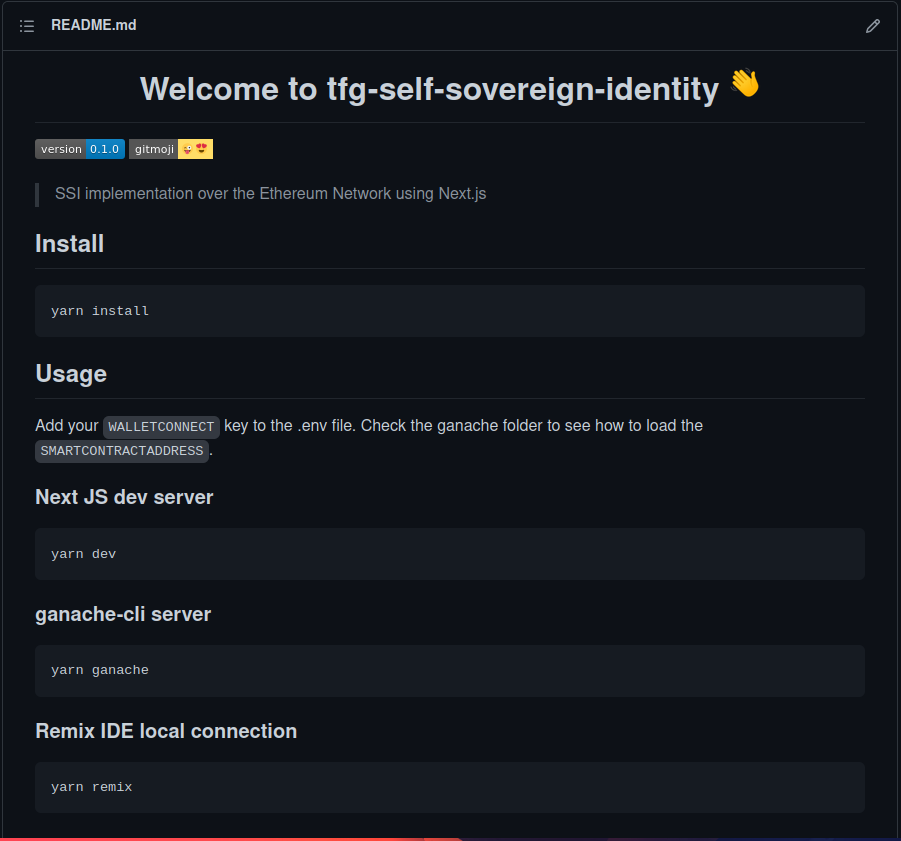
\includegraphics[width=1\textwidth]{Figures/gh1.png}
    \caption{README pt1}
    \cite{web:repo}
\end{figure}
\begin{figure}[H]
    \centering
    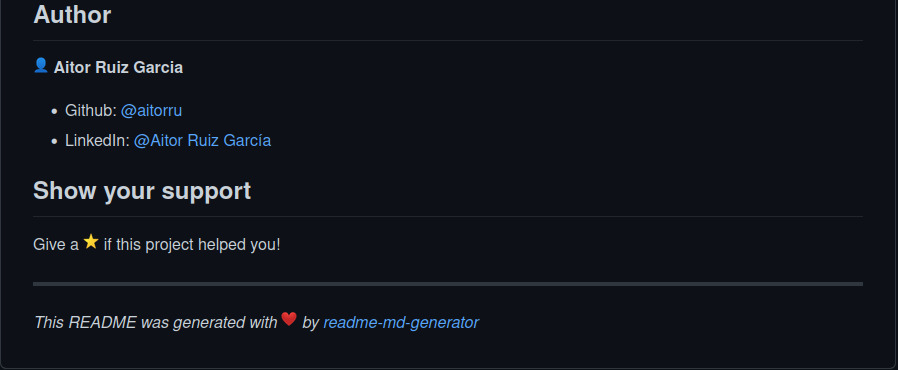
\includegraphics[width=1\textwidth]{Figures/gh2.png}
    \caption{README pt2}
    \cite{web:repo}
\end{figure}
\end{document}